\chapter{Experimentación} \label{ich:Experimentación}

En este capítulo explicaremos la experimentación realizada. Comenzaremos introduciendo las métricas empleadas para vigilar los procesos de entrenamiento de los distintos experimentos y evaluar la calidad de los modelos obtenidos, en la \sectionref{isec:metricas_teoria}. A continuación, en la \sectionref{isec:experimentos_realizados}, presentaremos los distintos experimentos realizados y expondremos los resultados obtenidos. Al principio lograremos unos resultados nefastos. Exploraremos otras bases de código para comprobar que estos resultados no se deban a un fallo por nuestra parte. Identificaremos la raíz del problema y propondremos una solución original a este. Validaremos la eficacia de nuestra solución a partir de una mejora sustancial de los resultados. Para acabar, en la \sectionref{isec:conclusiones_experimentacion} desarrollaremos las conclusiones obtenidas a partir de la experimentación.

\section{Métricas empleadas} \label{isec:metricas_teoria}

Como se comenta en el \entrecomillado{Apéndice D} de \cite{informatica:principal}, \textbf{el proceso de entrenamiento presenta una particularidad}: la función de pérdida rápidamente decae hasta un cierto valor en el que prácticamente se mantiene constante durante todo el entrenamiento. Sin embargo, otras métricas relevantes deberían mejorar durante el paso de las épocas de entrenamiento. Por tanto, \textbf{no es suficiente que observemos únicamente el valor de la función de pérdida}, sino que tenemos que seguir muy de cerca el valor de otras métricas relevantes durante el entrenamiento.

En esta sección introduciremos algunas de las métricas más relevantes. En toda esta sección, supondremos que estamos trabajando con $N$ individuos, cada individuo $i$ tendrá $N_i$ imágenes asociadas. Usaremos la misma notación que la introducida en \sectionref{isubs:seleccion_de_triples}. El elemento $x_k^p$ indicará que estamos trabajando con la imagen $k$ de la clase $p$. Solo que esta vez, estamos considerando todo el conjunto de datos.


\subsection{Distancias intracluster e intercluster} \label{isubs:teoria_distancia_intra_inter_cluster}

Como se comenta en \cite{informatica:paper_cacd}, el comportamiento esperado es el siguiente:

\begin{itemize}
    \item Al inicio, todos los elementos, independientemente de su identidad, serán atraídos hacia cierto centro de masa.
    \item Una vez hecho esto, elementos de distinta clase irán pasando a través de otros, formando los \textit{clústers} de cada individuo.
    \item Una vez que los \textit{clústers} establecen cierta estructura, estos empiezan a alejarse unos de otros.
\end{itemize}\

Todo esto ocurre mientras el valor de la función de pérdida parece no cambiar. Por tanto es relevante observar las siguientes dos métricas:

\begin{itemize}
    \item \textbf{Distancia intraclúster}: para cada individuo (o clase, en un ambiente más general), computamos la media de las distancias entre pares de imágenes de dicho individuo. Con esto, tenemos una lista de $N$ medias. Registraremos algunas estadísticas sobre esta lista de medias, como mínimo, máximo y media. Por tanto, la distancia intraclúster del individuo $p$ viene dada por:

    \begin{equation}
        D_{intra}^p := \frac{1}{N_p \cdot (N_p - 1)} \sum_{k = 1}^{N_p} \sum_{\substack{k' = 1 \\ k' \neq k}}^{N_p} D(x_k^p, x_{k'}^p)
    \end{equation}

    \item \textbf{Distancias interclúster}: para cada par de individuos distintos, computaremos la distancia mínima entre pares de puntos correspondientes a cada individuo. De estas distancias entre conjuntos volvemos a registrar las mismas estadísticas: mínimo, máximo y media. Por tanto, la distancia intraclúster entre los individuos $p$ y $p'$ viene dada por:

    \begin{equation}
        D_{inter}^{p, p'} := \min_{\substack{k \in \deltaset{N_p} \\ k' \in \deltaset{N_{p'}}}}{D(x_k^p, x_{k'}^{p'})}
    \end{equation}
\end{itemize}

Una vez definidas estas métricas, lo que esperamos ver durante el entrenamiento es que las distancias intraclúster se minimicen, mientras que las interclúster se maximicen.

\subsection{Normas de los \textit{embeddings}} \label{isubs:normas_embeddings}

Como ya hemos comentado en \sectionref{isec:triplet_loss}, un problema que puede ocurrir es que nuestro modelo decida colapsar cualquier entrada al vector $\vec{0}$. Esto justifica el uso de un margen. Pero en \sectionref{isec:margenes_suaves} hemos introducido una función para computar los márgenes de forma suave, sin especificar el valor del margen $\alpha$. Esta nueva variante podría dar lugar al colapso del modelo. Por tanto, vamos a observar durante el entrenamiento la norma euclídea de todas las salidas de nuestro modelo durante el entrenamiento. Esto es interesante sobre todo cuando no usamos la normalización de la salida, introducida en \sectionref{isubs:normalization_impl}.

\subsection{Sumandos activos}

En \sectionref{isubsubs:mejoras_sumandos_no_nulos} ya hemos desarrollado la noción de sumandos nulos y sumandos activos. Los sumandos nulos pueden llegar a ser nocivos para el aprendizaje de la red. Si demasiados triples no aportan valor a la función de pérdida, o bien no estamos aprovechando los ciclos de entrenamiento (en el caso de que estemos usando $\mathcal{L}_{BH \neq 0}, \mathcal{L}_{BA \neq 0}$) o bien  la red puede que no aprenda de los sumandos activos (en el caso de que estemos usando $\mathcal{L}_{BH}, \mathcal{L}_{BA}$). Por tanto, vamos a registrar el porcentaje de sumandos activos en la función de pérdida, en cada \textit{P-K batch} \footnotemark.

\footnotetext{Si el lector no está familiarizado con las funciones de pérdida $\mathcal{L}_{BH \neq 0}$, $\mathcal{L}_{BA \neq 0}$, $\mathcal{L}_{BH}$ o  $\mathcal{L}_{BA}$, estas son introducidas en \sectionref{isubs:seleccion_de_triples}. Por otro lado, el concepto de \textit{P-K batch} se introduce en \sectionref{isubs:muestreo_datos_pk_sampling_teoria}}

\subsection{\textit{Rank@k accuracy}} \label{isubs:rank_at_k}

A diferencia de un modelo de clasificación que trabaja con datos de la forma \lstinline{(imagen, etiqueta)}, no podemos calcular un valor de \textit{accuracy} directamente. Estamos tratando de resolver una tarea de \textit{retrieval}, por tanto, dada una imagen \textit{key} y una base de datos, buscamos las $k$  mejores imágenes dentro de la base de datos. Esto es, las $k$ imágenes que nuestro modelo identifica como las más similares a la identidad de la \textit{key} (gracias a nuestra función de distancia en el \textit{embedding}).

En esta situación podemos calcular es lo que se conoce como \textbf{\textit{Rank@k accuracy}}. Para ello, para cada imágen de nuestro \textit{dataset}:

\begin{itemize}
    \item Realizamos una \textit{query} a nuestro modelo, usando la imagen actual como \textit{key}, contra el resto de la base de datos, solicitando las $k$ mejores imágenes,.
    \item Calculamos si esta consulta ha tenido éxito. Consideramos por éxito que, entre las $k$ respuestas devueltas por la \textit{query}, al menos haya una que corresponda a la identidad de la \textit{key}.
\end{itemize}

Al final, sumamos los éxitos y dividimos por el tamaño de la base de datos, obteniendo el \textit{Rank@k accuracy}. Cabe destacar que no debemos confundir este valor de $k$, que indica cuántas imágenes consultamos en cada \textit{query}, con el valor de $K$ que usamos en el \textit{P-K sampling}. No tienen nada que ver un parámetro con el otro.

Hemos descrito el proceso usual de cómputo de esta métrica. Sin embargo, nosotros introducimos otra variante, a la que llamaremos \textbf{\textit{Local Rank@k accuracy}}. En esta variante, iteramos los datos en \textit{P-K batches}. Y con esto, las \textit{queries} las realizamos contra el \textit{P-K batch} y no contra toda la base de datos.


\section{Experimentos realizados} \label{isec:experimentos_realizados}

En esta sección introduciremos los distintos experimentos que hemos llevado a cabo, explicando el proceso realizado paso a paso. Comenzaremos con la \sectionref{isubsec:experimentacion_inicial} estudiando los experimentos iniciales sobre dos \textit{datasets} de caras distintos, en los que obtenemos resultados nefastos. Alcanzamos resultados de la misma calidad en \textit{MNIST} en la \sectionref{isubsec:experimentos_iniciales_mnist}. La simplicidad de este conjunto de datos nos hace pensar que o bien estamos aplicando erróneamente la técnica o bien que existe algún fallo en el diseño de esta. A continuación, en la \sectionref{isubsec:experiemntacion_base_codigo_externa}, exploramos distintos experimentos sobre \textit{MNIST} usando otras bases de código, para confirmar que un problema de diseño en la función de pérdida es la responsable de estos resultados y no un fallo por nuestra parte. Con todo lo aprendido, identificamos el motivo que causa el rendimiento nefasto y proponemos una solución original en la \sectionref{isubsec:identificacion_problemas_propuesta_solucion}. Para finalizar, en la \sectionref{isubsec:experimentacion_mnist_bien} y en la \sectionref{isubsec:experimentacion_cacd_bien} repetimos los experimentos aplicando nuestra propuesta, para \textit{MNIST} y \textit{CACD} respectivamente, mejorando los resultados enormemente, con lo que validamos la efectividad de la solución planteada.

Cabe destacar que el alcance inicial de este trabajo era el de aplicar las distintas técnicas que hemos ido desarrollando a los conjuntos de datos iniciales. Sin embargo, los resultados obtenidos son muy difíciles de defender, motivo por el cuál ha sido necesario encontrar la causa de estos, descartando un posible fallo por nuestra parte en la implementación y ejecución. Al haber encontrado esta causa, nuestro objetivo pasa a ser el de proponer una solución original y comprobar su eficacia. Por este cambio de objetivos y por falta de tiempo, no repetimos el \textit{hyperparameter tuning} para los nuevos experimentos.

\subsection{Experimentación inicial en \textit{CACD} y \textit{FG-Net}} \label{isubsec:experimentacion_inicial}

El alcance original del trabajo era el de aplicar distintas técnicas de minado de \textit{triplets online} para obtener un modelo que reconociera caras de forma invariante a la edad. Es por tanto, que a diferencia del resto de secciones, aplicamos todas las técnicas a nuestro alcance para mejorar el rendimiento del modelo, principalmente, \textit{hyperparameter tuning}.

\subsubsection{Selección de hiperparámetros} \label{isec:experimentacion_hp_tuning}

En la \sectionref{isec:hptuning_kfold_cross_validation} hemos descrito detalladamente el proceso para la selección de hiperparámetros y en la \sectionref{isec:hp_tuning} hemos descrito cómo implementamos este proceso. Describimos ahora cómo ejecutamos este proceso, las decisiones tomadas y qué información obtenemos.

Por el gran tamaño de los conjuntos de datos ha sido imposible ejecutar \textit{k-Fold Cross Validation} como método en el que basar la exploración de los hiperparámetros. Tanto por los enormes tiempos de cómputo como por el colapso de la memoria disponible en el \textit{hardware} empleado. Por tanto, nos vemos obligados a emplear \textit{holdout} como técnica base. Los problemas de robustez que esta técnica puede provocar se reducen al tener encuenta el gran tamaño de los conjuntos de datos con los que trabajamos. Al igual que hacen otros trabajos del estado del arte, realizaremos la exploración de hiperparámetros sobre \textit{CACD}. El conjunto de datos \textit{FG-Net} se usará únicamente para validar el modelo final.

La \tableref{table:rangos_hiperparametros} muestra los hiperparámetros que exploramos y el rango de valores que estos pueden tomar. Lanzamos la búsqueda de hiperparámetros para maximizar el valor de \textit{Rank@1 accuracy} \footnotemark. Los resultados de la búsqueda pueden consultarse en la base de datos \textit{SQLITE} \lstinline{hp_tuning_optuna.db} que está en nuestro repositorio de \textit{Github} \footnotemark. La \tableref{table:hp_escogidos} muestra los mejores hiperparámetros encontrados.

\footnotetext{Si el lector no está familiarizado con esta métrica, la hemos definido en \sectionref{isubs:rank_at_k}}
\footnotetext{Si el lector quiere realizar consultas sobre esta base de datos, el fichero \lstinline{optuna_queries.sql} contiene las órdenes \textit{SQL} que más hemos usado para vigilar el proceso de búsqueda.}

\begin{table}[!hbt]
\centering
    \begin{tabular}{|l|p{5cm}|}
    \hline
    \textbf{Hiperparámetros} & \textbf{Rango de valores} \\
    \hline

    P & $[2, 10]$ \\
    K & $[2, 10]$ \\
    Arquitectura de la red & \textit{CACDResNet18}, \textit{CACDResNet50} \textit{FGLightModel} \\
    Función de pérdida & \textit{Batch All}, \textit{Batch Hard} \\
    Uso de normalización & Sí, No \\
    Dimensión del \textit{embedding} & $\deltaset{10}$ \\
    \textit{Learning Rate} & $[0, 0.001]$ \\
    Uso de \textit{Softplus} & Sí, No \\
    Penalización en la norma de las salidas & Sí, No \\
    Factor de penalización en la norma de las salidas (*) & $[0.0001, 2.0]$ \\
    Uso de \textit{Gradient Clipping} & Sí, No \\
    Valor máximo del \textit{Gradient Clipping} (*) & $[0.00001, 10.0]$ \\
    $\alpha$ (*) & $[0.001, 1.0]$ \\

    \hline

\end{tabular}
\caption{Hiperparámetros a explorar y el rango de valores que pueden tomar. Los hiperparámetro marcados con (*) dependen del valor de otros hiperparámetros. En el caso de usar \textit{Softplus} no debemos establecer el valor del margen. Los valores de penalización y \textit{gradient clipping} solo se usan si decidimos usar estas técnicas, respectivamente.}
\label{table:rangos_hiperparametros}
\end{table}

\begin{table}[!hbt]
\centering
\begin{tabular}{|l|l|}
    \hline
    \textbf{Hiperparámetro}                           & \textbf{Valor escogido} \\
    \hline
    P                                                 & 8                       \\
    K                                                 & 2                       \\
    Arquitectura de la red                            & \textit{CACDResNet18}   \\
    Función de pérdida                                & \textit{Batch Hard}     \\
    Uso de normalización                              & No                      \\
    Dimensión del \textit{embedding}                  & 9                       \\
    \textit{Learning Rate}                            & $5,157 \cdot 10^{-4}$   \\
    Uso de \textit{Softplus}                          & No                      \\
    Penalización en la norma de las salidas           & No                      \\
    Factor de penalización en la norma de las salidas & -                       \\
    Uso de \textit{Gradient Clipping}                 & No                      \\
    Valor máximo del \textit{Gradient Clipping}       & -                       \\
    $\alpha$                                          & 0.840                   \\

    \hline
\end{tabular}
\caption{Valores de los hiperparámetros escogidos a partir del proceso de \textit{hyperparameter tuning}. Con estos parámetros obtenemos un valor máximo de \textbf{\textit{Rank@1} de 0.0945}. Los hiperparámetros con un valor \entrecomillado{-} son valores de técnicas que hemos elegido no usar. Resultados obtenidos sobre el conjunto de datos \textit{CACD}.}
\label{table:hp_escogidos}
\end{table}

En la \tableref{table:hp_escogidos} podemos ver que el valor máximo alcanzado para \textit{Rank@1 Accuracy} es realmente malo, no llega al $0.1$. Por otro lado, de 92 pruebas de hiperparámetros, solo 11 consiguen terminar su ejecución de forma normal. Es decir, el 88\% de las pruebas fallan, la mayoría por explosión de gradientes. Esto ya indica dos inconvenientes de las nuevas técnicas que estudiamos en este trabajo:

\begin{enumerate}
    \item Producen modelos con un rendimiento muy bajo, que no pueden usarse en la práctica y que están muy lejos de haber aprendido a solventar la tarea en cierta medida, mucho menos de ser comparables a los modelos estados del arte.
    \item Provocan que el entrenamiento del modelo sea muy frágil y que sea realmente complicado encontrar configuraciones de hiperparámetros que produzcan un modelo sin errores en el proceso.
\end{enumerate}

En base a estos resultados, entrenaremos un modelo sobre todo el conjunto \textit{CACD} y validaremos los resultados sobre \textit{FG-Net}. Para ello, usaremos los hiperparámetros que hemos encontrado en la \tableref{table:hp_escogidos}. Esperamos obtener muy malos resultados, pues ya hemos comentado que \textit{FG-Net} es un conjunto de datos más complicado que \textit{CACD}, y el valor tan bajo de \textit{Rank@1 Accuracy} no es nada esperanzador.

\subsubsection{Descripción del modelo empleado} \label{isec:explicacion_modelo}

Como hemos visto en la \tableref{table:hp_escogidos}, hemos decidido usar el modelo \textit{CACDResnet18}, que es una adaptación del modelo \textit{ResNet18} que tiene dos objetivos. El primero de ellos, trabajar con el conjunto de datos \textit{CACD} en vez de con el conjunto de datos \textit{ImageNet}. El segundo de ellos, producir un \textit{embedding}, de dimensión 9 en base a la \tableref{table:hp_escogidos}, en vez de resolver una tarea de clasificación con 1000 clases de salida. Para realizar esta adaptación, simplemente cambiamos la última capa de \textit{ResNet18} que pasa de ser una capa densa con 1000 valores de salida a ser una capa densa con 9 valores de salida. Además, usamos la red pre-entrenada del paquete \lstinline{torchvision} \cite{informatica:resnet18_torchvision}. Realizamos un ajuste fino de todas las capas de la red, es decir, no congelamos ninguno de los parámetros del modelo.

La arquitectura original fue introducida en \cite{informatica:resnet_original_paper}. La idea principal consiste en trabajar con bloques residuales y \textit{skip connections} con el objetivo de que el gradiente fluya mejor y así poder emplear un gran número de capas, es decir, aumentar drásticamente la profundidad. De ahí su nombre, \textit{RESiudal NETwork}. A continuación describimos estas dos componentes principales del modelo:

\begin{itemize}
    \item Un \textbf{bloque residual} se compone de dos capas convolucionales. Entre las dos capas convolucionales aplicamos una no-linealidad (\textit{ReLU}, en la arquitectura original). Además sumamos la entrada original a la salida. Tras esto, se aplica otra no-linealidad. Es decir, dado una entrada $X$, computamos $\mathcal{F}(X) + X$. Por tanto, la red no aprende drectamente la salida buscada, sino la diferencia entre la entrada y dicha salida. Todo esto queda reflejado en la \imgref{img:ejemplo_bloque_resnet}.
    \item Las \textbf{\textit{skip connections}} pasan la información directamente de una capa a otra, saltándose uno o más bloques residuales. Esto permite que no haya tanto desvanecimiento del gradiente, lo que permite usar más bloques residuales (aumentando drásticamente la profundidad).
\end{itemize}

\begin{figure}[hbt]
    \centering
    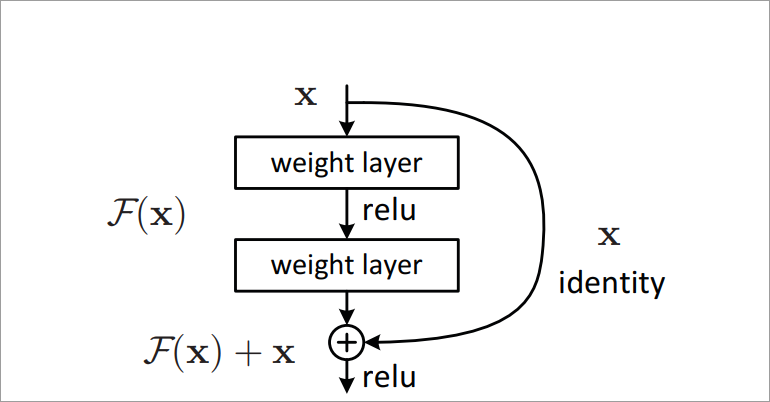
\includegraphics[width=0.6\textwidth]{informatica/bloque_resnet}
    \caption{Ejemplo de bloque residual. Imagen extraída de \cite{informatica:resnet_original_paper}}
    \label{img:ejemplo_bloque_resnet}
\end{figure}

En base a estos elementos, la arquitectura de nuestro modelo \textit{ResNet18} se describe gráficamente en la \imgref{img:arquitectura_resnet_18}. Notar que estamos modificando la última capa \textit{fully connected}, pasando de 1000 valores de salida a solo 9 (la dimensión de nuestro \textit{embedding}).

\begin{figure}[!hbt]
    \centering
    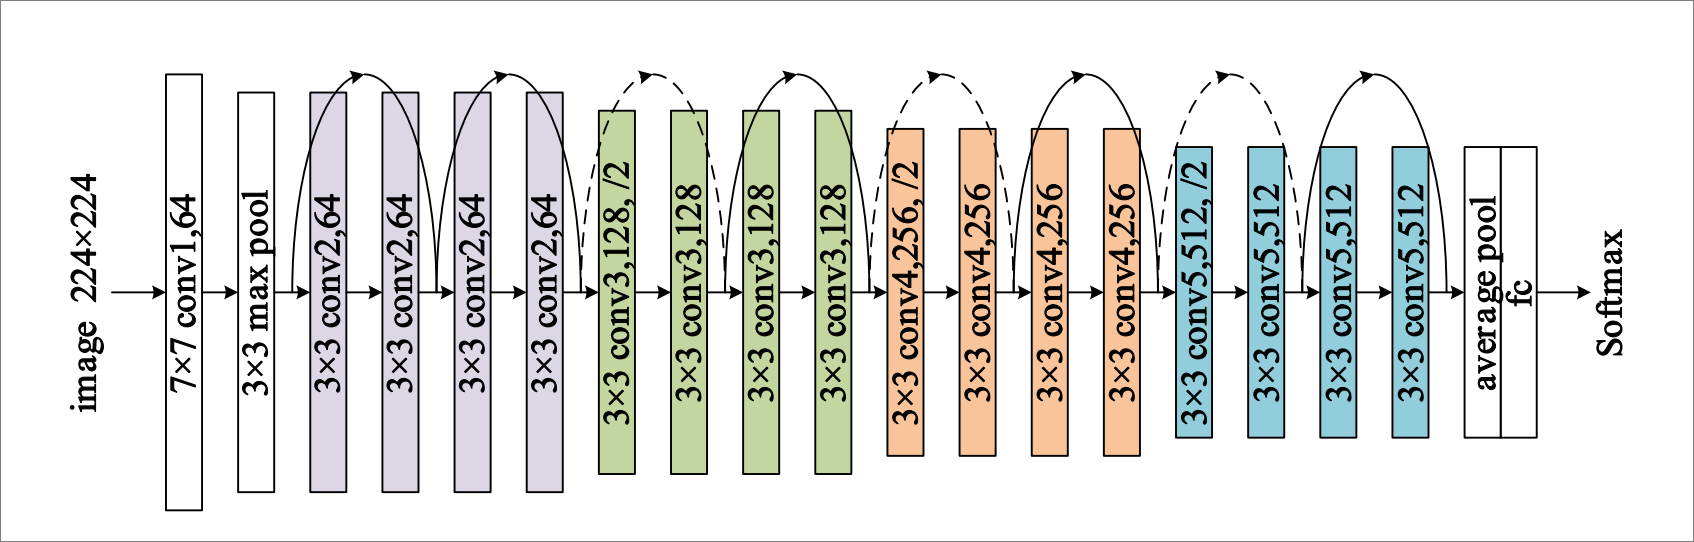
\includegraphics[width=1.0\textwidth]{informatica/resnet18_arch}
    \caption{Diagrama de la arquitectura \textit{ResNet18}. Las líneas continuas por encima de los bloques indican la conexión entre el inicio y final de un bloque residual. Las líneas discontinuas por encima de los bloques indican las \textit{skip connections}. Imagen extraída de \cite{informatica:resnet18_arch_web}}
    \label{img:arquitectura_resnet_18}
\end{figure}

\subsubsection{Entrenamiento del modelo y resultados obtenidos} \label{isec:entrenamiento_mejor_modelo}

Entrenamos el modelo usando los hiperparámetros indicados en \tableref{table:hp_escogidos}. Además, especificamos los siguientes hiperparámetros:

\begin{itemize}
    \item Modificación de la función de pérdida para usar únicamente los sumandos activos, es decir, $\mathcal{L}_{BH \neq 0}$.
    \item Épocas de entrenamiento: una única época de entrenamiento. El conjunto de entrenamiento \textit{CACD} es lo suficientemente grande como para entrenar en una sola época. Tomamos esta decisión en base a experimentos previos y a los propios resultados de este entrenamiento..
    \item Técnica de Aumentado de Datos: \textit{lazy}. Esta variante permite que no saturemos la memoria disponible. De otra forma, en algunos experimentos obtenemos errores al ocurrir dicha saturación de la memoria.
    \item Usamos el 80\% del \textit{dataset} \textit{CACD} para entrenar, y el 20\% restante como conjunto de validación.
\end{itemize}

El proceso de entrenamiento puede estudiarse a partir de las métricas que se muestran en \imgref{img:metricas_entrenamiento}. Al finalizar el entrenamiento, evaluamos distintas métricas sobre el conjunto \textit{FG-Net}. Estos resultados se muestran en la \tableref{table:resultados_sobre_fg_net}.


\begin{figure}[!hbtp]

    \centering
    \begin{subfigure}[t]{0.45\textwidth}
        \includegraphics[width=1.0\textwidth]{informatica/wandb/entrenamiento_principal/running_loss}
        \caption{Error de entrenamiento tipo \entrecomillado{running}}
    \end{subfigure}
    \begin{subfigure}[t]{0.45\textwidth}
        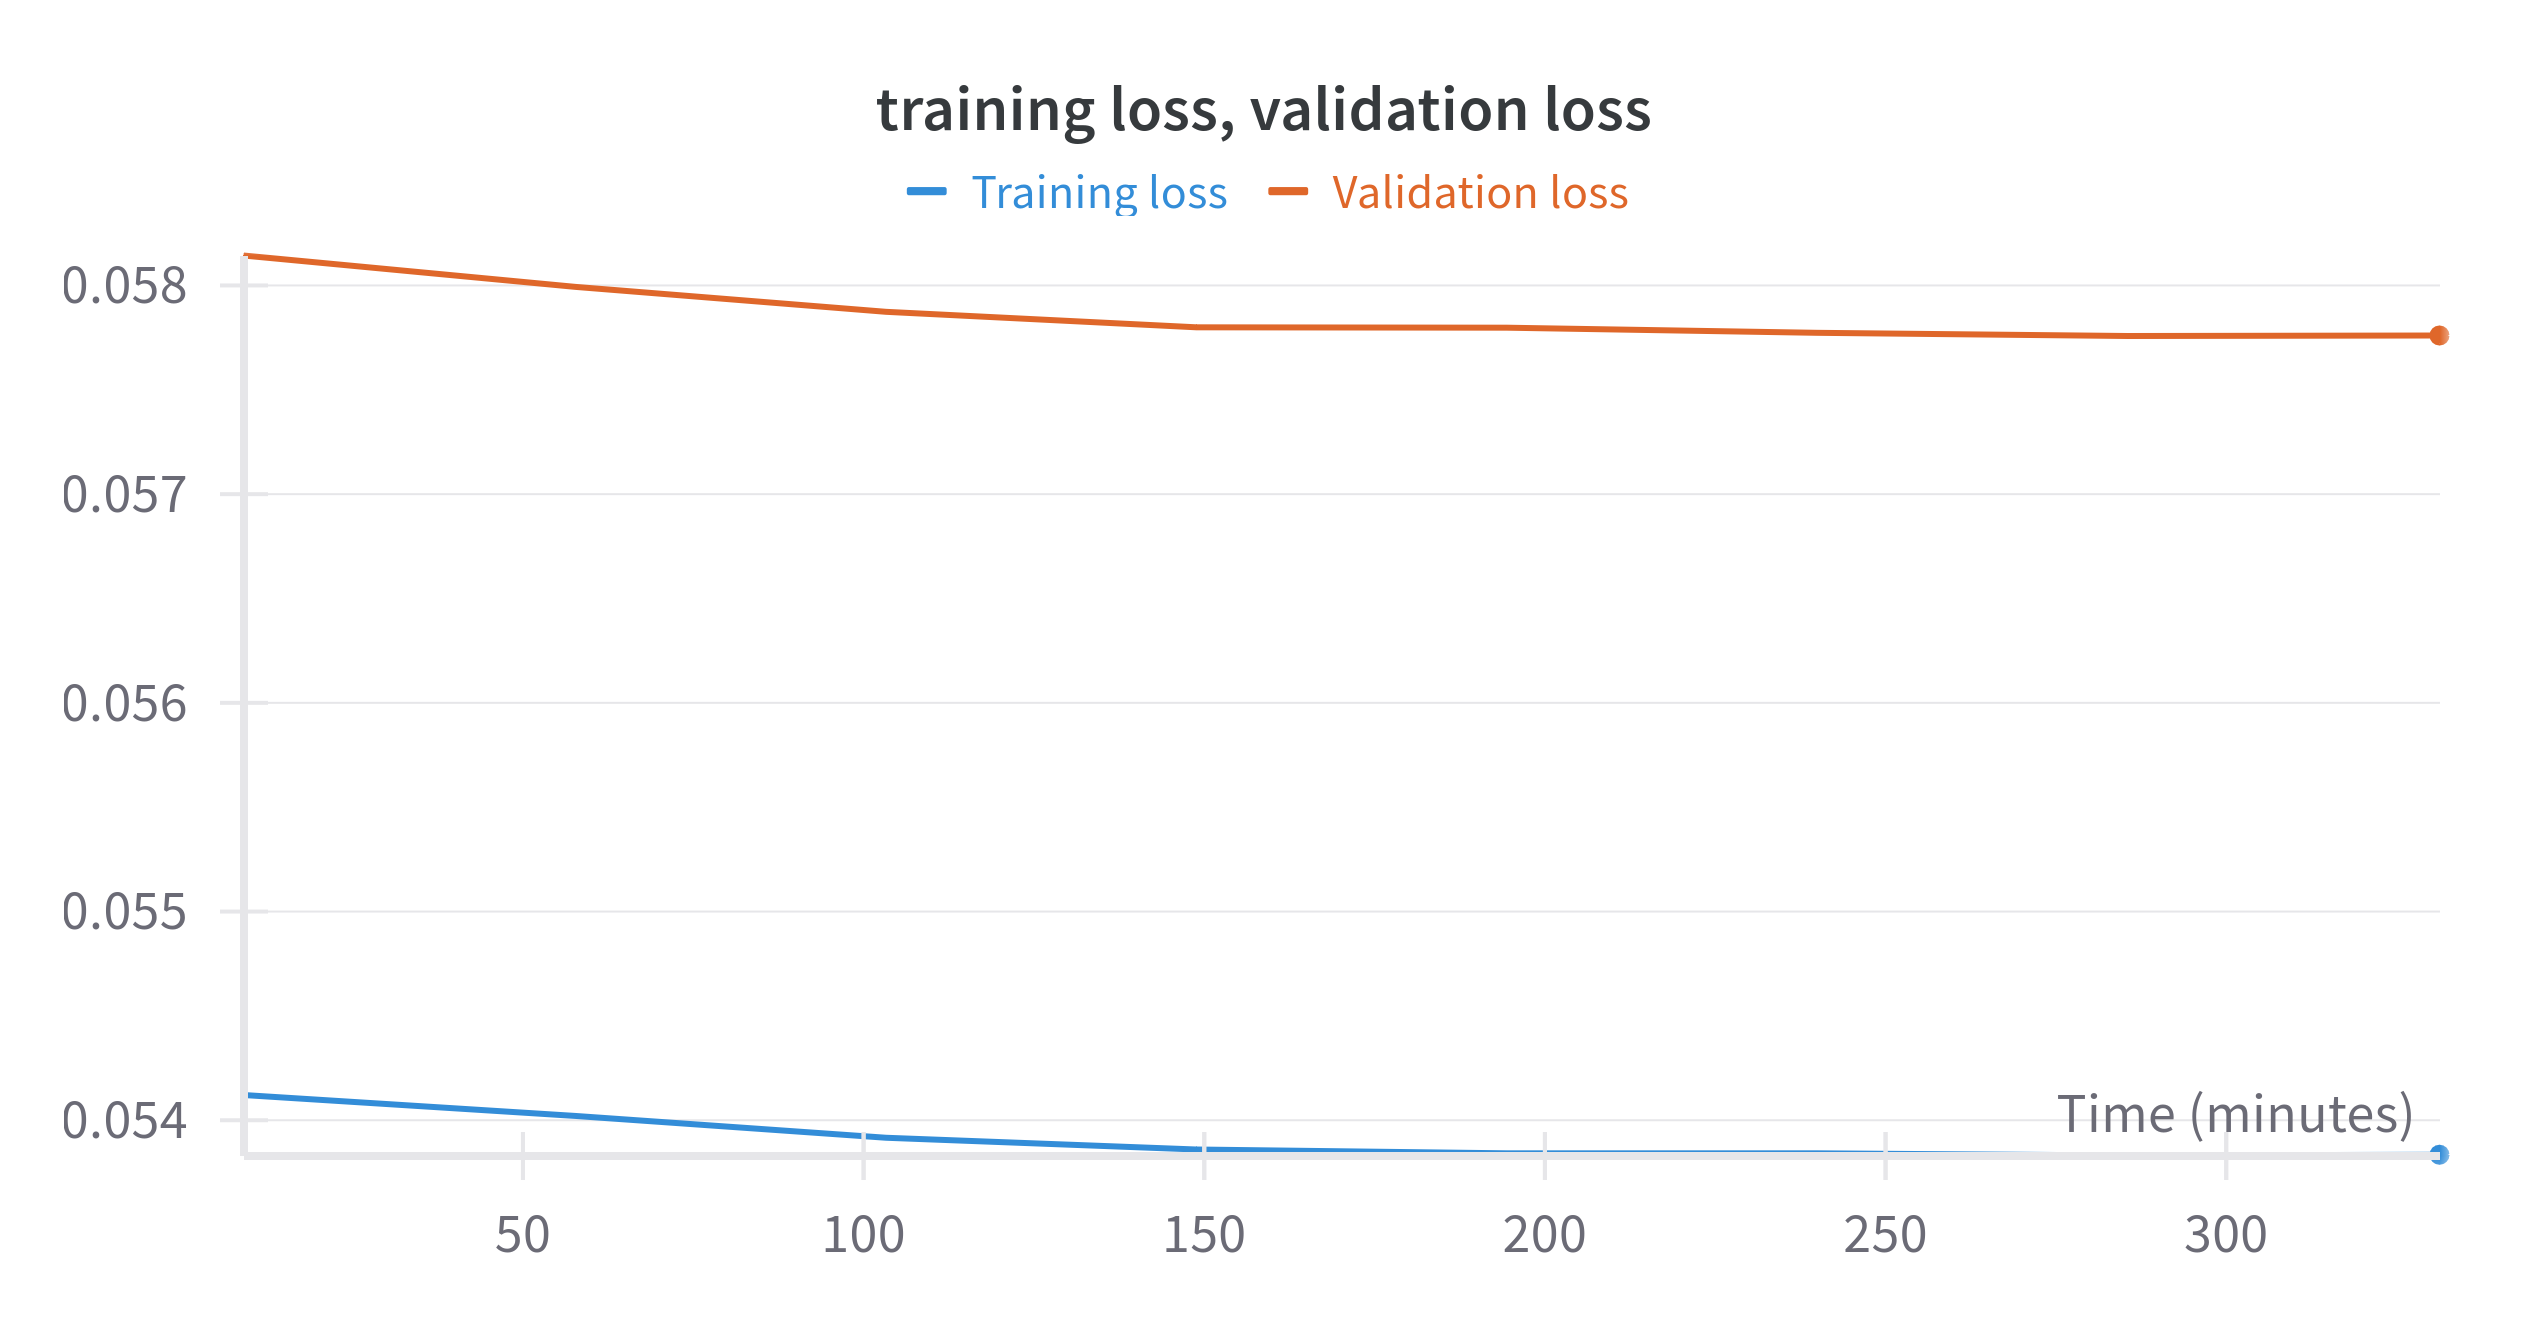
\includegraphics[width=1.0\textwidth]{informatica/wandb/entrenamiento_principal/manual_loss}
        \caption{Error de entrenamiento}
    \end{subfigure}

    \begin{subfigure}[t]{0.45\textwidth}
        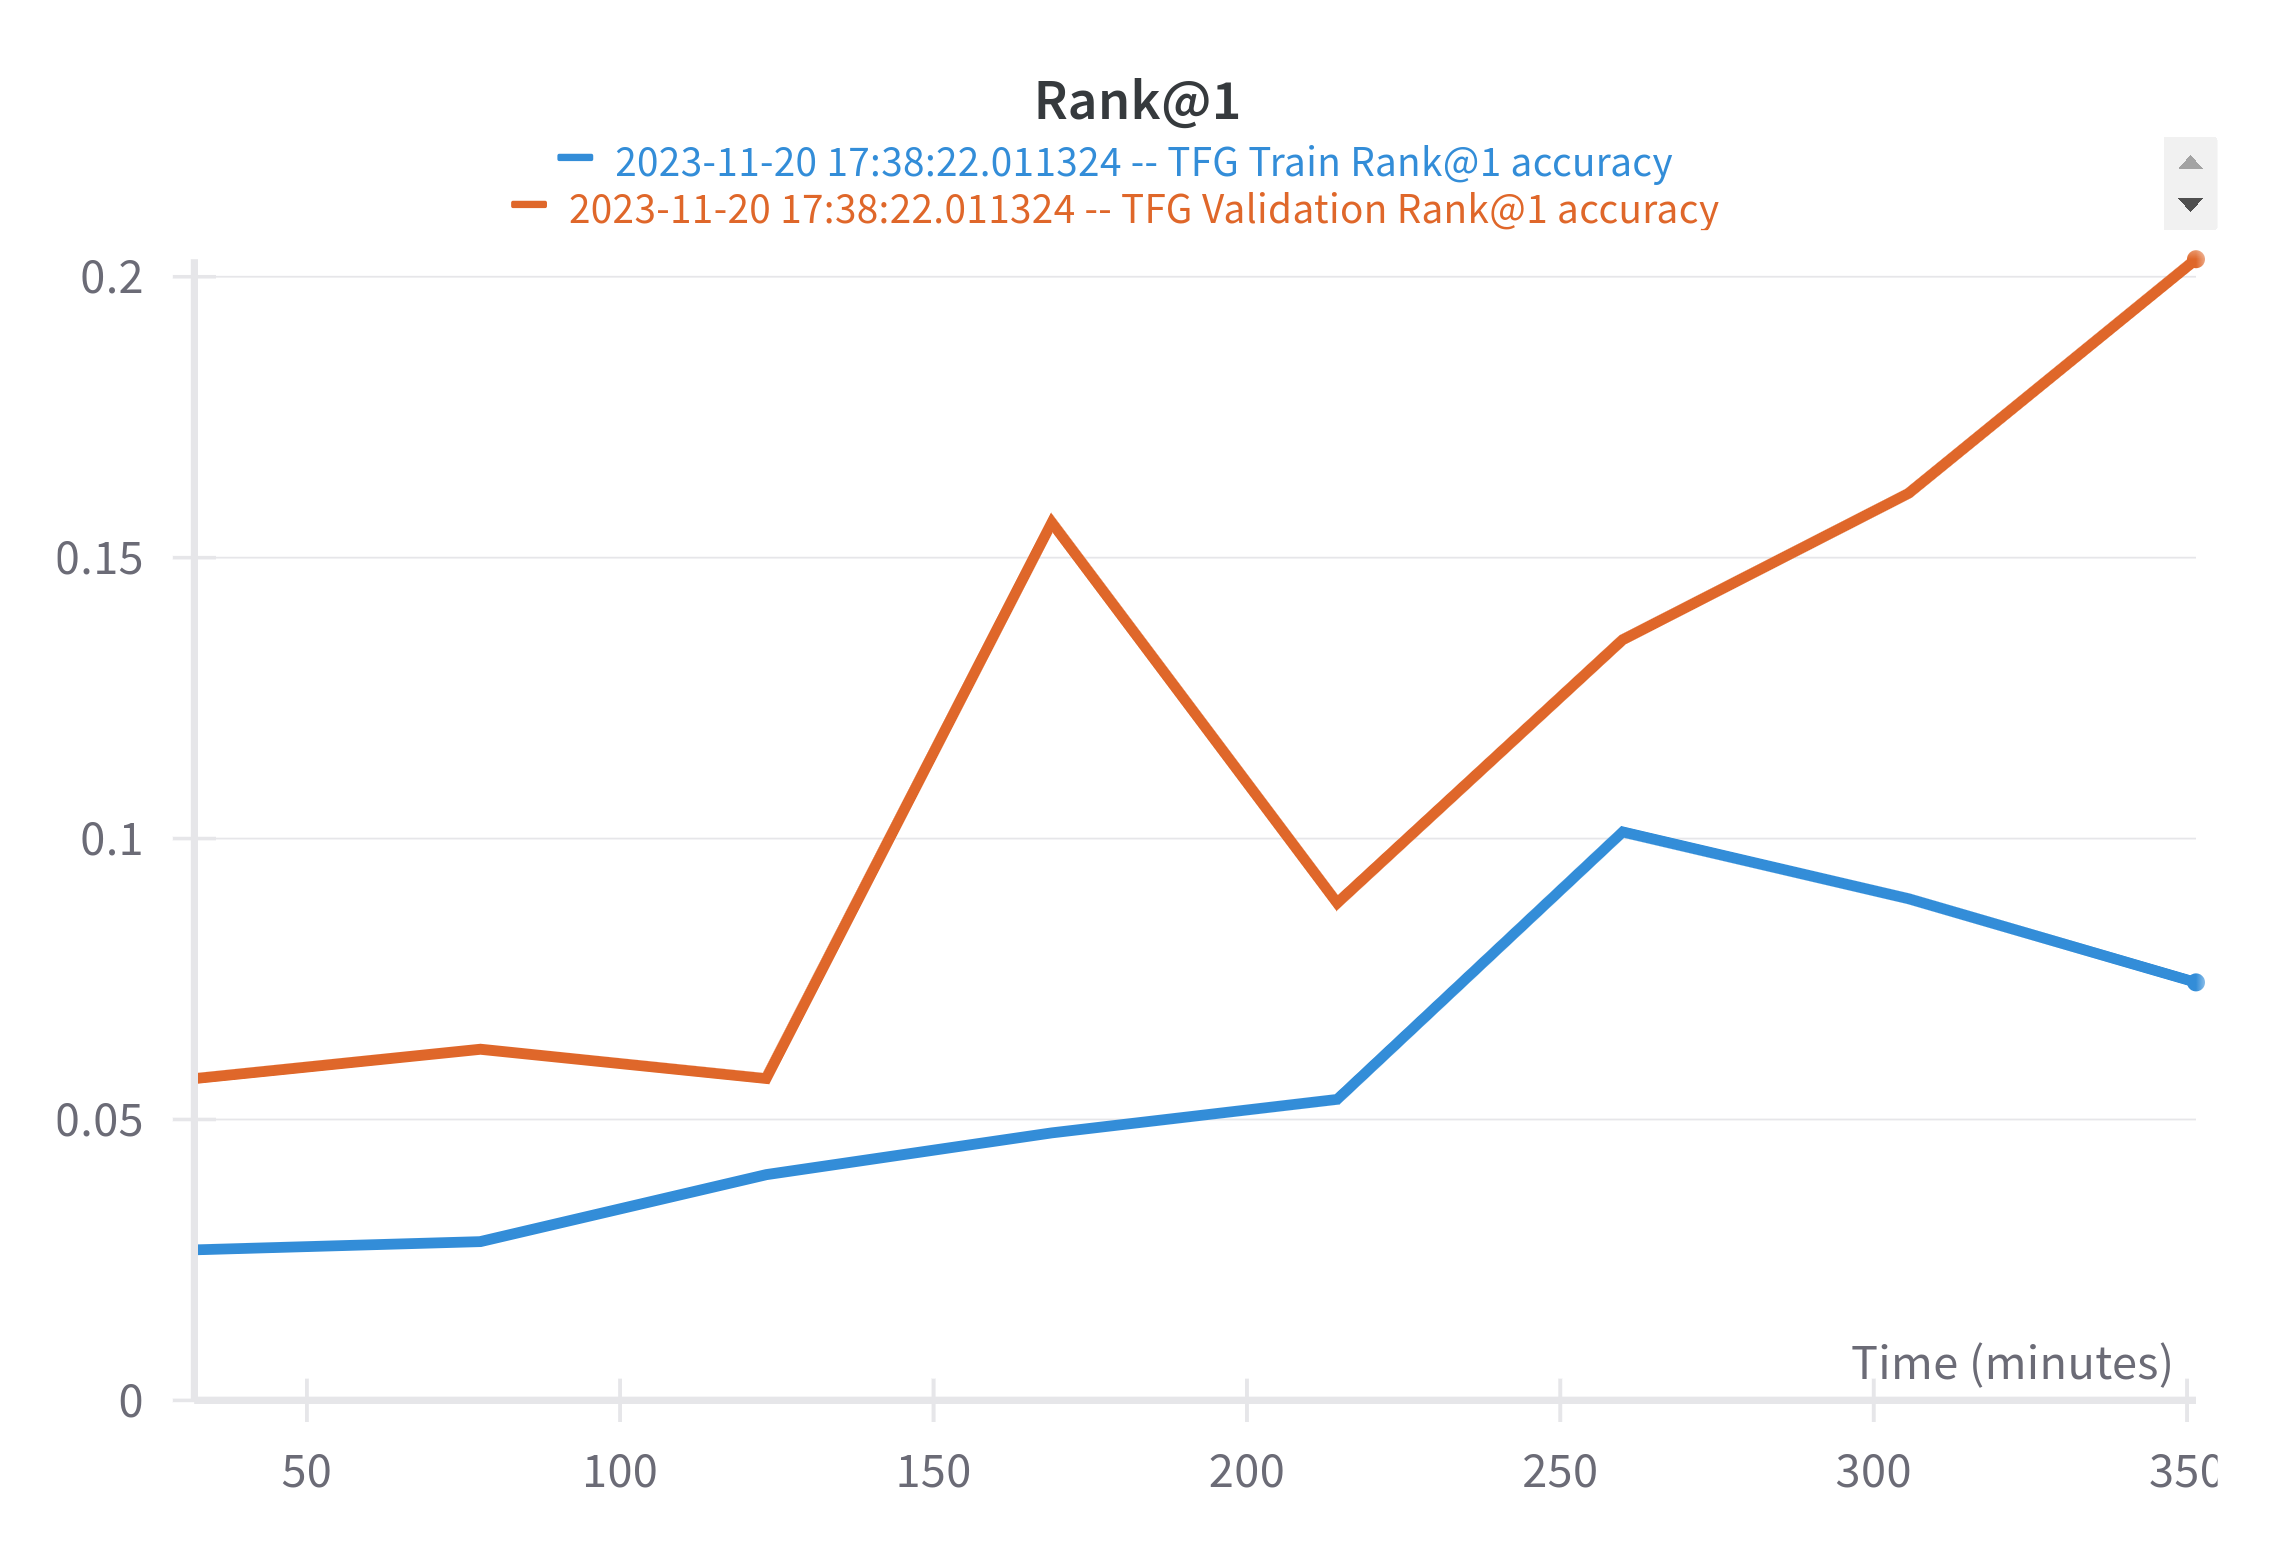
\includegraphics[width=1.0\textwidth]{informatica/wandb/entrenamiento_principal/rank@1}
        \caption{\textit{Rank@1 Accuracy}}
    \end{subfigure}
    \begin{subfigure}[t]{0.45\textwidth}
        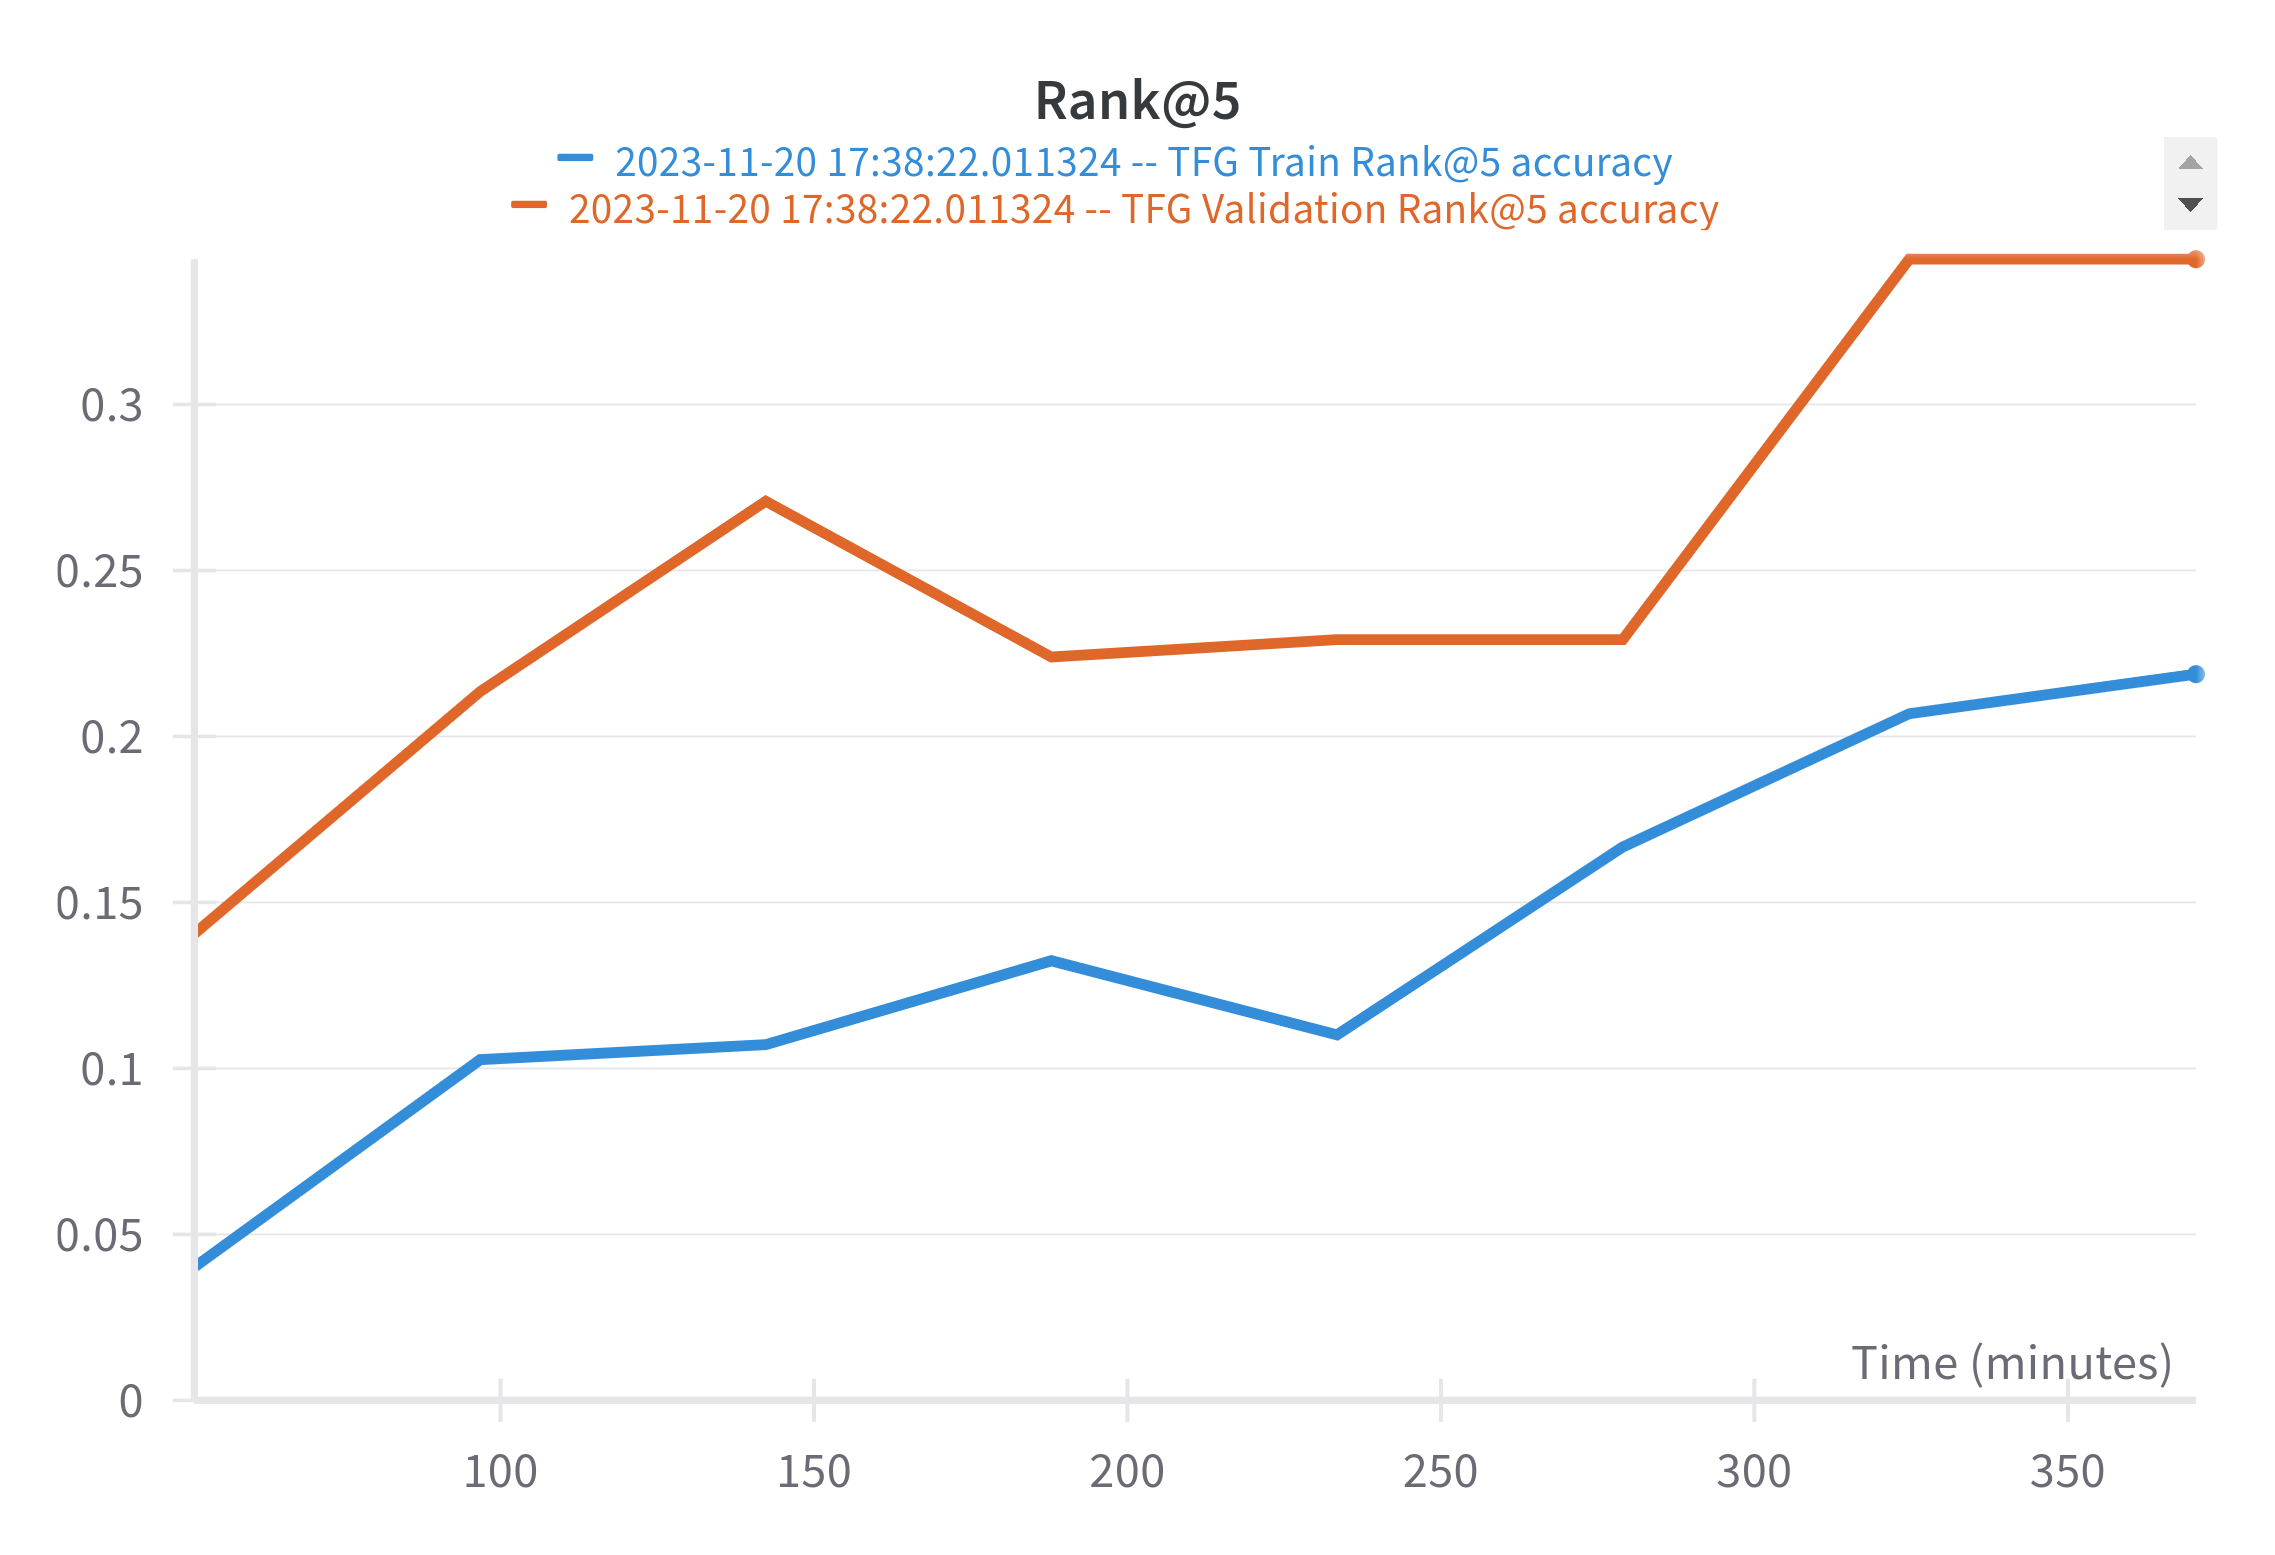
\includegraphics[width=1.0\textwidth]{informatica/wandb/entrenamiento_principal/rank@5}
        \caption{\textit{Rank@5 Accuracy}}
    \end{subfigure}

    \begin{subfigure}[t]{0.45\textwidth}
        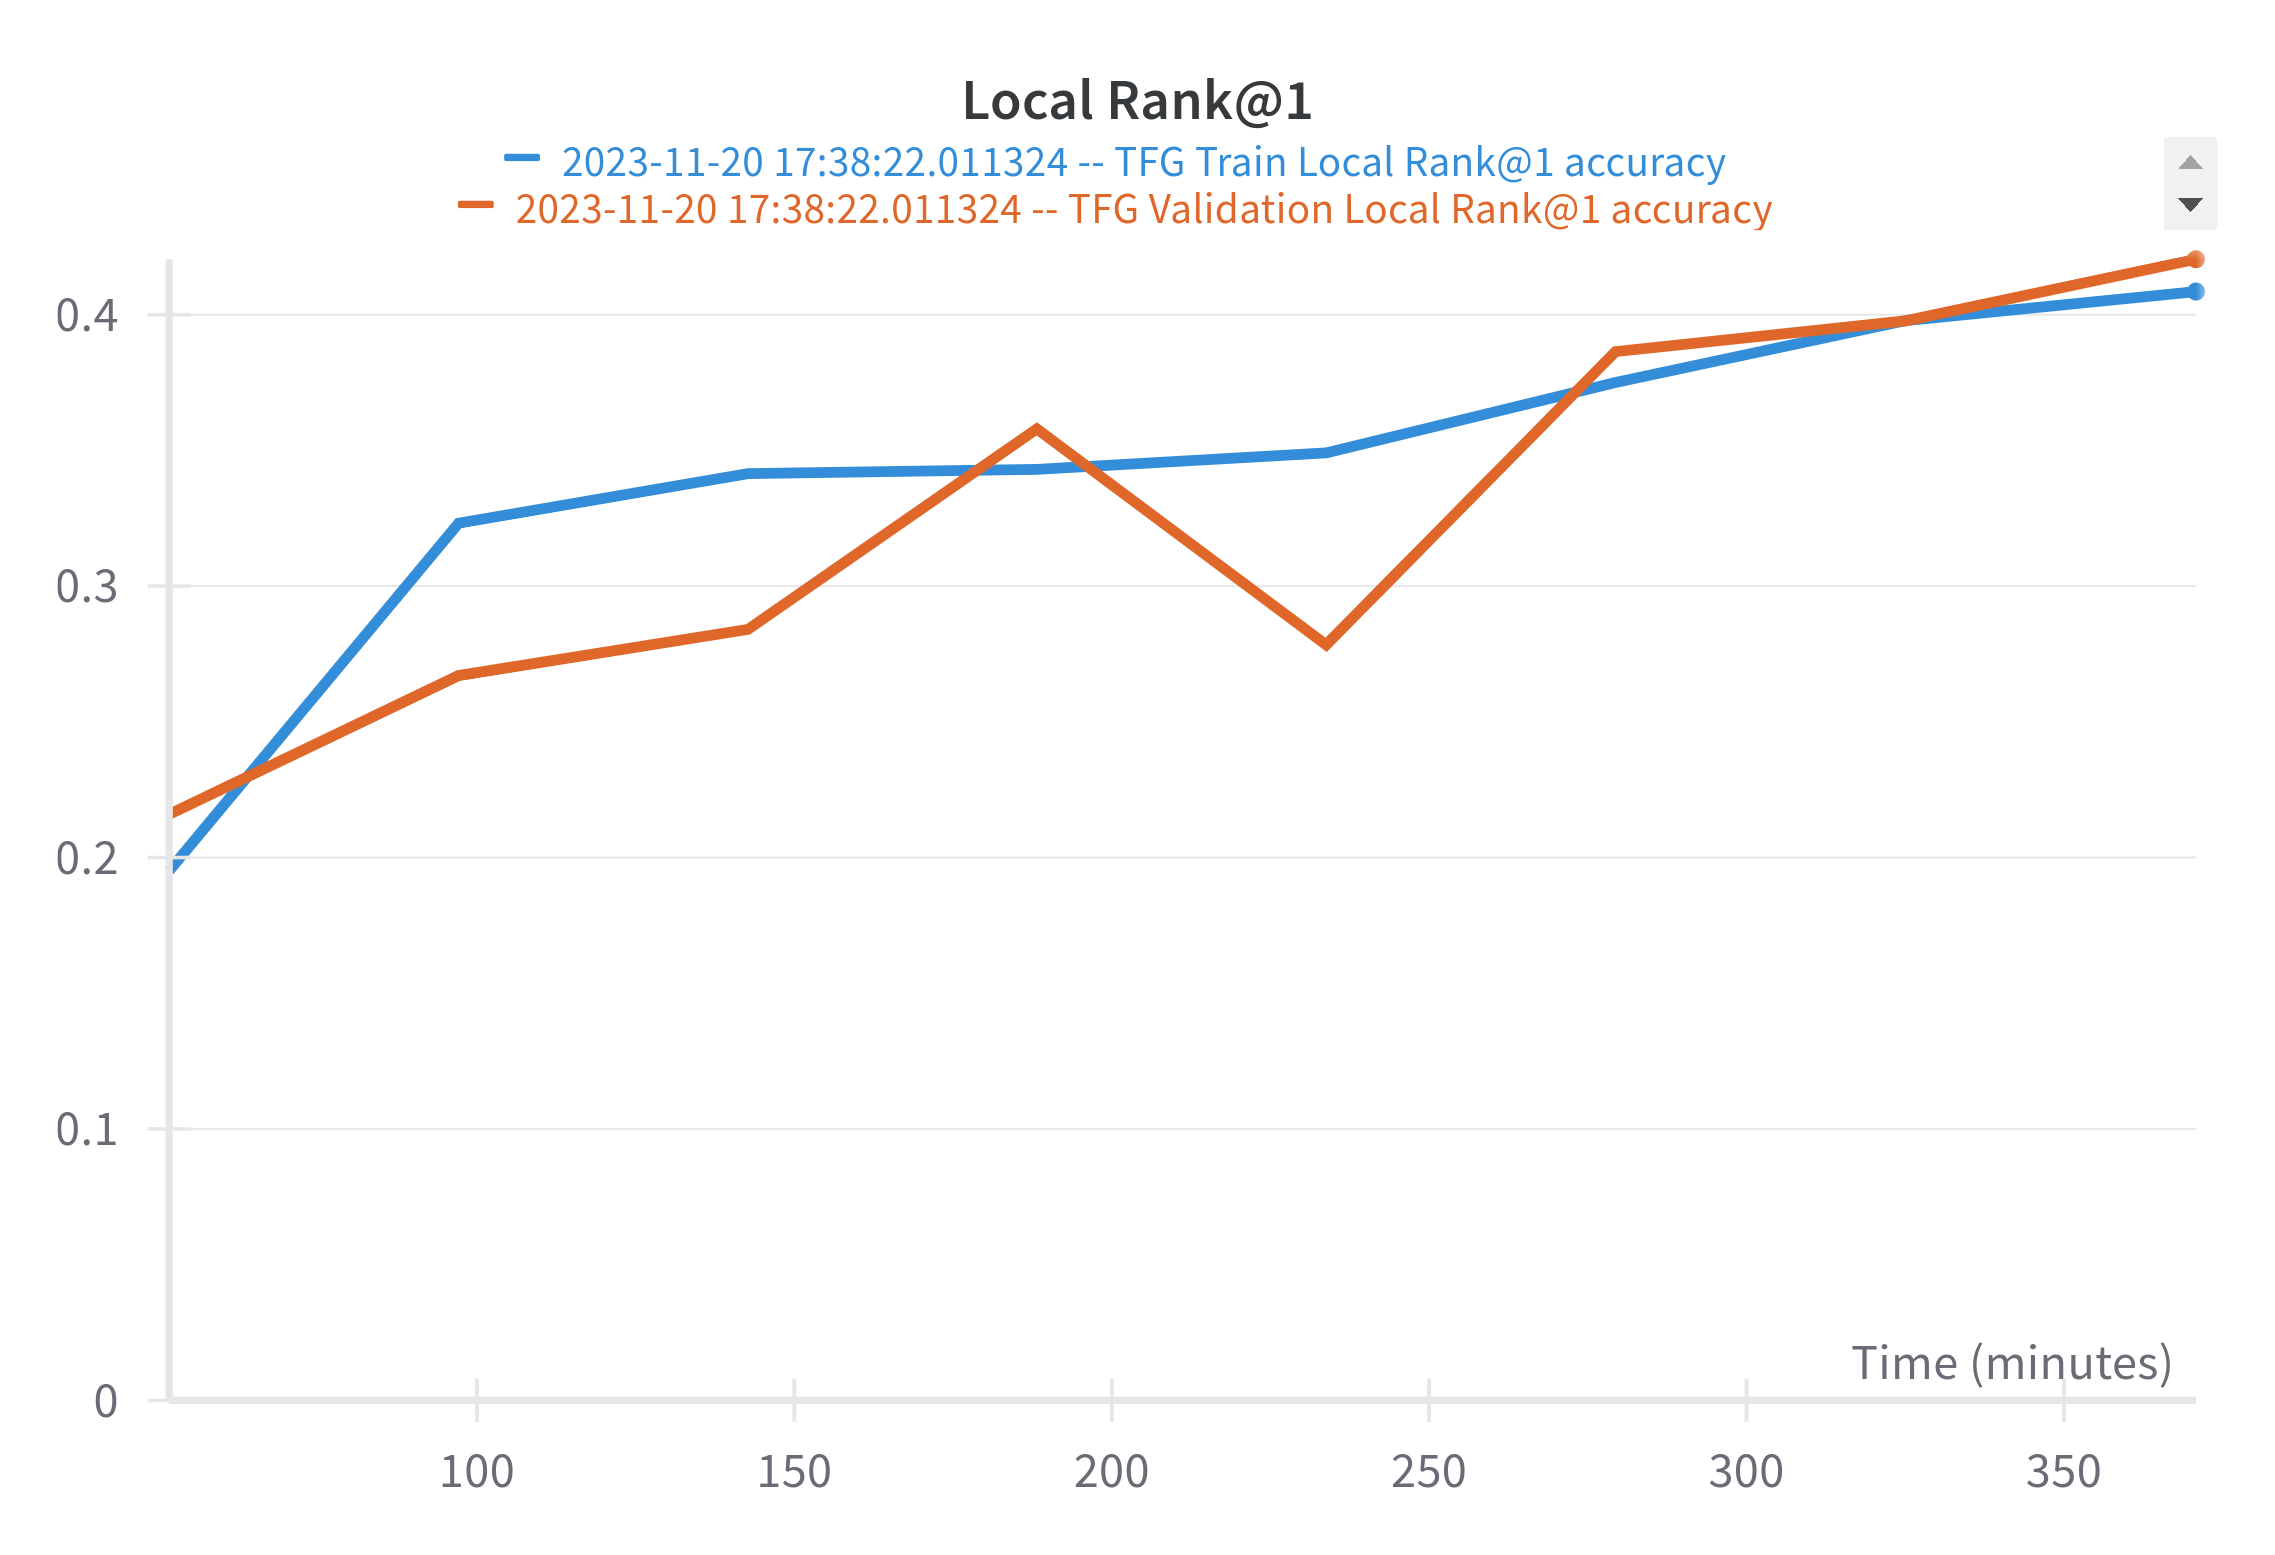
\includegraphics[width=1.0\textwidth]{informatica/wandb/entrenamiento_principal/local_rank@1}
        \caption{\textit{Rank@1 Accuracy}}
    \end{subfigure}
    \begin{subfigure}[t]{0.45\textwidth}
        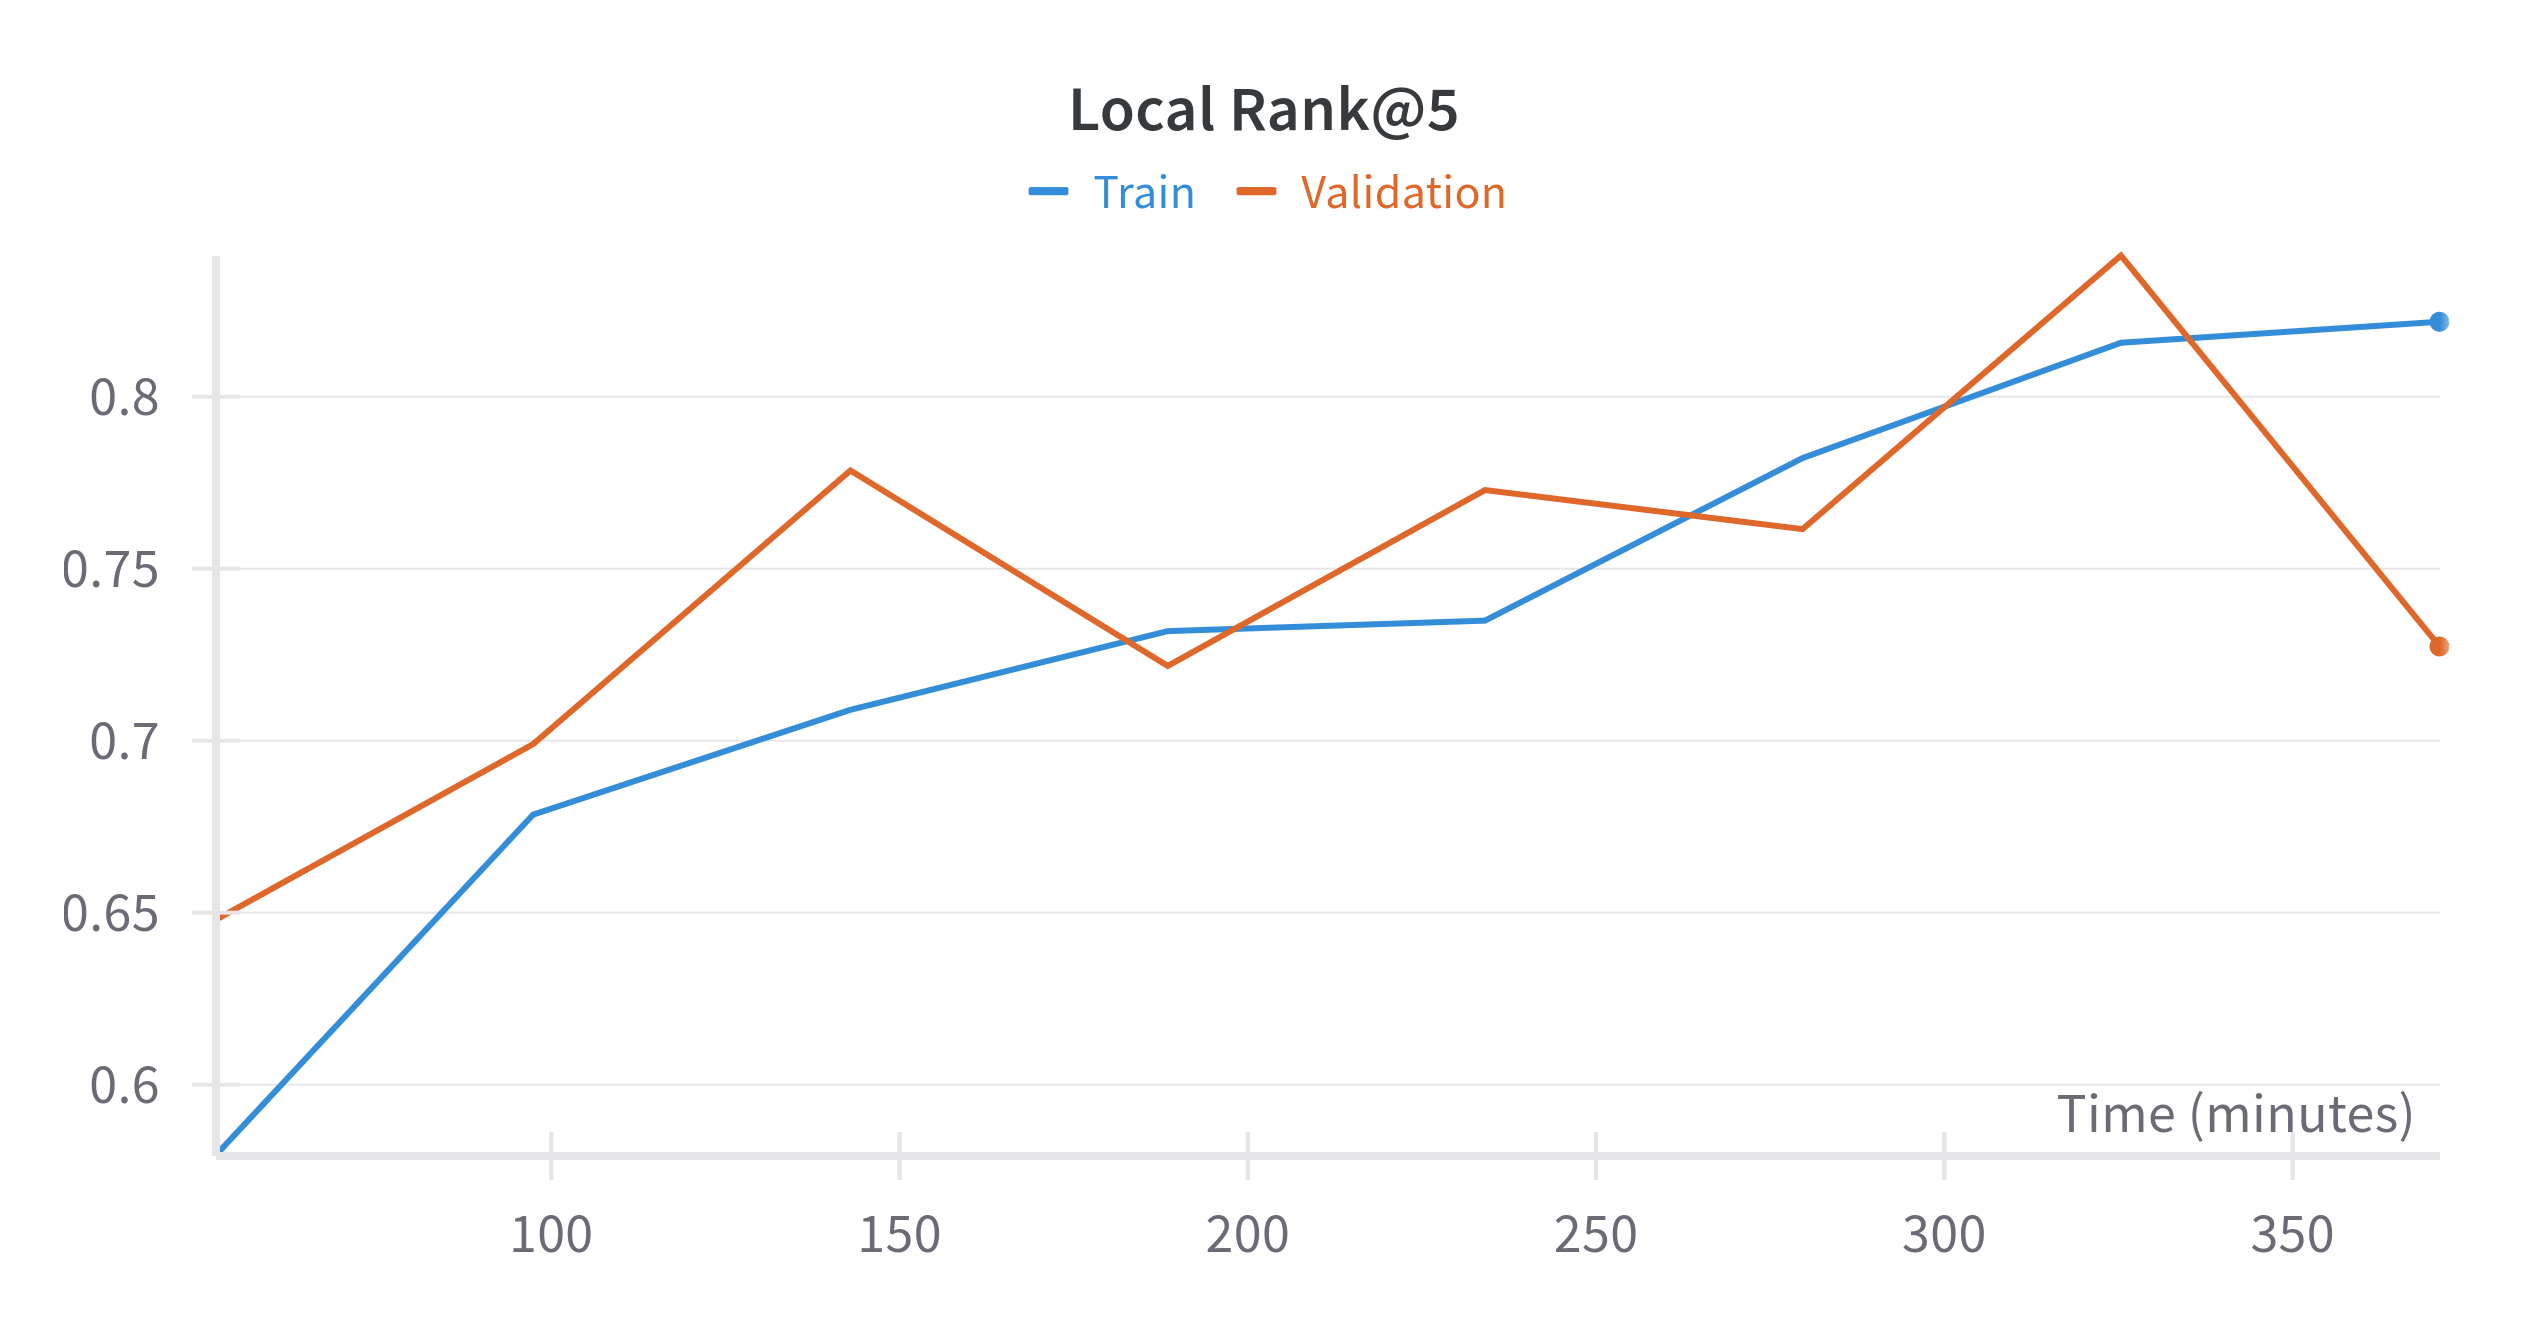
\includegraphics[width=1.0\textwidth]{informatica/wandb/entrenamiento_principal/local_rank@5}
        \caption{\textit{Local Rank@5 Accuracy}}
    \end{subfigure}

    \begin{subfigure}[t]{0.45\textwidth}
        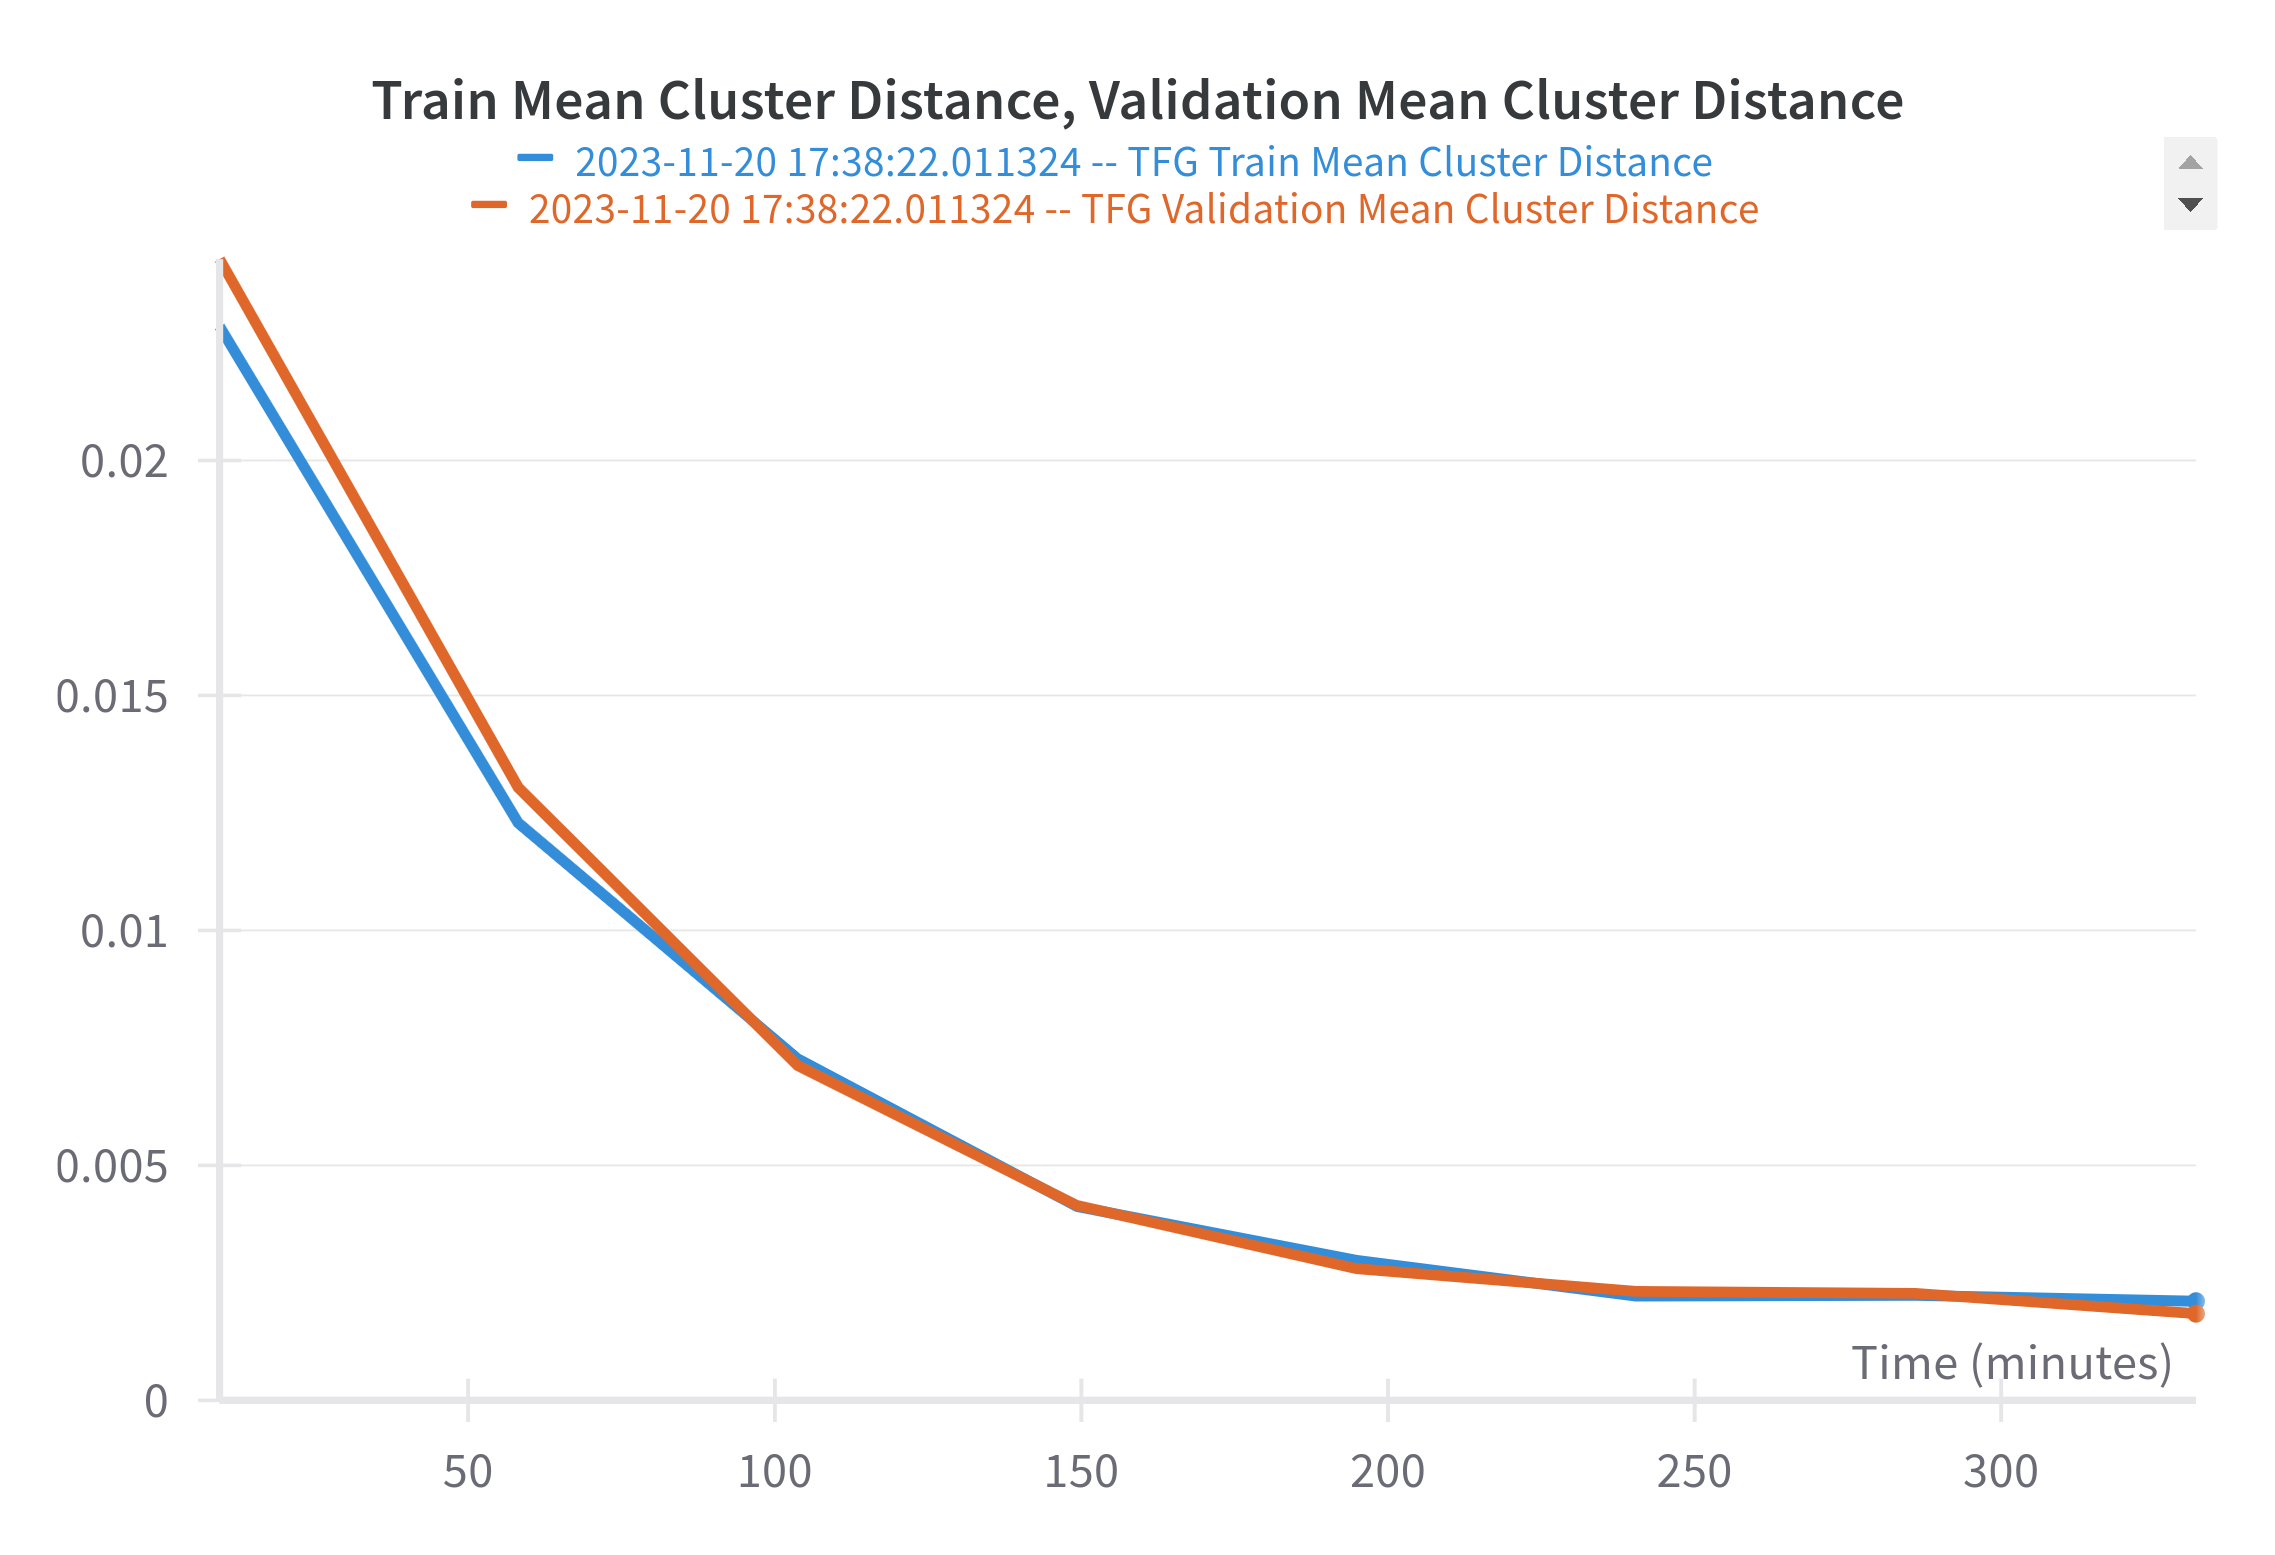
\includegraphics[width=1.0\textwidth]{informatica/wandb/entrenamiento_principal/intracluster_distance}
        \caption{Distanca \textit{intracluster} media}
    \end{subfigure}
    \begin{subfigure}[t]{0.45\textwidth}
        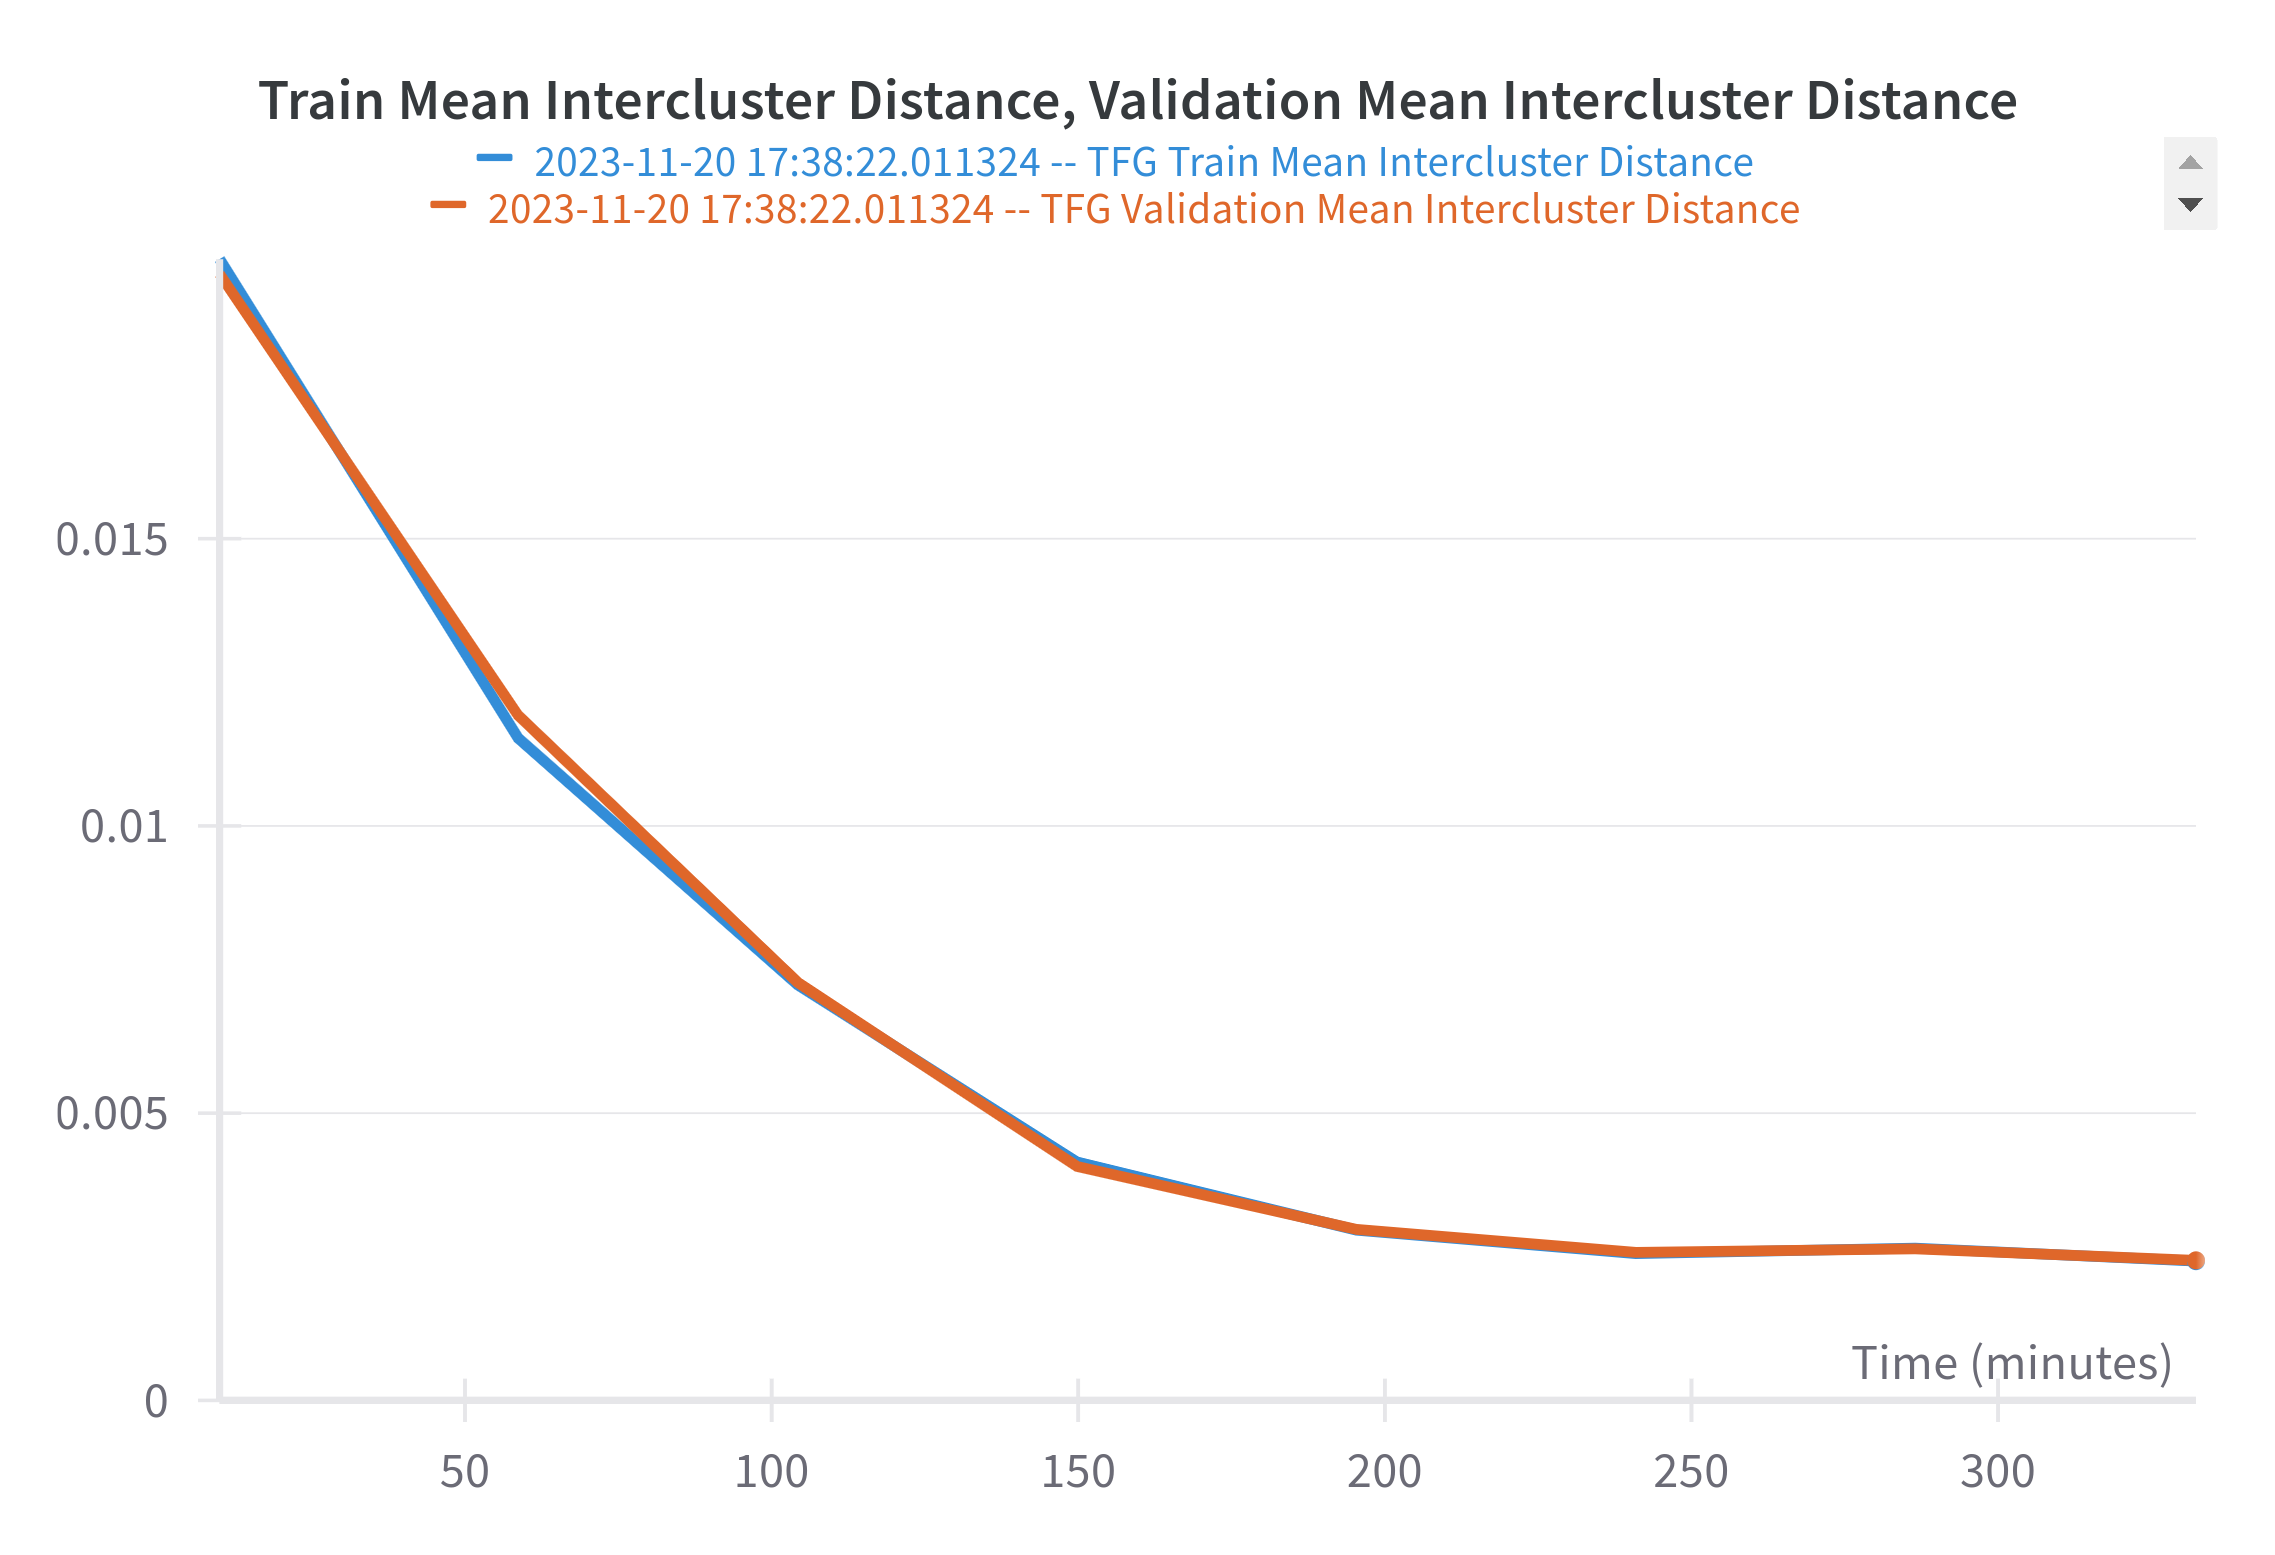
\includegraphics[width=1.0\textwidth]{informatica/wandb/entrenamiento_principal/intercluster_distance}
        \caption{Distancia \textit{intercluster} media}
    \end{subfigure}

    \begin{subfigure}[t]{0.45\textwidth}
        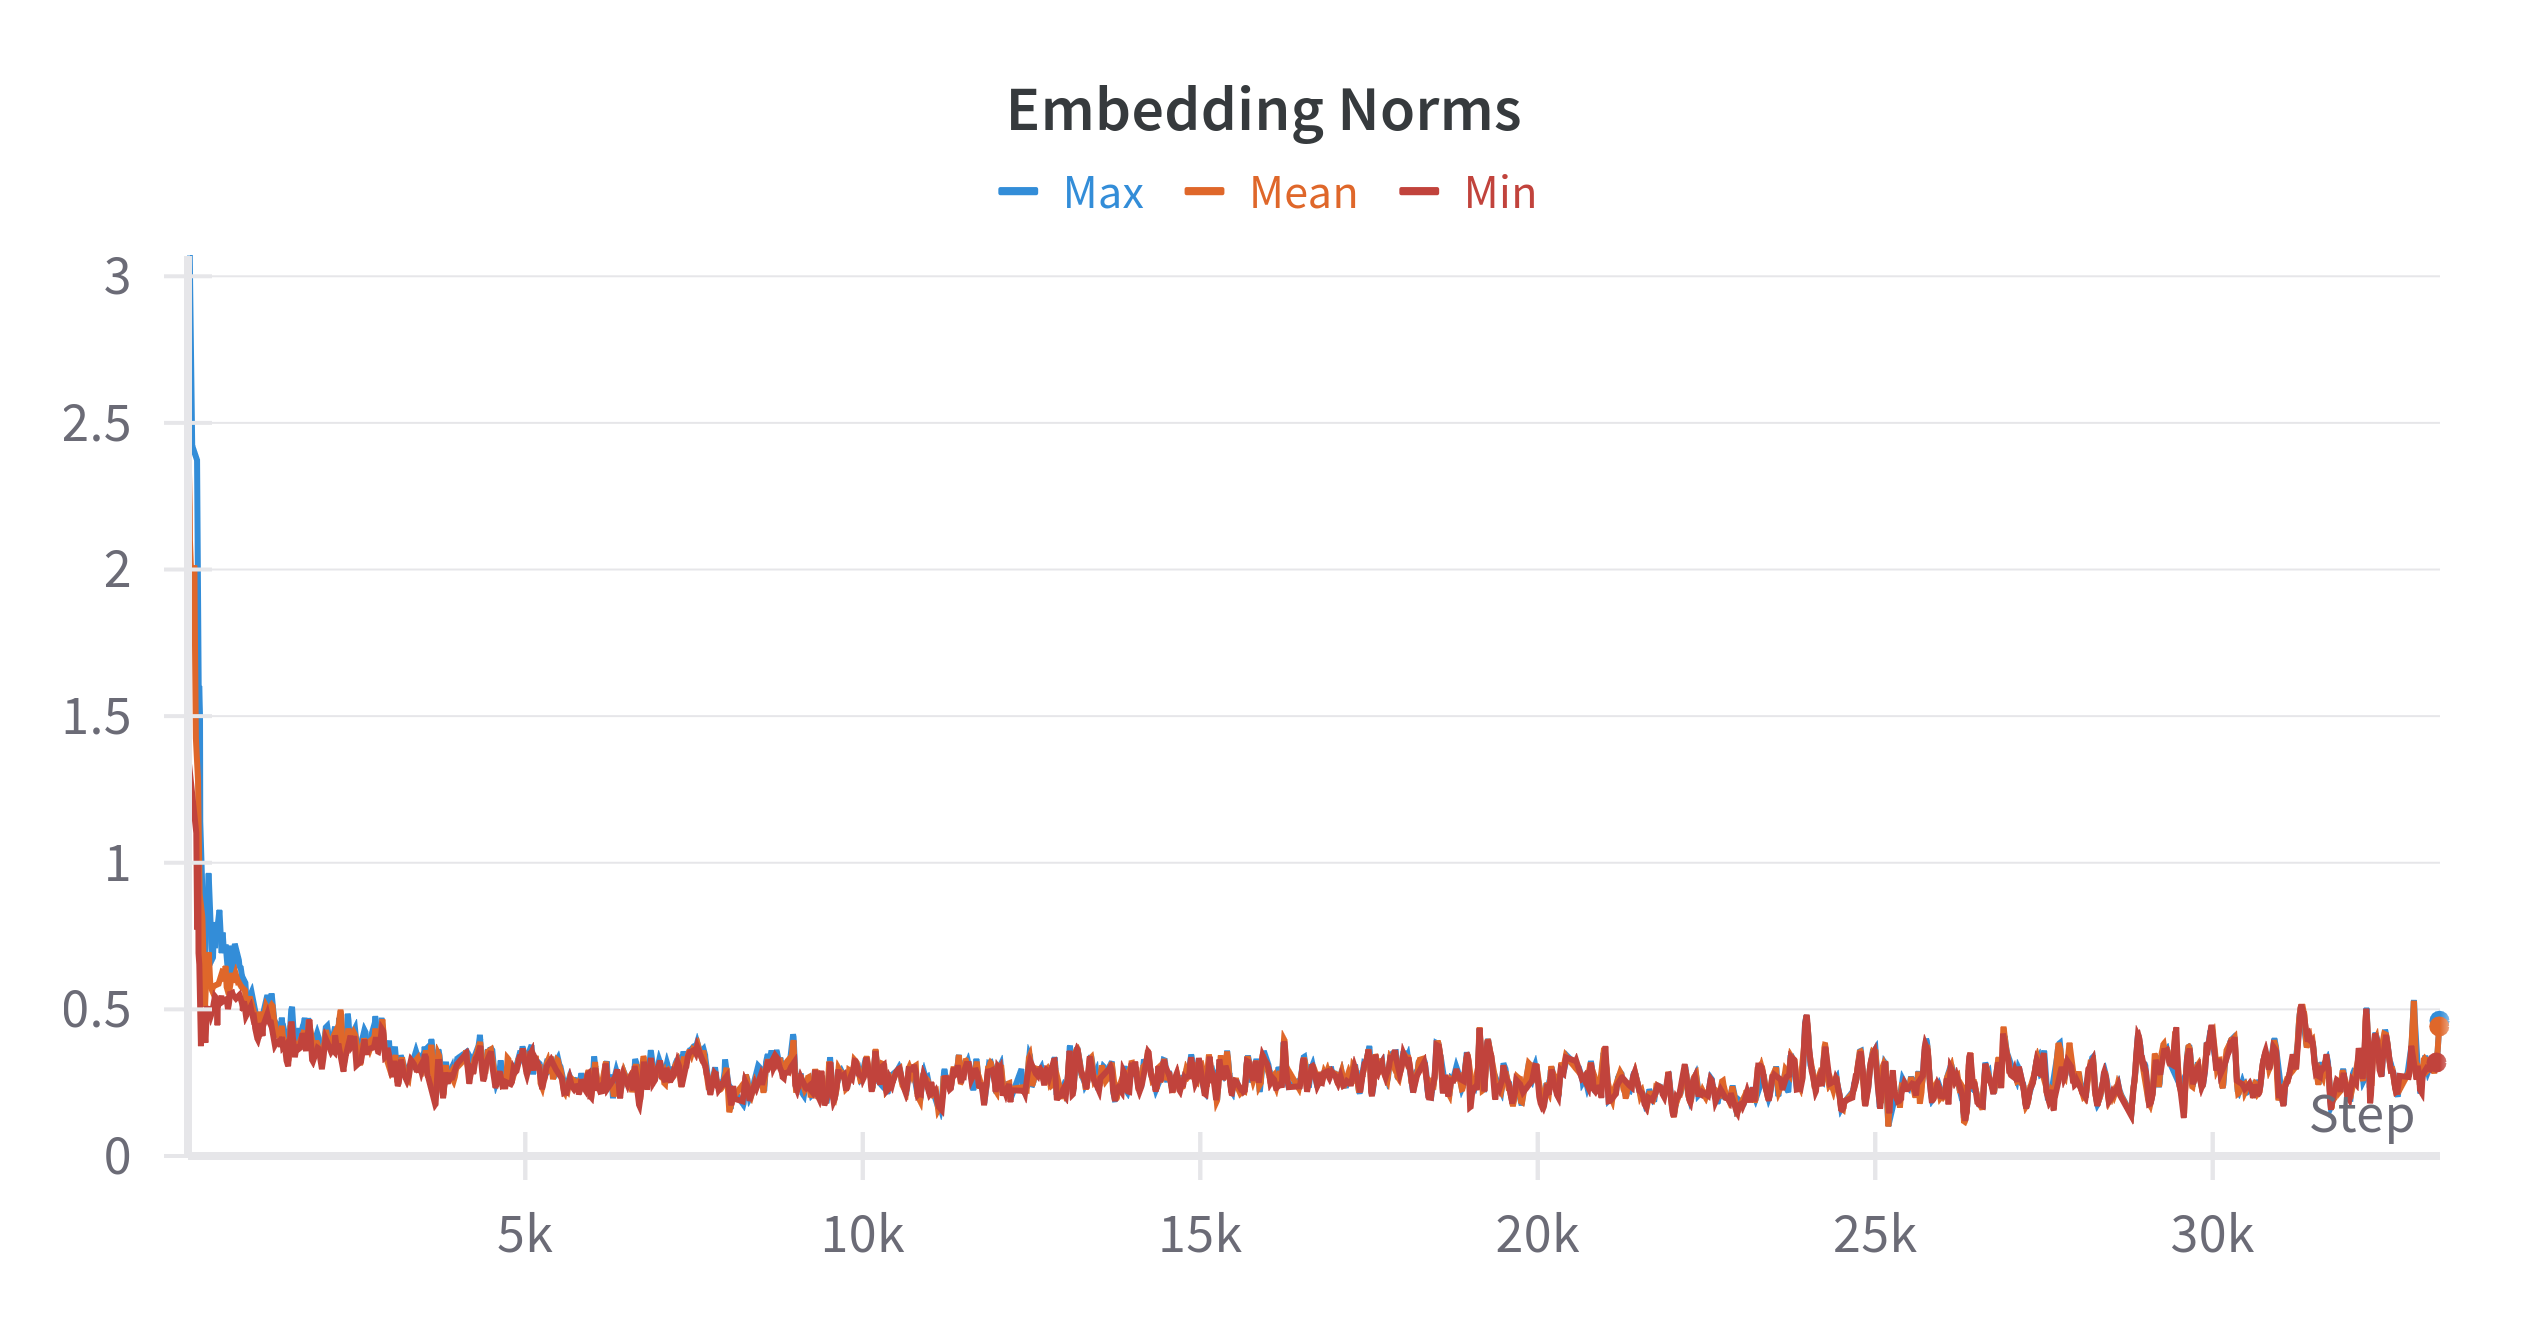
\includegraphics[width=1.0\textwidth]{informatica/wandb/entrenamiento_principal/embedding_norms}
        \caption{Norma de los \textit{embeddings}}
    \end{subfigure}

    \caption{Valores de las métricas observadas durante el proceso de entrenamiento}
    \label{img:metricas_entrenamiento}
\end{figure}

\begin{table}[!hbtp]
\centering
\begin{tabular}{|l|l|l|}
    \hline
    Métrica & Conjunto & Valor \\
    \hline

    \textit{Rank@1 Accuracy} & Entrenamiento & 0.07185 \\
    \textit{Rank@1 Accuracy} & Test & 0.01000 \\
    \textit{Rank@5 Accuracy} & Entrenamiento & 0.15244 \\
    \textit{Rank@5 Accuracy} & Test & 0.00100 \\
    \textit{Silhouette} & Entrenamiento & -0.41858 \\
    \textit{Silhouette} & Test & -0.32984 \\

    \hline

\end{tabular}
\caption{Valores de distintas métricas obtenidas sobre el conjunto \textit{CACD} de entrenamiento y sobre el conjunto \textit{FG-Net} de \textit{test}}
    \label{table:resultados_sobre_fg_net}
\end{table}

A partir de la \imgref{img:metricas_entrenamiento} podemos extraer algunas conclusiones. En primer lugar, observamos que la función de pérdida cae rápidamente mientras que el resto de métricas varían su valor. Esto estaba previsto por lo comentado en \cite{informatica:principal} y, aunque la función de pérdida no varíe, la red puede estar aprendiendo incrementalmente de los datos. En segundo lugar, tanto el \textit{Rank@1} como \textit{Rank@5 Accuracy} aumentan gradualmente, aunque sus valores son realmente bajos. Además, tenemos mejores valores en validación que en entrenamiento, lo que supone un comportamiento inusual que puede indicar que la red no está aprendiendo adecuadamente. Como era de esperar, las dos variantes locales obtienen mejores resultados, pero teniendo en cuenta los valores tan malos de las métricas originales, no podemos fiarnos de estos valores. Finalmente, y quizás lo más importante para saber por qué está fallando este proceso, veamos las distancias intracluster e intercluster. La distancia intracluster desciende hacia cero, como era de esperar. Sin embargo, la distancia intercluster también desciende hacia cero, cuando debería aumentar. Esto va acompañado del hecho de que la norma de los \textit{embeddings} desciende drásticamente al principio del entrenamiento y se mantiene relativamente estable.

Los resultados obtenidos en \tableref{table:resultados_sobre_fg_net} son muy malos. En el conjunto de \textit{CACD} los valores de \textit{Rank@1} y \textit{Rank@5 Accuracy} son pésimos, y están muy lejos de los valores que hemos mostrado que alcanzan modelos estado del arte. Aunque no logremos ser competitivos con el estado del arte, podríamos haber obtenido un modelo aplicable en la práctica, competente y ligero. Pero este no es el caso, en este estado el modelo no es aplicable en ningún escenario. Como es de esperar, los resultados sobre \textit{FG-Net} son aún peores. Todo esto viene reforzado por los valores de la métrica \textit{Silhouette}.

Inicialmente cometemos un error al interpretar estos datos. Pensábamos que el comportamiento del las distancias intracluster e intercluster, acompañado del descenso de la norma de los \textit{embeddings}, era un indicador de la primera fase del entrenamiento que se comenta en \cite{informatica:principal}: agrupamos todos los datos en un cierto centro de gravedad que permite más tarde generar agrupaciones separadas. Para arreglar esto, buscamos mejorar la búsqueda de hiperparámetros y normalizar la salida de las redes. También buscamos aplicar entrenamientos mucho más largos que no mejoran nada. Sin embargo, no nos damos cuenta de un comportamiento muy anómalo. Independientemente del valor del margen que establezcamos, la función de pérdida se queda atascada en este valor. Como comentaremos y justificaremos más tarde, lo que está ocurriendo es que la red aprende el comportamiento degenerado que consiste en transformar todas las entradas a un único punto del espacio vectorial fijo pero no nulo.

\subsection{Experimentación inicial con \textit{MNIST}} \label{isubsec:experimentos_iniciales_mnist}

El primer paso que tomamos para solventar los problemas que se nos presentan es intentar entrenar un modelo sencillo sobre \textit{MNIST}. De esta forma, si obtuviésemos buenos resultados podríamos descartar un posible error por nuestra parte. Y a partir de ahí, buscar ciertas soluciones, como por ejemplo, emplear una arquitectura distinta, probar con una exploración de hiperparámetros más extensa o realizar entrenamientos mucho más extensos.

Como arquitectura usaremos un modelo muy ligero que especificamos en la \tableref{table:arquitectura_mnist}. Validamos esta arquitectura base realizando un entrenamiento para resolver un problema de clasificación clásico, con el que obtenemos más del 95\% de \textit{accuracy} sobre el conjunto de test. Al ser un conjunto de datos tan sencillo no realizamos una exploración de hiperparámetros. Los escogemos a mano realizando ligeros cambios que no cambian sustancialmente los resultados que vamos a mostrar. Finalmente, los hiperparámetros usados y que se corresponden con los resultados que mostramos se exponen en la \tableref{table:hiperparametros_mnist_mal}. El proceso de entrenamiento se puede ver en la \imgref{img:progreso_entrenamiento_mnist_mal} y los resultados en la \tableref{table:resultados_mnist_mal}.

\begin{table}[H]
\centering
\begin{tabular}{|l|l|}
    \hline
    Elemento & Parámetros \\
    \hline
    Convolución & Canales Entrada = 1, Canales Salida = 32, Kernel = 5 \\
    \textit{PreLu} & - \\
    \textit{MaxPool} & Kernel = 2, Stride = 2 \\
    Convolución & Canales Entrada = 32, Canales Salida = 64, Kernel = 5 \\
    \textit{PreLU} & - \\
    \textit{MaxPool} & Kernel = 2, Stride = 2 \\
    Capa densa & Entrada = 1024, Salida = 256 \\
    \textit{PreLU} & - \\
    Capa densa & Entrada = 256, Salida = 256 \\
    \textit{PreLU} & - \\
    Capa densa & Entrada = 256, Salida = tamaño \textit{embedding} \\
    \hline
\end{tabular}
\caption{Descripción de la arquitectura empleada.}
\label{table:arquitectura_mnist}
\end{table}

\begin{table}[!hbtp]
\centering
\begin{tabular}{|l|l|}
    \hline
    Hiperparámetro & Valor \\
    \hline

    P & 16 \\
    K & 8 \\
    $\alpha$ & 1.0 \\
    Función de pérdida & \textit{Batch Hard} \\
    Uso de normalización & No \\
    Dimensión del \textit{embedding} & 5 \\
    \textit{Learning Rate} & 0.001 \\
    Uso de \textit{Softplus} & No \\
    Penalización en la norma de las salidas & No \\
    Épocas de entrenamiento & 20 \\
    \hline
\end{tabular}
\caption{Hiperparámetros empleados para el entrenamiento sobre el cojunto de datos \textit{MNIST}.}
    \label{table:hiperparametros_mnist_mal}
\end{table}

\begin{figure}
\ajustarsubcaptions
\centering
    \begin{subfigure}{.5\textwidth}
        \centering
        \includegraphics[width=0.95\linewidth]{informatica/wandb/experimento_mnist_mal/running_loss.png}
        \caption{Función de pérdida durante el entrenamiento.}
    \end{subfigure}%
    \begin{subfigure}{.5\textwidth}
        \centering
        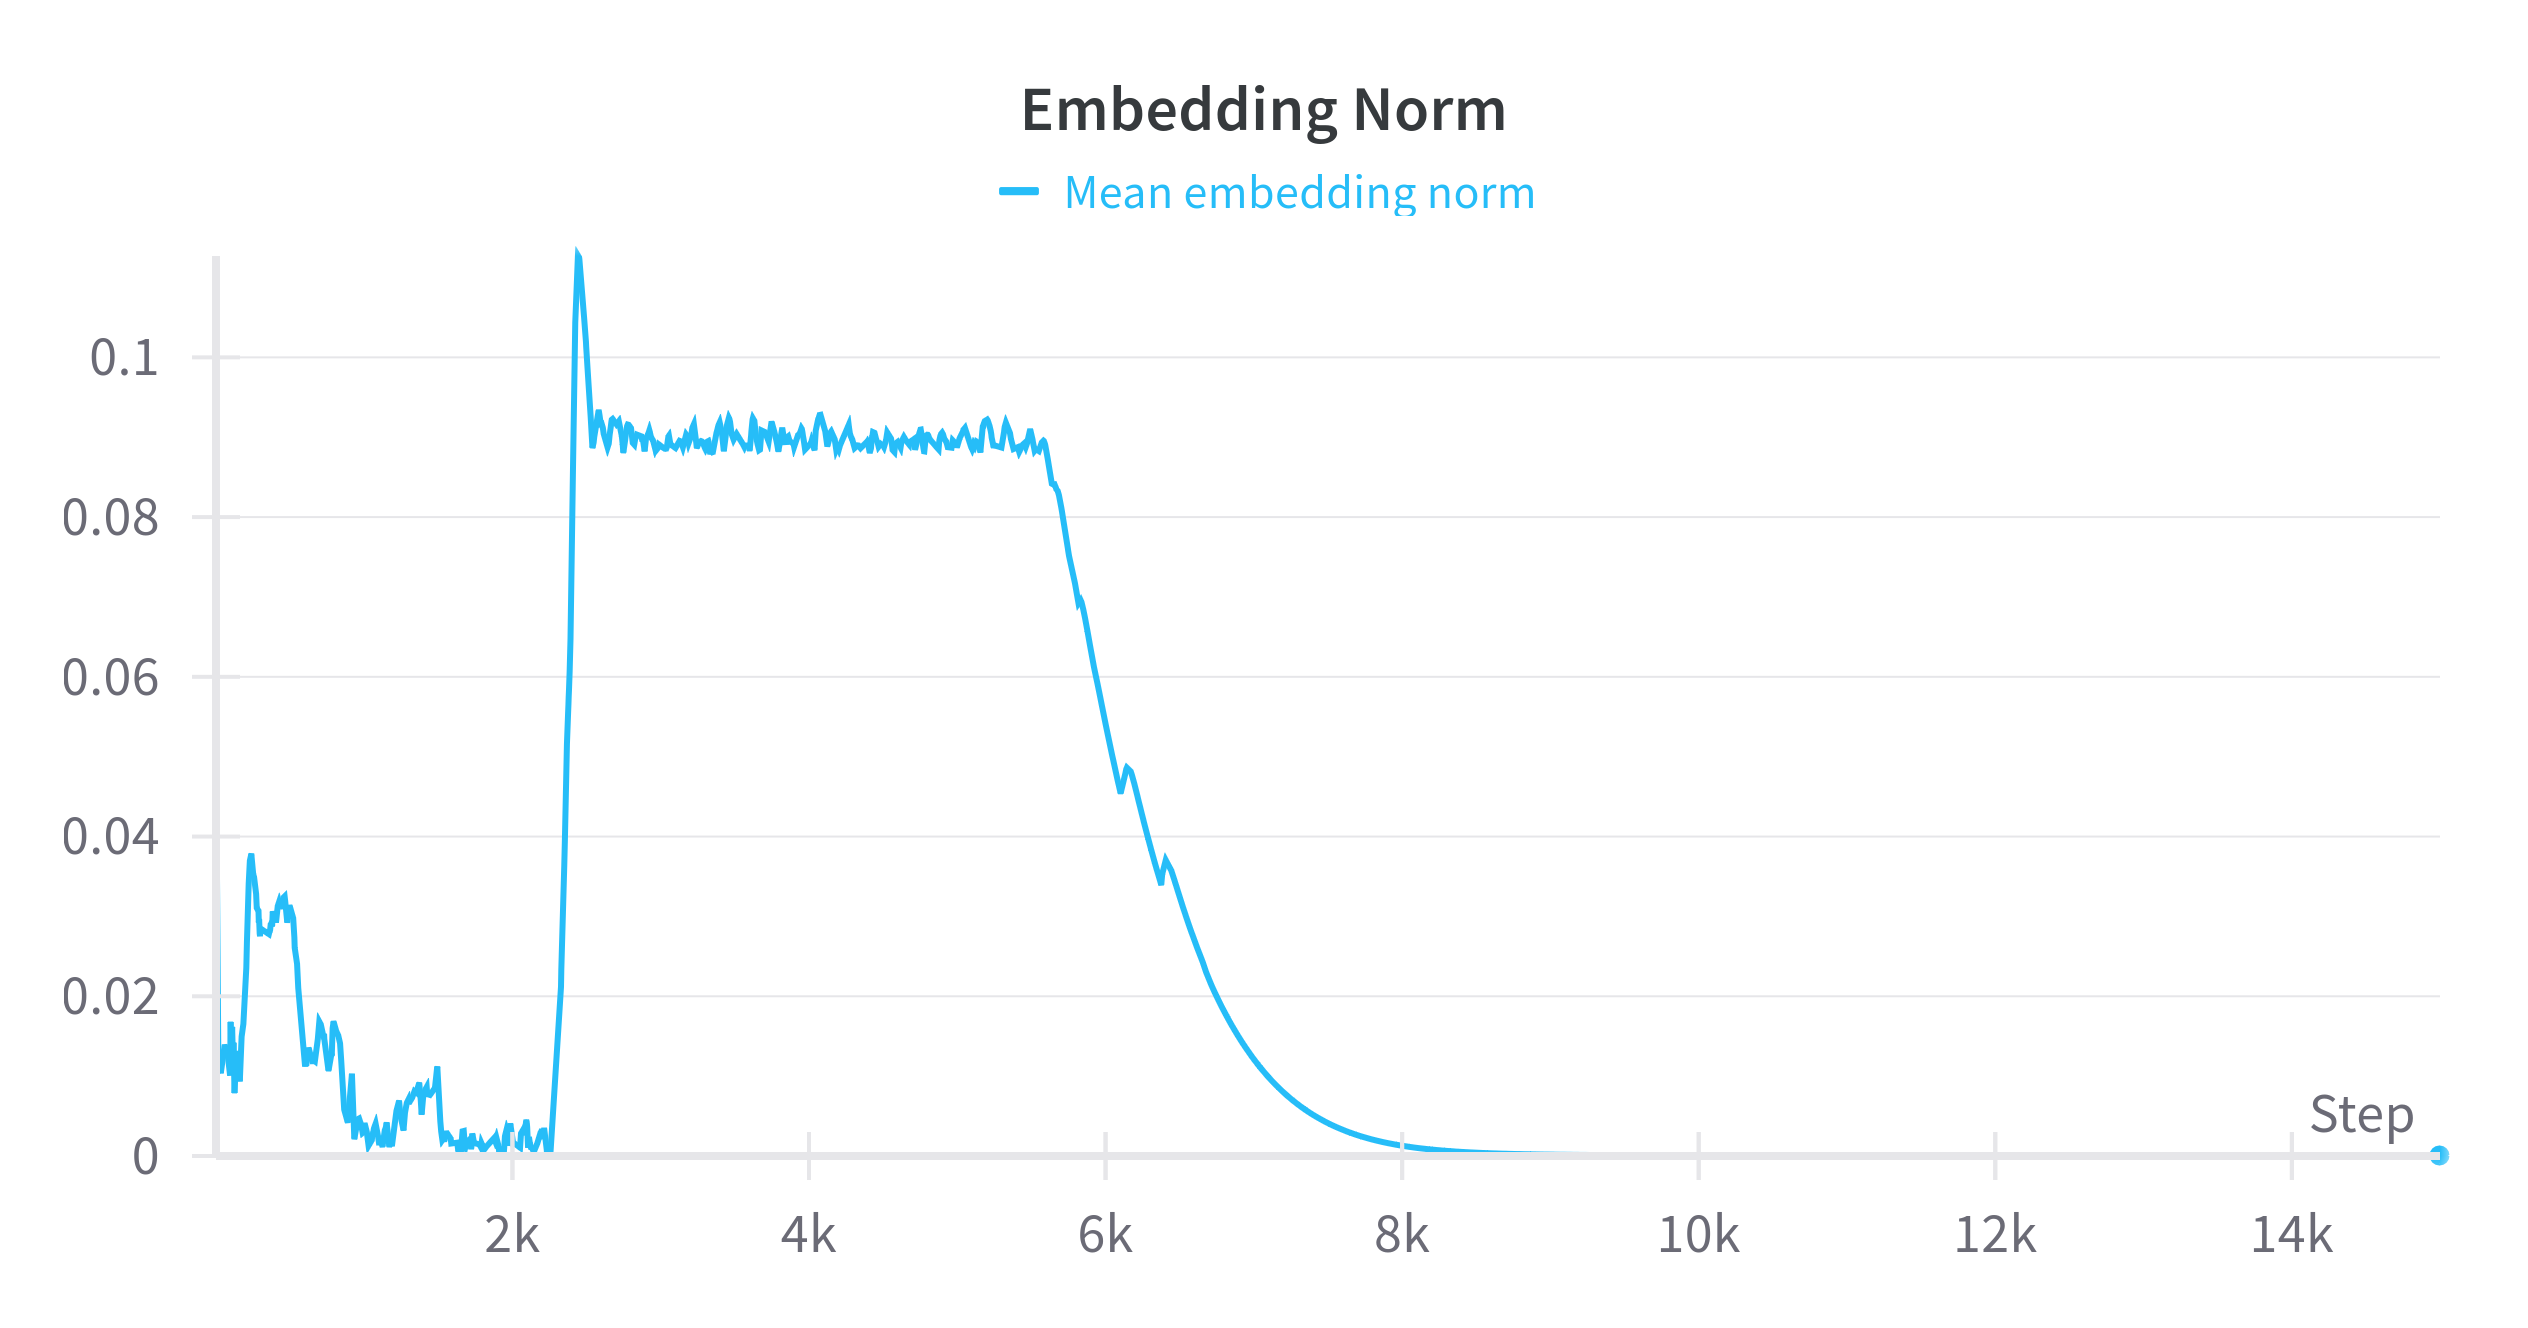
\includegraphics[width=0.95\linewidth]{informatica/wandb/experimento_mnist_mal/embedding_norm.png}
        \caption{Norma de los \textit{embeddings} durante el entrenamiento.}
    \end{subfigure}
    \label{img:progreso_entrenamiento_mnist_mal}
\caption{Métricas observadas durante el entrenamiento.}
\end{figure}

\todo{Introducir las intra inter cluster de las que hablo pero que no he puesto}

\begin{table}[H]
\centering
\begin{tabular}{|l|l|l|l|}
    \hline
    Métrica & Conjunto & Valor \\
    \hline

    \textit{Rank@1 Accuracy} & Entrenamiento & 0.0937 \\
    \textit{Rank@1 Accuracy} & Test & 0.085  \\
    \textit{Rank@5 Accuracy} & Entrenamiento & 0.453  \\
    \textit{Rank@5 Accuracy} & Test & 0.414 \\
    \textit{Silhouette} & Entrenamiento & 0.000 \\
    \textit{Silhouette} & Test & 0.000 \\

    \hline

\end{tabular}
\caption{Métricas de evaluación obtenidas tras entrenar el modelo sobre \textit{MNIST}.}
    \label{table:resultados_mnist_mal}
\end{table}

En la \imgref{img:progreso_entrenamiento_mnist_mal} podemos ver que tenemos exactamente los mismos problemas que en el experimento anterior. La función de pérdida cae rápidamente hasta el valor exacto del margen, quedando estancada en este durante todo el proceso. Cambiando el valor del margen cambiamos el valor exacto en el que la función de pérdida se estanca. Esta vez la norma de los \textit{embeddings} tiene un comportamiento algo distinto. Decrece rápidamente Pero en un punto aumenta drásticamente, se mantiene constante y vuelve a caer hasta cero. Sigue estando lejos de ser el comportamiento que buscamos, una norma que poco a poco aumente. Las distancias intracluster e intercluster siguen teniendo un comportamiento indeseado. Ambas caen rápidamente hacia cero.

Por otro lado, en la \tableref{table:resultados_mnist_mal} podemos ver unos resultados nefastos que siguen la misma línea que el experimento original. Estos son aún menos defendibles al estar trabajando sobre \textit{MNIST}, conjunto de datos sobre el que es muy fácil obtener resultados excelentes. Por lo tanto nos planteamos dos opciones. La primera, que hayamos cometido un error o bien en la implementación de las distintas técnicas o bien en la ejecución de estas. La segunda, que exista algún problema de diseño al aplicar las dos variantes \textit{online} sobre la función de pérdida \textit{Triplet Loss}. El siguiente experimento nos servirá para descartar la primera posibilidad antes de intentar encontrar un fallo de diseño.

\subsection{Experimentación usando otras bases de código para confirmar los problemas de diseño} \label{isubsec:experiemntacion_base_codigo_externa}

Buscamos confirmar que existe un problema en el diseño de las técnicas que estamos empleando, es decir, que usar las variantes \textit{Batch Hard} y \textit{Batch All} sobre \textit{Triplet Loss} produce resultados nefastos. Un primer paso es descartar posibles fallos en la implementación o ejecución de estas técnicas por nuestra parte. Para ello, hemos desarrollado un extenso conjunto de pruebas para validar nuestras implementaciones, como hemos explicado en la \sectionref{isec:test_suite}. Pero además, estudiaremos los experimentos realizados en \cite{informatica:adambielski_github} para confirmar estos problemas.

En el repositorio de \textit{Github} \cite{informatica:adambielski_github} disponemos de dos experimentos, uno sobre \textit{MNIST} y otro sobre \textit{Fashion-MNIST}. Nos centraremos en los experimentos realizados sobre \textit{MNIST}. El autor realiza los siguientes experimentos:

\begin{itemize}
    \item Entrenar usando un enfoque directo, sin \textit{embeddings}, que emplea como \textit{baseline}.
    \item Entrenar usando \textit{contrastive loss}, tanto de forma \textit{offline} como \textit{online}.
    \item Entrenar usando \textit{triplet loss} con minado \textit{offline}.
    \item Entrenar usando \textit{triplet loss} con minado \textit{online} a partir de triples aleatorios.
\end{itemize}

Cabe destacar que el autor ha implementado la estrategia \textit{Batch Hard} y una variante de esta a la que llama \textit{Batch SemiHard}. A pesar de esto, no las muestra en su experimentación, lo que parece indicar que está enfrentándose a los mismos problemas que nosotros. Por lo tanto, adaptamos su código para utilizar estas dos estrategias con su implementación. Al estar usando su base de código, no observamos tantas métricas como en experimentos previos, pero esto no va a suponer un problema pues los resultados van a ser muy interpretables.

Comencemos estudiando la experimentación sobre \textit{Batch Hard}. Usamos la misma arquitectura que en \sectionref{isubsec:experimentos_iniciales_mnist} y que hemos especificado en \tableref{table:arquitectura_mnist}. De hecho, la arquitectura es original de este autor y la hemos replicado en el anterior experimento para que sea más fácil realizar comparaciones entre ambos. Los hiperparámetros empleados se muestran en la \tableref{table:hp_adam_mnist}. El proceso de entrenamiento se pueden observar en la \imgref{img:proceso_entrenamiento_adam_mnist} y, finalmente, los resultados obtenidos se recogen en la \tableref{table:resultados_adam_mnist}.

\begin{table}[!hbtp]
\centering
\begin{tabular}{|l|l|}
    \hline
    Hiperparámetro & Valor \\
    \hline

    P & 16 \\
    K & 8 \\
    $\alpha$ & 1.0 \\
    Función de pérdida & \textit{Batch Hard} \\
    Dimensión del \textit{embedding} & 2 \\
    \textit{Learning Rate} & 0.001 \\
    Épocas de entrenamiento & 20 \\
    \hline
\end{tabular}
    \caption{Hiperparámetros empleados para el entrenamiento sobre el cojunto de datos \textit{MNIST} con la base de código \cite{informatica:adambielski_github}. Algunos hiperparámetros los impone la base de código, como la dimensión del \textit{embedding}.}
    \label{table:hp_adam_mnist}
\end{table}

\begin{figure}[!hbtp]
    \centering
    \includegraphics[width=0.8\textwidth]{informatica/wandb/experimento_mnist_adam/running_loss.png}
    \caption{Función de pérdida durante el entrenamiento, usando \textit{Batch Hard}.}
    \label{img:proceso_entrenamiento_adam_mnist}
\end{figure}

\begin{table}[!hbtp]
\centering
\begin{tabular}{|l|l|l|l|}
    \hline
    Métrica & Conjunto & Valor \\
    \hline

    \textit{Rank@1 Accuracy} & Entrenamiento & 0.05 \\
    \textit{Rank@1 Accuracy} & Test & 0.05  \\
    \textit{Rank@5 Accuracy} & Entrenamiento & 0.523  \\
    \textit{Rank@5 Accuracy} & Test & 0.101 \\
    \textit{Silhouette} & Entrenamiento & 0.000 \\
    \textit{Silhouette} & Test & 0.000 \\
    \hline

\end{tabular}
\caption{Métricas de evaluación obtenidas tras entrenar el modelo sobre \textit{MNIST}, usando \textit{Batch Hard}.}
    \label{table:resultados_adam_mnist}
\end{table}

De nuevo, en base a la \imgref{img:proceso_entrenamiento_adam_mnist} y \tableref{table:resultados_adam_mnist}, aseguramos que esta implementación está enfrentando los mismos problemas que nuestra implementación. Con ello, tenemos más confianza en que exista un problema de diseño y no un problema por nuestra parte. De hecho, como esta base de código impone la dimensión del \textit{embedding} a dos para hacer visualizaciones, mostramos esta visualización en la \imgref{img:train_hard_embeddings}. Estas visualizaciones han sido fundamentales para encontrar el motivo del mal comportamiento de todos los experimentos que hemos presentado hasta ahora. El modelo está transformando todas las entradas a dos vectores fijos del espacio, uno de ellos no nulo.

\begin{figure}
\ajustarsubcaptions
\centering
    \begin{subfigure}{.5\textwidth}
        \centering
        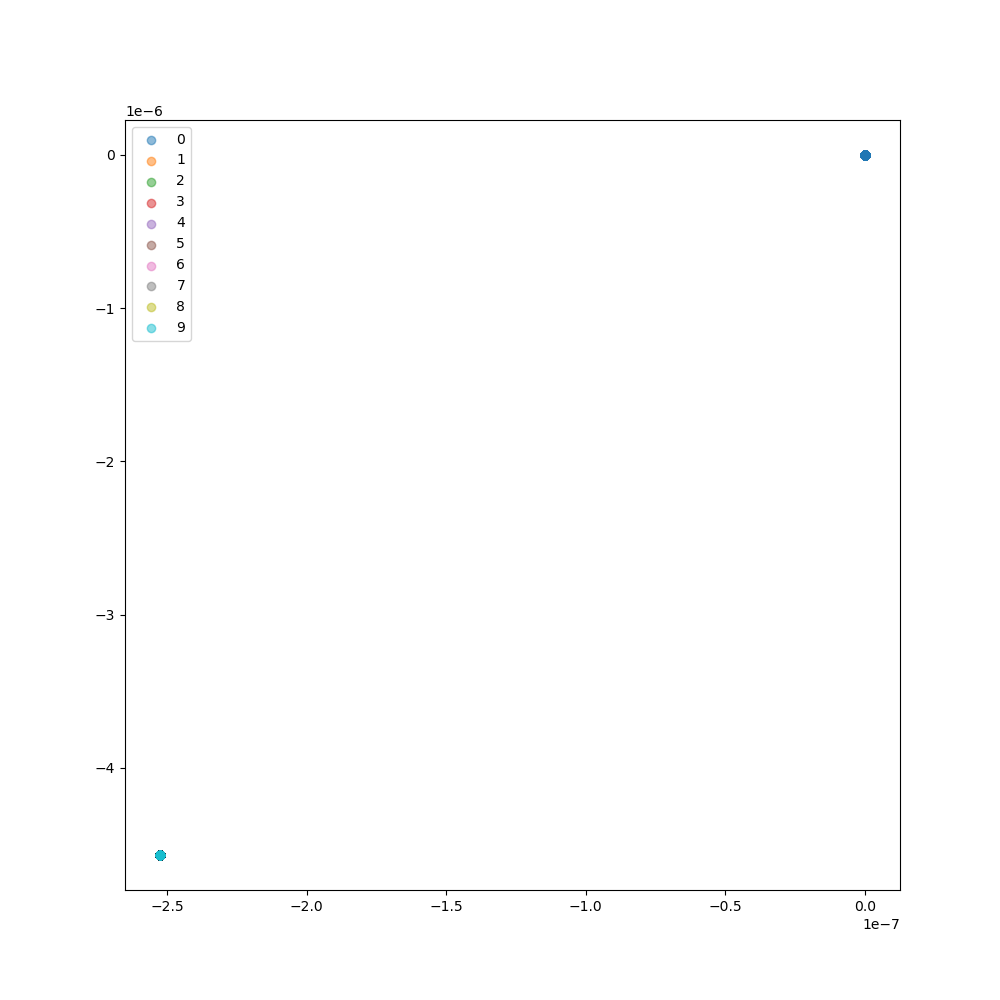
\includegraphics[width=0.8\linewidth]{informatica/wandb/experimento_mnist_adam/hard_train_embedding.png}
        \caption{\textit{Embeddings} aprendidos sobre el conjunto de entrenamiento.}
    \end{subfigure}%
    \begin{subfigure}{.5\textwidth}
        \centering
        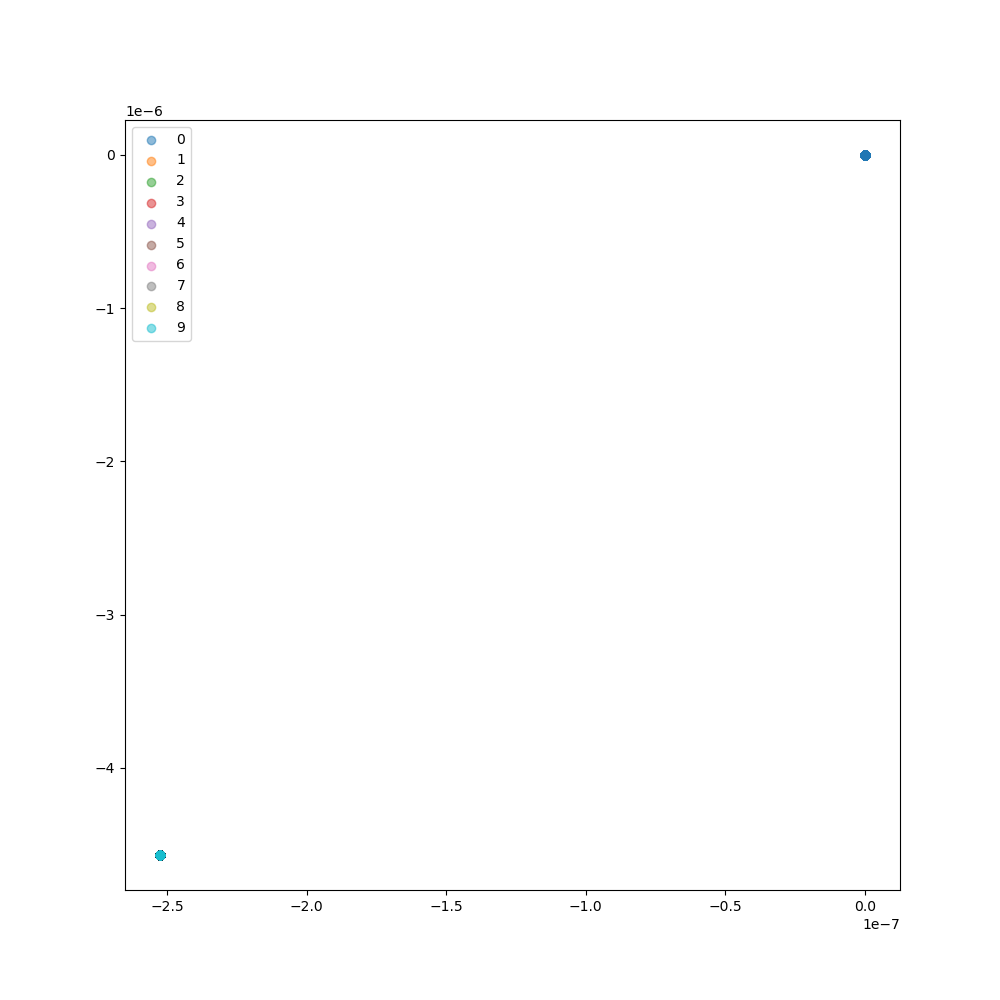
\includegraphics[width=0.8\linewidth]{informatica/wandb/experimento_mnist_adam/hard_test_embedding.png}
        \caption{\textit{Embeddings} aprendidos sobre el conjunto de test.}
    \end{subfigure}
\caption{Visualización de los \textit{embeddings} producidos por el modelo \textit{Batch Hard}. }
\label{img:train_hard_embeddings}
\end{figure}

Veamos ahora los resultados de la técnica \textit{Batch Semihard}. Esta es ligeramente distinta de las dos técnicas que estamos estudiando. En ella, dado un \textit{batch} de $P-K$ elementos, se elige aleatoriamente un triple entre aquellos que tienen un valor de \textit{Triplet Loss} no nulo. Los hiperparámetros serán los mismos que \tableref{table:hp_adam_mnist} salvo por la función de pérdida. El proceso de entrenamiento se muestra en la \imgref{img:proceso_entrenamiento_adam_mnist_random} y los resultados en la \tableref{table:resultados_adam_mnist_random}. Los \textit{embeddings} producidos se visualizan en la \imgref{img:embeddings_adam_random}.

\begin{figure}[!hbtp]
    \centering
    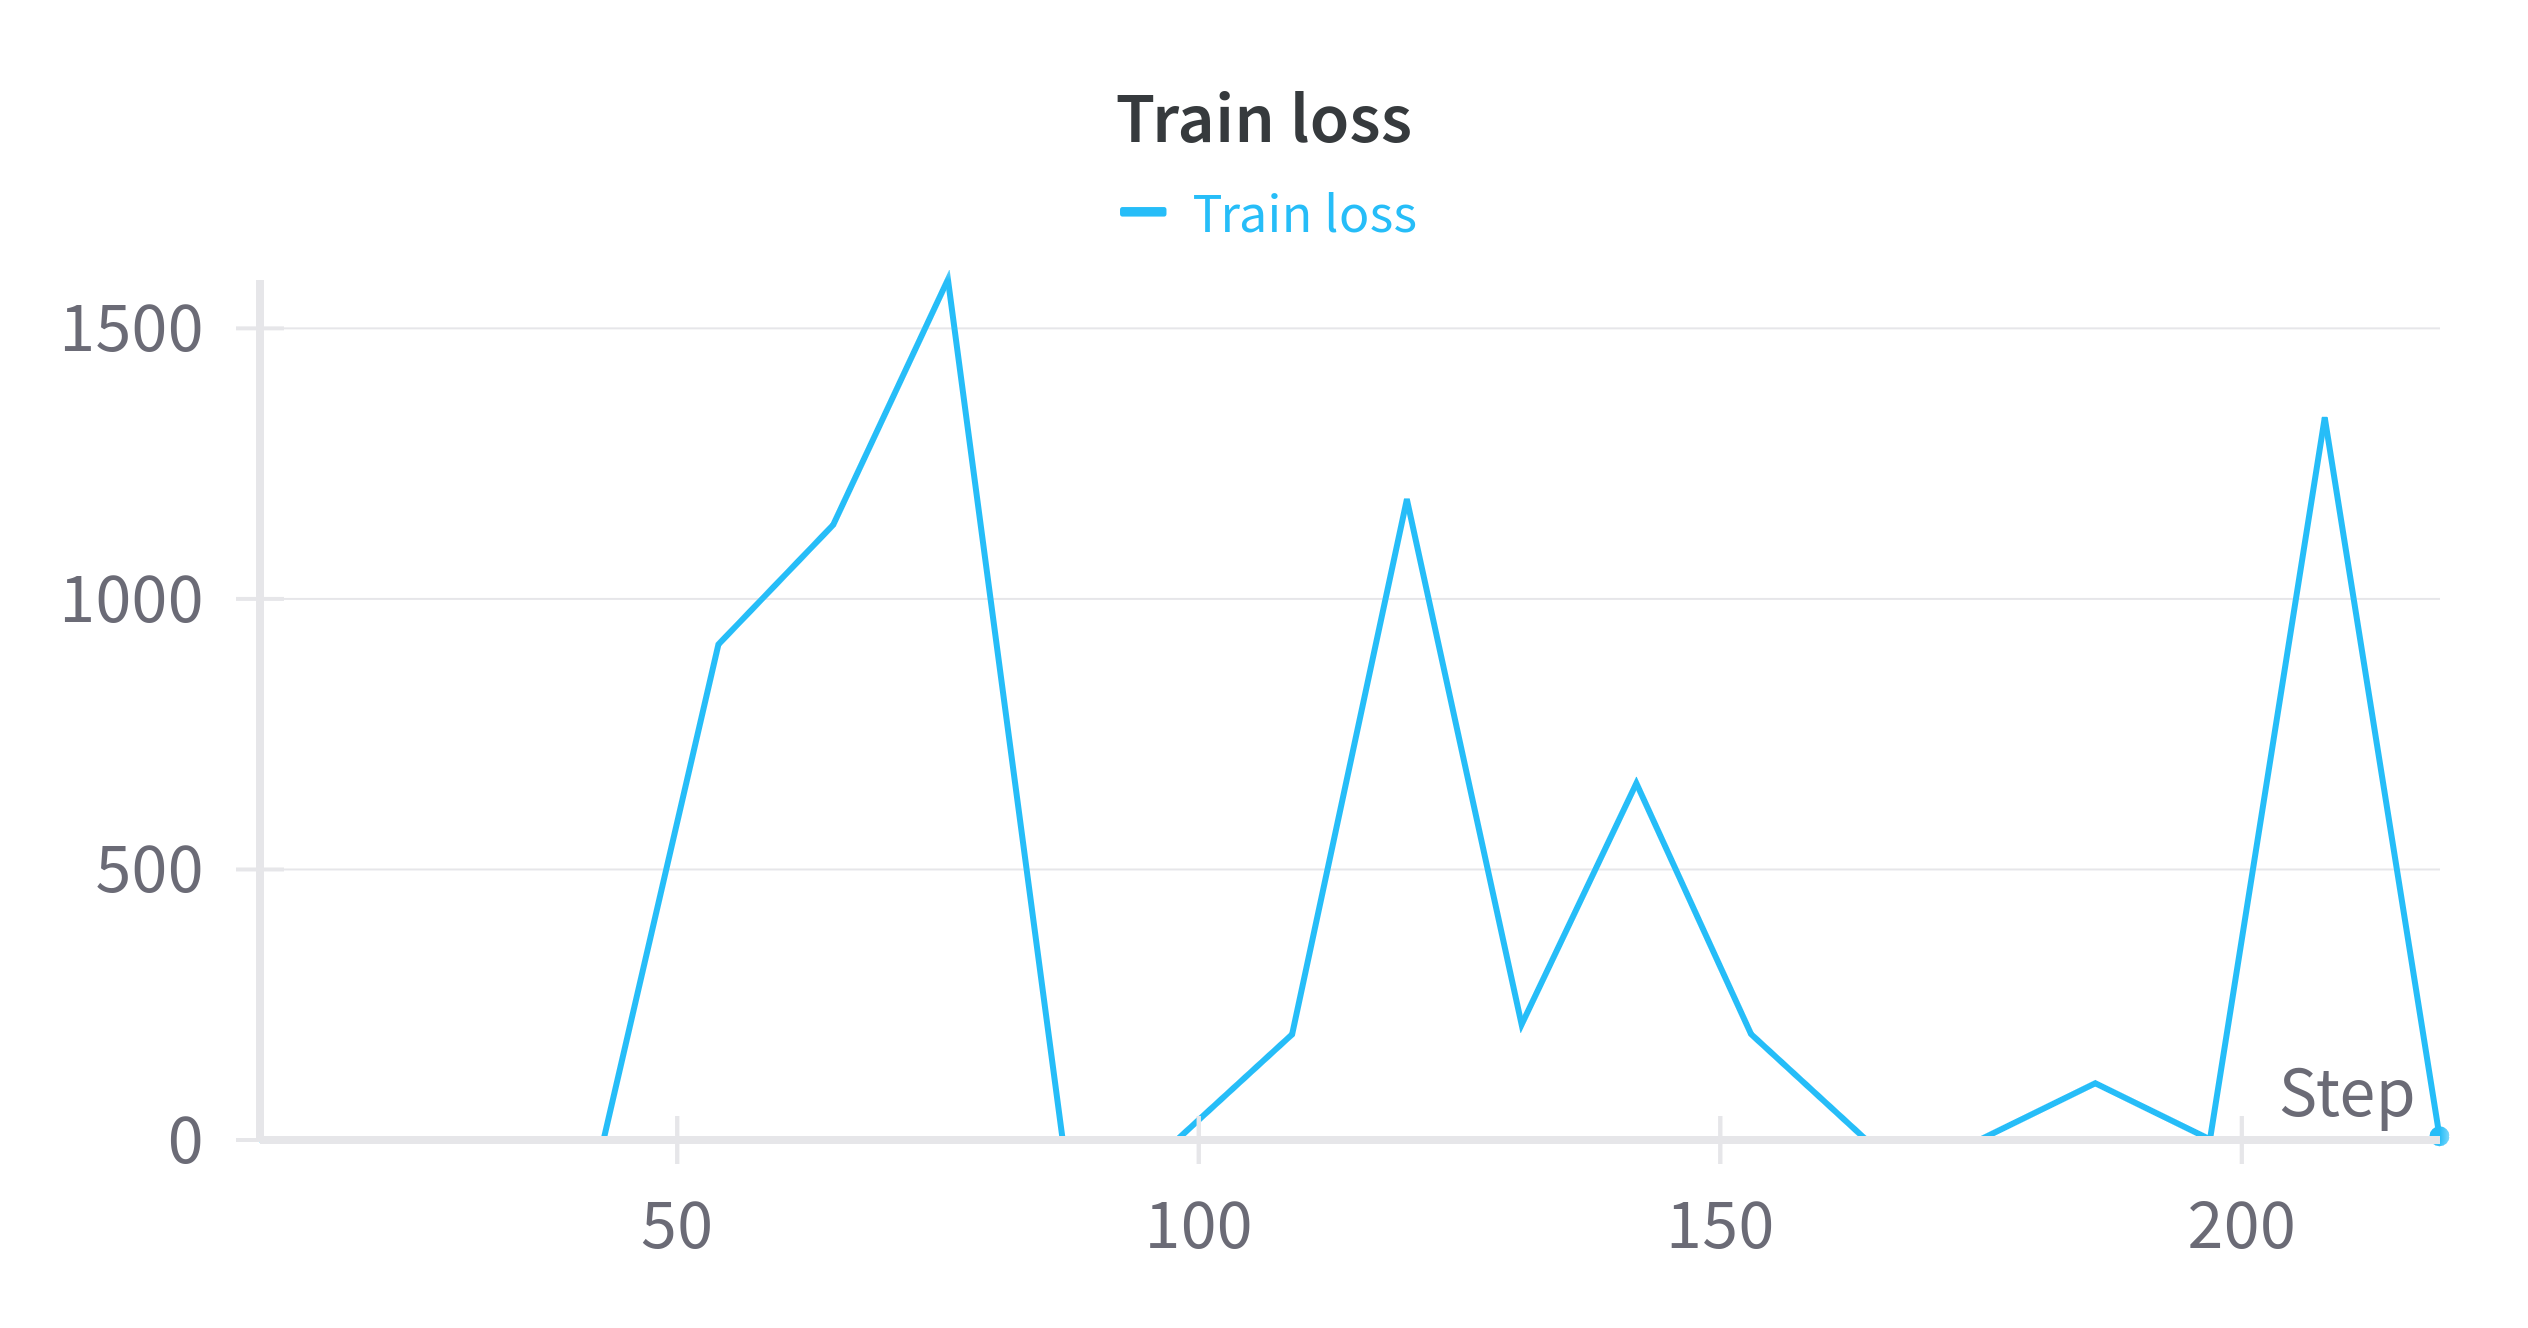
\includegraphics[width=0.8\textwidth]{informatica/wandb/experimento_mnist_adam/running_loss_random.png}
    \caption{Función de pérdida durante el entrenamiento, usando \textit{Batch SemiHard}.}
    \label{img:proceso_entrenamiento_adam_mnist_random}
\end{figure}

\begin{table}[!hbtp]
\centering
\begin{tabular}{|l|l|l|}
    \hline
    Métrica & Conjunto & Valor \\
    \hline

    \textit{Rank@1 Accuracy} & Entrenamiento & 0.916  \\
    \textit{Rank@1 Accuracy} & Test & 0.940  \\
    \textit{Rank@5 Accuracy} & Entrenamiento & 0.980   \\
    \textit{Rank@5 Accuracy} & Test & 0.976  \\
    \textit{Silhouette} & Entrenamiento & 0.648 \\
    \textit{Silhouette} & Test & 0.632 \\
    \hline


\end{tabular}
\caption{Métricas de evaluación obtenidas tras entrenar el modelo sobre \textit{MNIST}, usando \textit{Batch SemiHard}.}
\label{table:resultados_adam_mnist_random}
\end{table}

\begin{figure} [!hbtp]
\ajustarsubcaptions
\centering
    \begin{subfigure}{.5\textwidth}
        \centering
        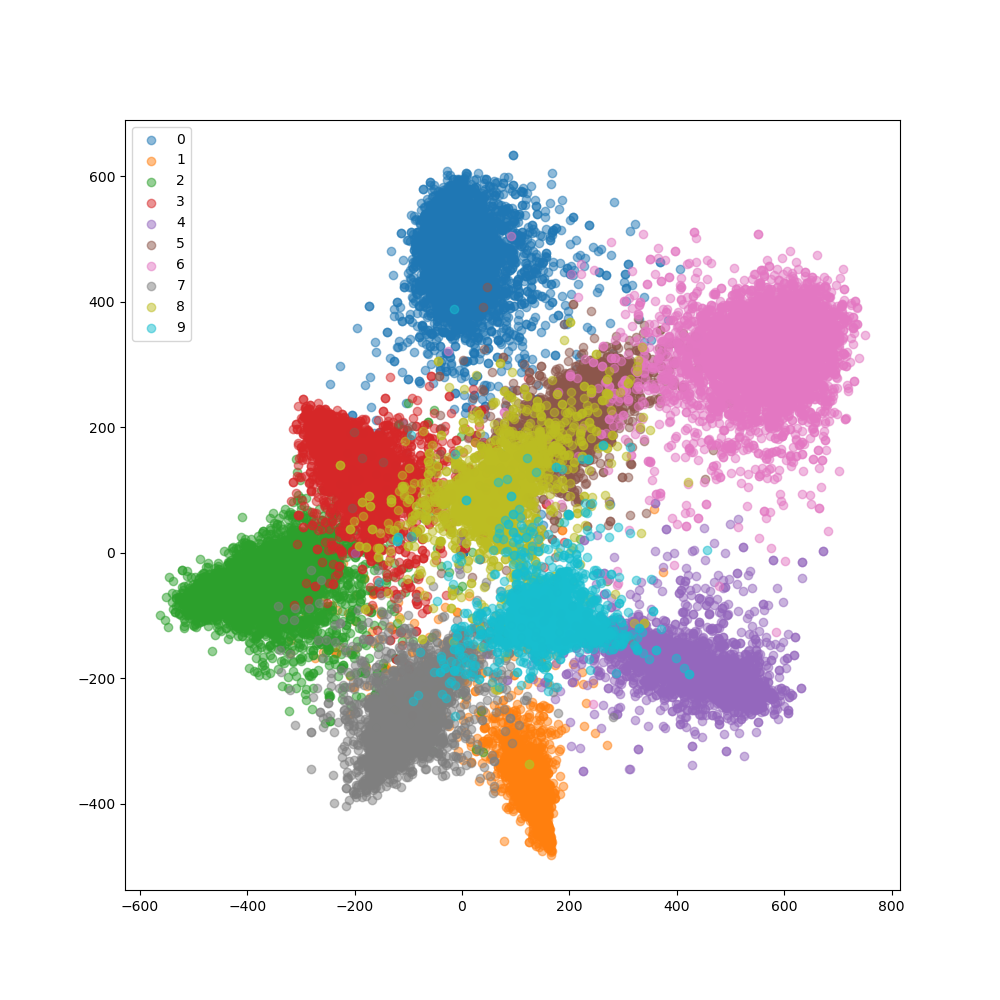
\includegraphics[width=0.8\linewidth]{informatica/wandb/experimento_mnist_adam/random_train_embeddings.png}
        \caption{\textit{Embeddings} aprendidos sobre el conjunto de entrenamiento.}
    \end{subfigure}%
    \begin{subfigure}{.5\textwidth}
        \centering
        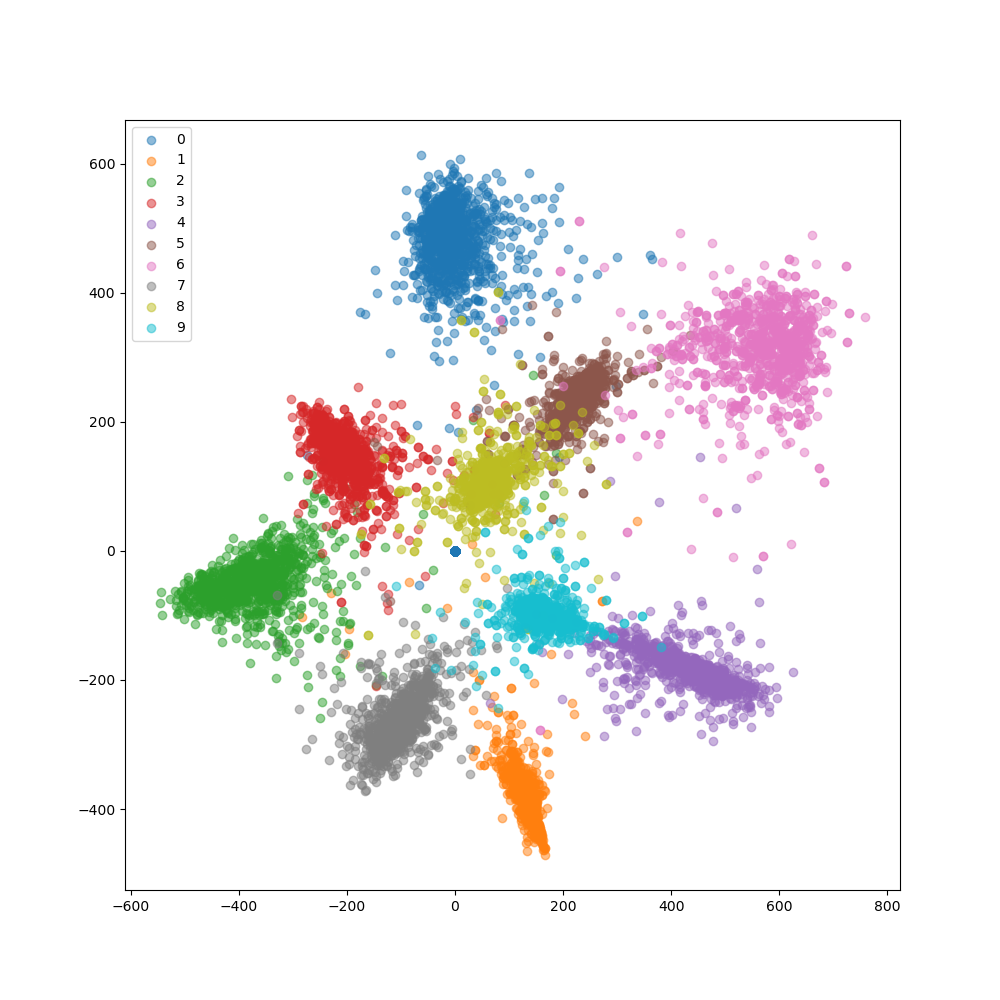
\includegraphics[width=0.8\linewidth]{informatica/wandb/experimento_mnist_adam/random_test_embeddings.png}
        \caption{\textit{Embeddings} aprendidos sobre el conjunto de test.}
    \end{subfigure}
\caption{Visualización de los \textit{embeddings} producidos por el modelo \textit{Batch SemiHard}.}
\label{img:embeddings_adam_random}
\end{figure}

La función de pérdida que observamos en \imgref{img:proceso_entrenamiento_adam_mnist_random} ya no sufre de los problemas que estamos comentando. Aunque tiene una forma algo inusual, alejada de la curva que decrece monótonamente, esta es esperable debido a la fuerte naturaleza aleatoria de la función. Los resultados obtenidos y que mostramos en la \tableref{table:resultados_adam_mnist} ahora sí que están a la altura de la simpleza de \textit{MNIST}. Y para finalizar, los \textit{embeddings} obtenidos en la \imgref{img:embeddings_adam_random} ya no son triviales, se aprecia claramente que el modelo ha aprendido a resolver el problema planteado.

Para finalizar, empleamos el código de \cite{informatica:implementacion_batch_distancias} para calcular las funciones de pérdida y así comprobar por última vez que no tenemos un fallo en nuestra implementación. Repetimos los experimentos tanto para \textit{MNIST} como para \textit{CACD} usando esta nueva implementación, obteniendo exactamente el mismo comportamiento y resultados nefastos. En conclusión, todo indica que existe un fallo en el diseño de las dos técnicas que estamos estudiando, y que los malos resultados no se deben a un fallo de implementación por nuestra parte. Por tanto, deberemos justificar por qué ocurre esto y qué podemos hacer para solventarlo.

\subsection{Detección del problema de diseño y propuesta de una solución} \label{isubsec:identificacion_problemas_propuesta_solucion}

En la \sectionref{isec:triplet_loss} hemos justificado teóricamente por qué es necesario un término $\alpha$ de margen en la función de pérdida: para evitar que la red aprenda el comportamiento degenerado de transformar todas las entradas al vector cero, anulando la función de pérdida. Por otro lado, en \cite{informatica:principal}, se comentan las distintas fases típicas que se desarrollan durante el entrenamiento. En una primera fase todos los \textit{embeddings} de las entradas son atraídos hacia un centro de gravedad. En una segunda fase, los \textit{embeddings} pasan unos por encima de otros a través del centro de gravedad para formar las agrupaciones. Y en la tercera y última fase, las agrupaciones se hacen más compactas y se alejan unas de otras.

El motivo del mal comportamiento se debe a que la red se queda atascada en la primera fase, en un comportamiento degenerado. Aprende a transformar todas las entradas a un vector fijo y no nulo del espacio, el centro de gravedad. Las pequeñas variaciones que necesitamos en la segunda fase pueden hacer que la función de pérdida aumente, por lo que el proceso de entrenamiento no consigue ejecutar satisfactoriamente esta fase. En otros términos, tenemos que la red ha encontrado un centro de gravedad $\nv{v_0} \in \R^M$ de forma que $f(\nv{x}) = \nv{v_0}$, $\forall \nv{x} \in \R^N$, siendo $M$ la dimensión del \textit{embedding} elegida. Así, la función de pérdida verifica que:

\begin{equation} \label{eq:justificacion_relu}
\begin{split}
    \mathcal{L}(a, p, n) &= ReLU(d(a, p) - d(a, n) + \alpha) = ReLU(d(\nv{v_0}, \nv{v_0}) - d(\nv{v_0}, \nv{v_0}) + \alpha) \\
    &= ReLU(0 - 0 + \alpha) = ReLU(\alpha) = \alpha.
\end{split}
\end{equation}

Todos los resultados que hemos presentado hasta ahora se alinean con esta explicación. Tanto en la \imgref{img:metricas_entrenamiento} como en la \imgref{img:progreso_entrenamiento_mnist_mal} se aprecia que la función de pérdida se queda estancada exactamente en el valor del margen. Además, cuando cambiamos este hiperparámetro la función se estanca en este nuevo valor. Este comportamiento tan extraño ha quedado perfectamente explicado por la ecuación \eqref{eq:justificacion_relu}. Adicionalmente, en estas gráficas también podemos apreciar que las distancias intracluster e intercluster tienden a cero, comportamiento que también hemos explicado. La \imgref{img:train_hard_embeddings} termina de respaldar la ecuación \eqref{eq:justificacion_relu}, teniendo en cuenta que el modelo colapsa en dos vectores fijos en vez de en uno único.

Ahora que hemos identificado la raíz del problema, podemos proponer una solución a este. Queremos que las distancias intracluster tiendan a cero y que las intercluster crezcan. Las distancias intercluster las podemos controlar con el término de distancia entre ancla y negativo de la función de pérdida. Por tanto, vamos a penalizar distancias ancla-negativo pequeñas introduciendo un termino correctivo en la función de pérdida. Dado un \textit{batch} de $P-K$ imágenes obtenemos una lista de distancias positivas (distancias entre ancla y positivo) y distancias negativas (distancias entre ancla y negativo). Transformamos la función de pérdida penalizando distancias ancla-negativo pequeñas, dividiendo por la media del \textit{batch}. Consideramos $a, p, n$ como vectores de \textit{embeddings} y funciones $\hat{ReLU}$ y $\hat{d}(\cdot, \cdot)$ vectorizadas en:

\begin{equation}
    \mathcal{L}(a, p, n) = \hat{ReLU}(\hat{d}(a, p) - \hat{d}(a, n) + \alpha)
\end{equation}

Para corregir, consideramos:

\begin{equation}
    \mathcal{L}(a, p, n) = \hat{ReLU}((\hat{d}(a, p) - \hat{d}(a, n)) / mean(d(a, n)) + \alpha)
\end{equation}

\todo{No me convence cómo he expresado estas operaciones}

En este punto nos preguntamos si esta solución es original o si ya ha sido considerada. Buscando una solución al problema de la función de pérdida colapsando en el margen nos encontramos con muchos foros que no proponen esta solución sino otras. De hecho, antes de encontrar la raíz del problema, hemos probado muchas de las soluciones propuestas sin llegar a una solución eficaz. Por ejemplo, en \cite{informatica:respuesta_erronea_problema} se menciona justo este problema pero se proponen otras soluciones alejadas de la corrección de distancias ancla-negativo. En \cite{informatica:github_issue_problema_tripletloss} también se mencionan problemas parecidos con \textit{triplet loss}. Únicamente en \cite{informatica:solucion_triplet_loss} encontramos la identificación del problema y la misma propuesta de solución. Sin embargo, no encontramos literatura científica que mencione o resuelva este problema de esta manera. Por todo esto, consideramos que nuestra propuesta es en cierta medida original.

A continuación repetiremos los experimentos sobre \textit{MNIST} y \textit{CACD} para comprobar la efectividad de nuestra propuesta.

\subsection{Resultados sobre \textit{MNIST} con nuestra propuesta de solución} \label{isubsec:experimentacion_mnist_bien}

Para comparar los resultados antes y después de aplicar la técnica usamos la misma arquitectura (que hemos descrito en la \tableref{table:arquitectura_mnist}) y los mismos hiperparámetros (que hemos especificado en la \tableref{table:hiperparametros_mnist_mal}), con la salvedad de que estamos ejecutando dos experimentos, uno para \textit{Batch Hard} y otro para \textit{Batch All}. Los dos procesos de entrenamiento se pueden estudiar en la \imgref{img:procesos_entrenamiento_mnist_corregido}. Los resultados obtenidos con ambas técnicas corregidas se muestra en la \tableref{table:resultados_mnist_corregido}. Finalmente, los \textit{embeddings} producidos sobre el conjunto de \textit{test} se muestran en la \imgref{img:mnist_corregido_embeddings_aprendidos}.

\begin{figure}[!hbtp]
    \centering
    \begin{subfigure}{.5\textwidth}
        \centering
        \includegraphics[width=0.8\linewidth]{informatica/wandb/mnist_corregido/batch_hard_running_loss.png}
        \caption{Función de pérdida.}
    \end{subfigure}%
    \begin{subfigure}{.5\textwidth}
        \centering
        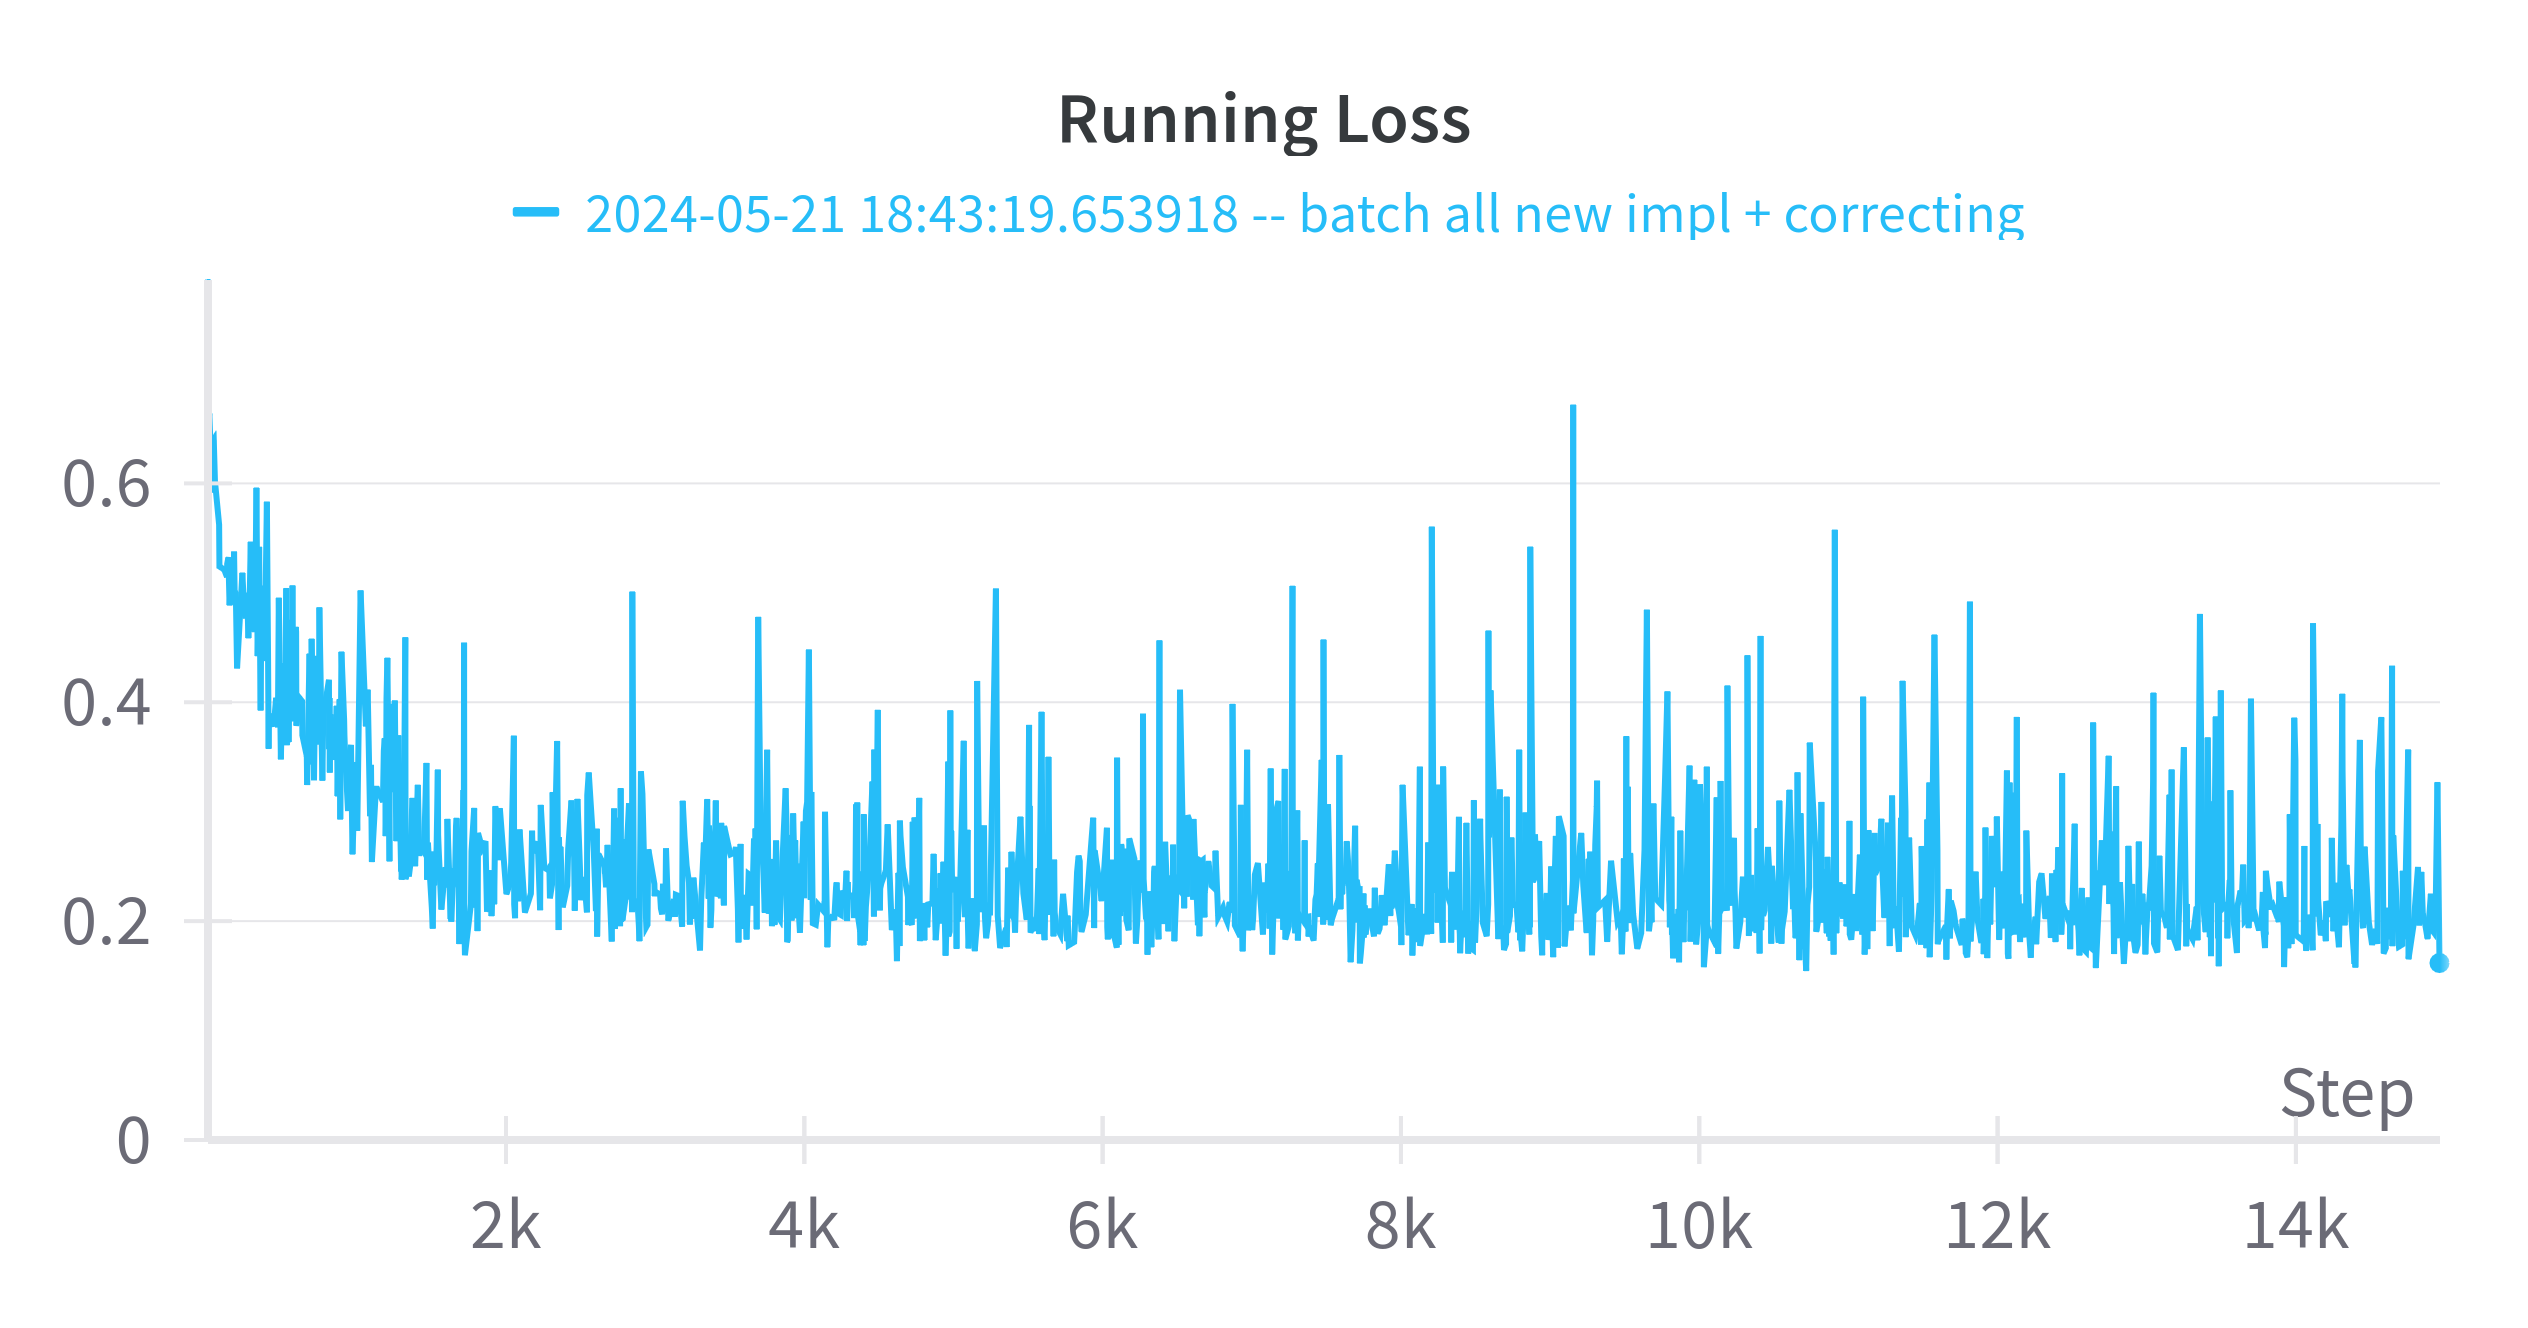
\includegraphics[width=0.8\linewidth]{informatica/wandb/mnist_corregido/bath_all_running_loss.png}
        \caption{Función de pérdida.}
    \end{subfigure}

    \begin{subfigure}{.5\textwidth}
        \centering
        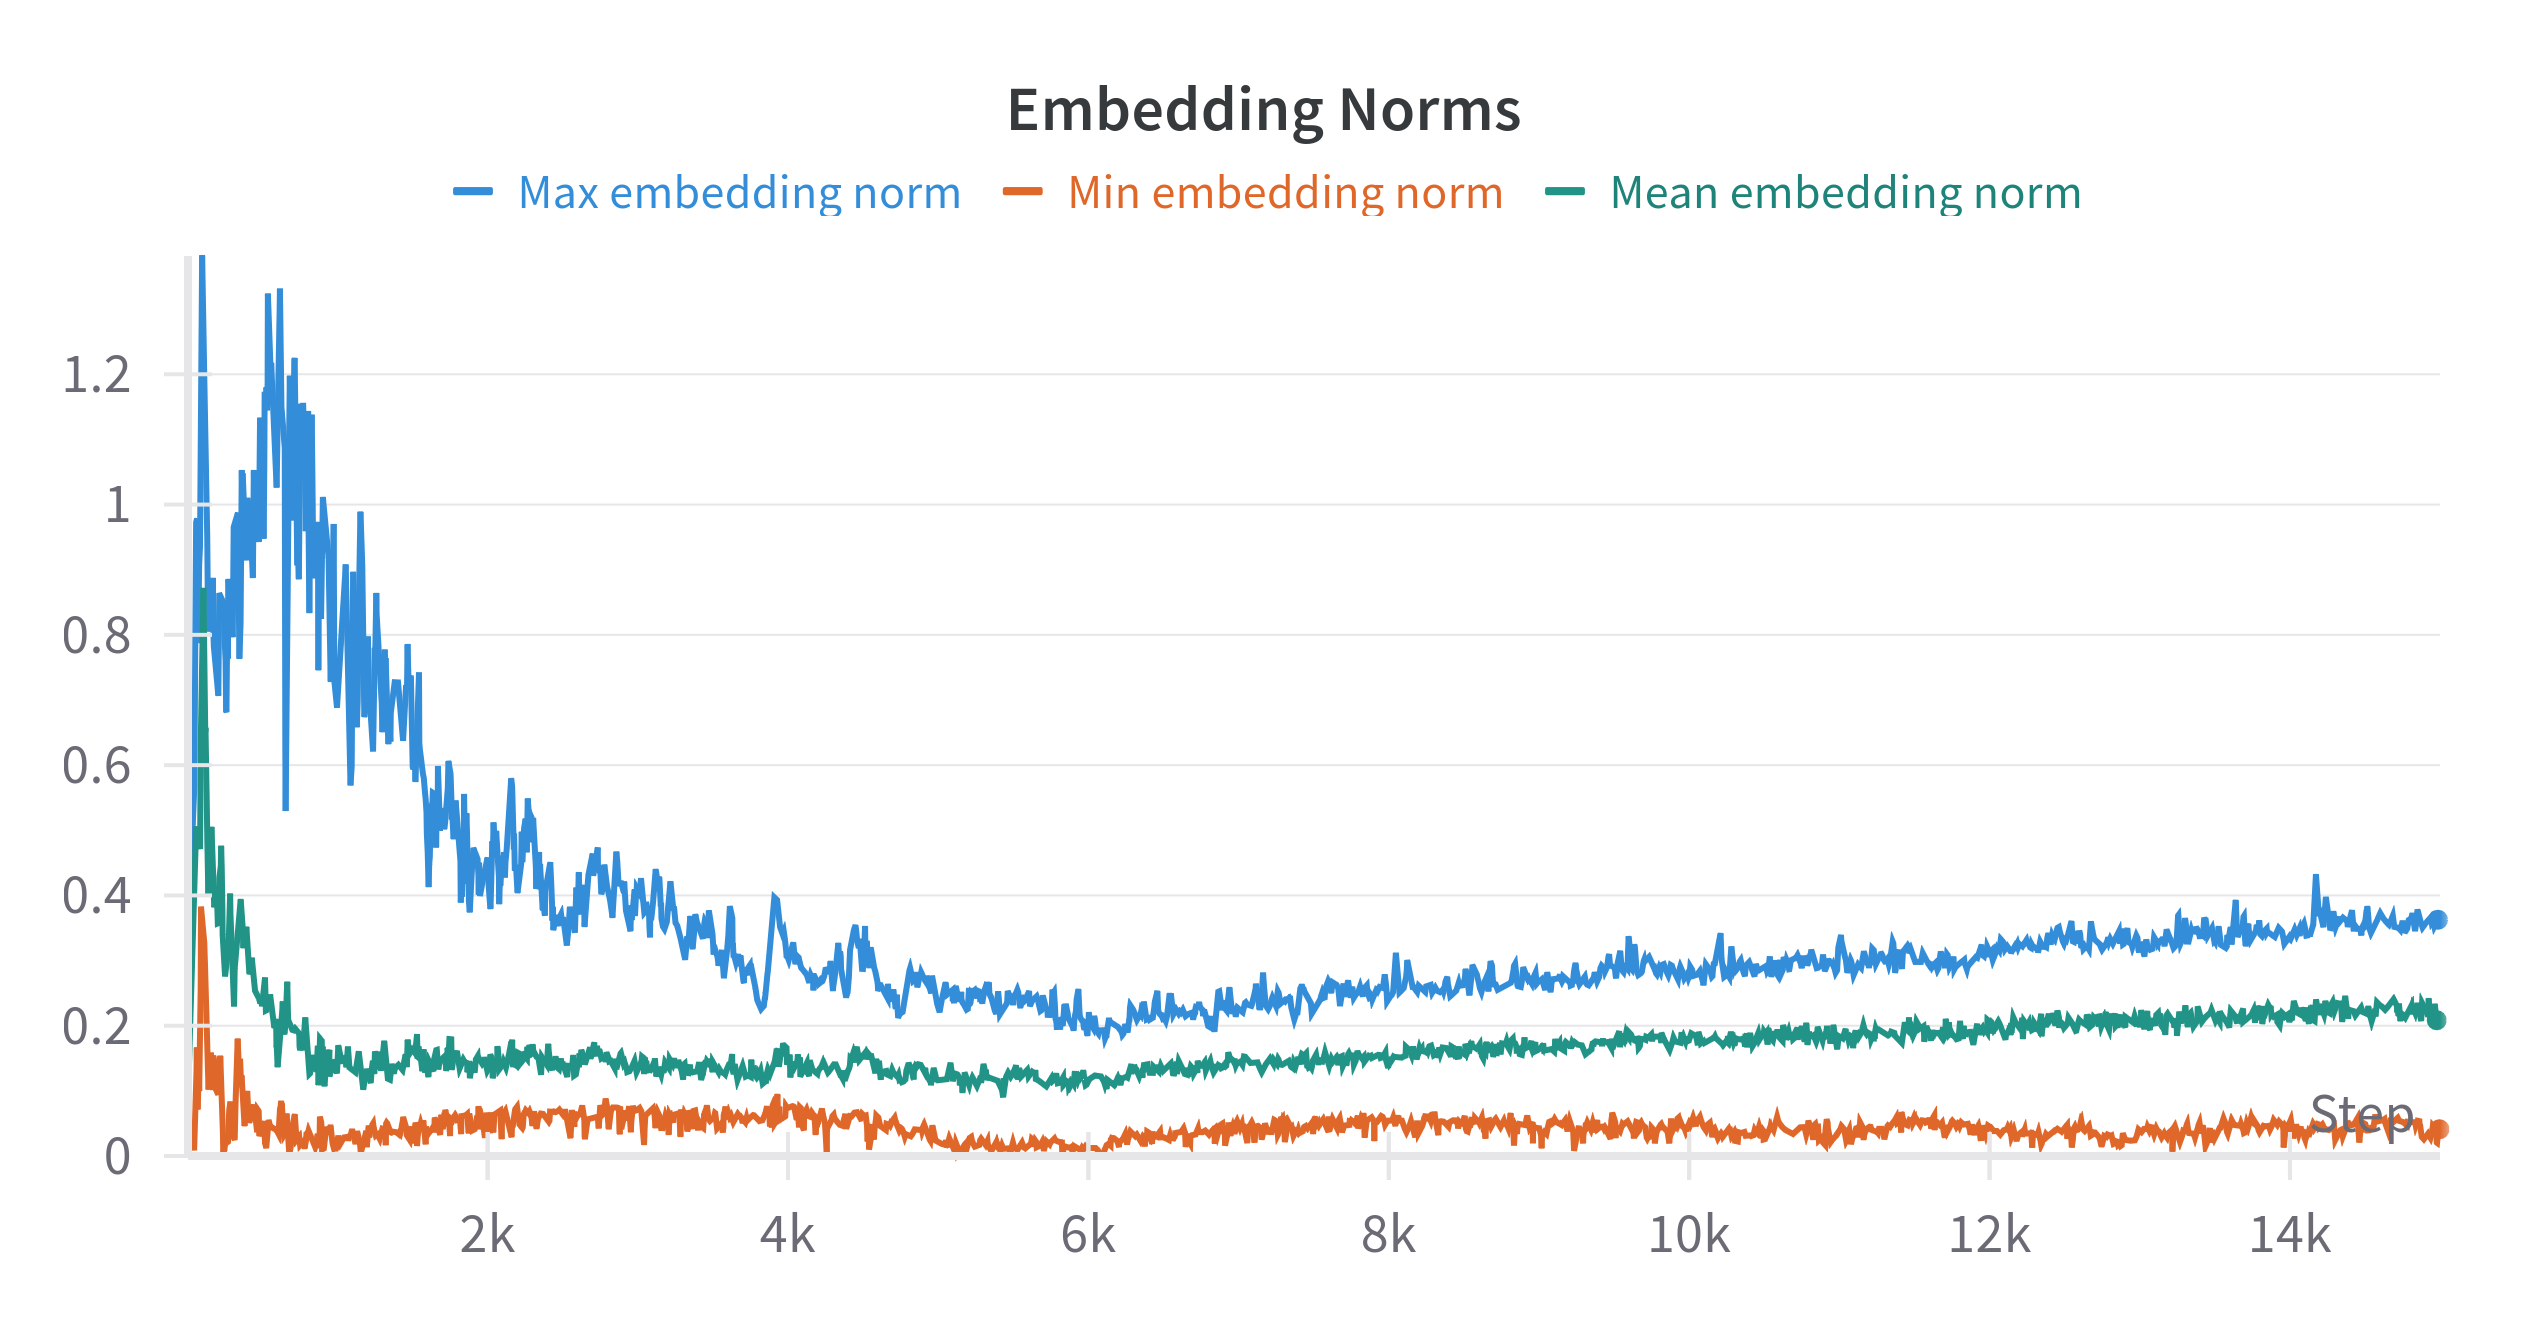
\includegraphics[width=0.8\linewidth]{informatica/wandb/mnist_corregido/batch_hard_embedding_norm.png}
        \caption{Normas de los \textit{embeddings}.}
    \end{subfigure}%
    \begin{subfigure}{.5\textwidth}
        \centering
        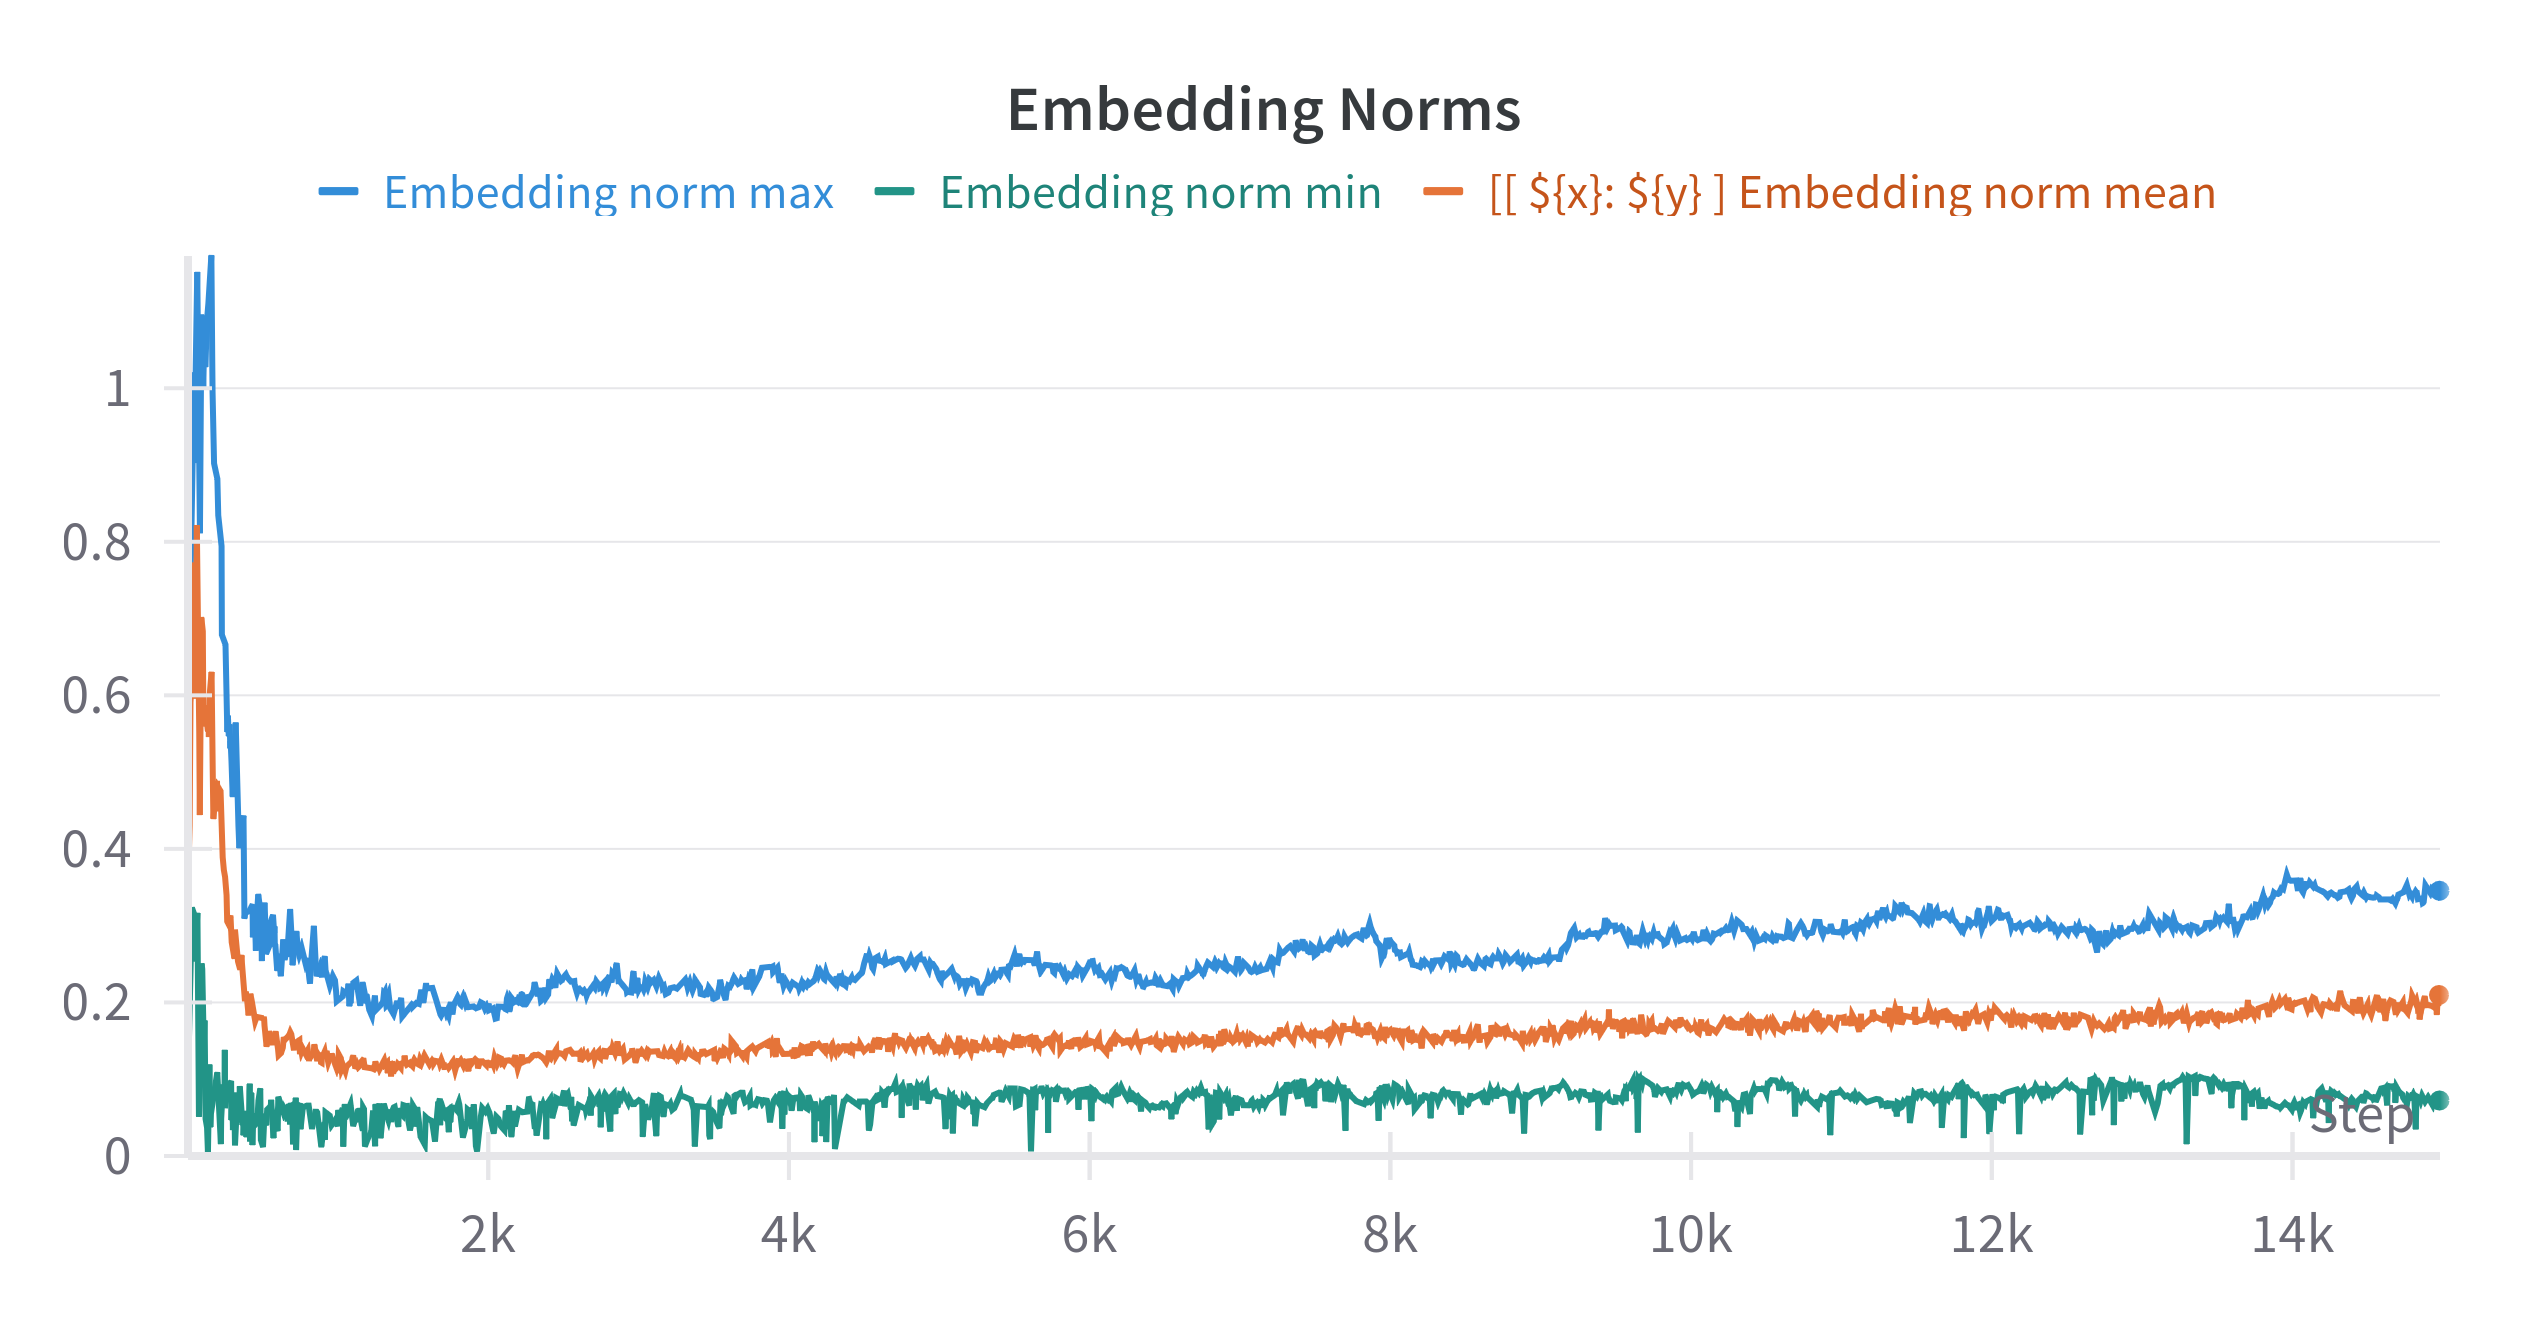
\includegraphics[width=0.8\linewidth]{informatica/wandb/mnist_corregido/batch_all_embedding_norm.png}
        \caption{Norma de los \textit{embeddings}.}
    \end{subfigure}

    \begin{subfigure}{.5\textwidth}
        \centering
        \includegraphics[width=0.8\linewidth]{informatica/wandb/mnist_corregido/batch_hard_intracluster.png}
        \caption{Distancias intracluster.}
    \end{subfigure}%
    \begin{subfigure}{.5\textwidth}
        \centering
        \includegraphics[width=0.8\linewidth]{informatica/wandb/mnist_corregido/batch_all_intracluster.png}
        \caption{Distancias intracluster.}
    \end{subfigure}

    \begin{subfigure}{.5\textwidth}
        \centering
        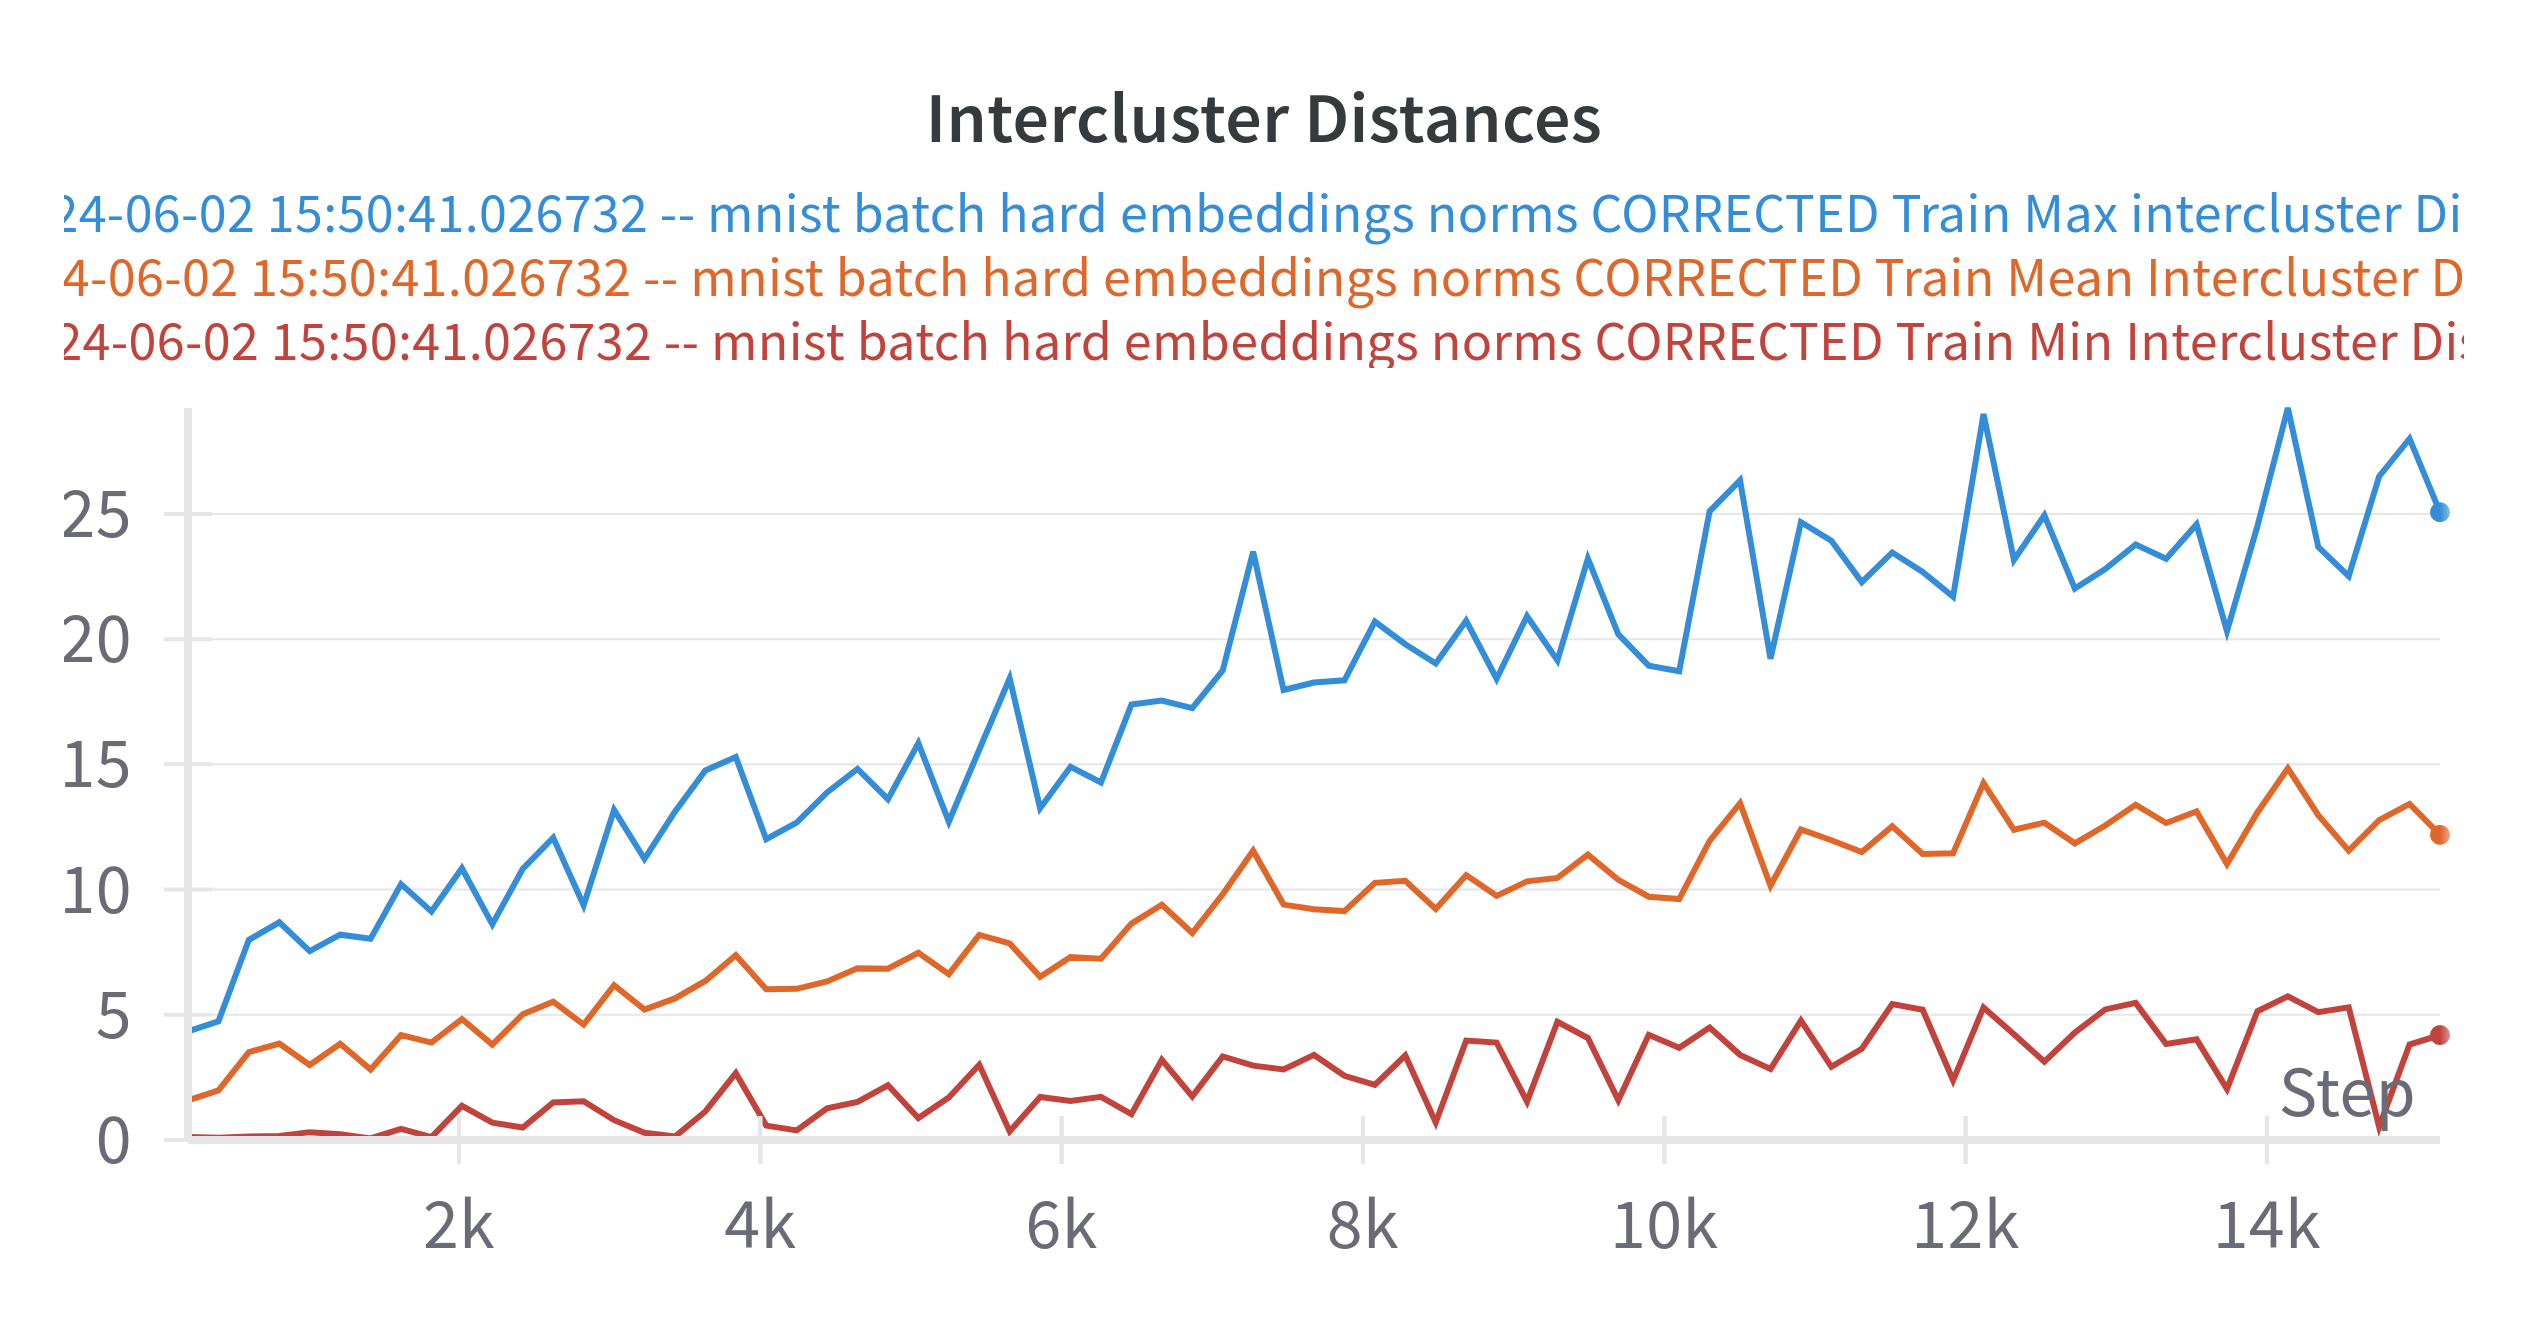
\includegraphics[width=0.8\linewidth]{informatica/wandb/mnist_corregido/batch_hard_interclusater.png}
        \caption{Distancias intercluster.}
    \end{subfigure}%
    \begin{subfigure}{.5\textwidth}
        \centering
        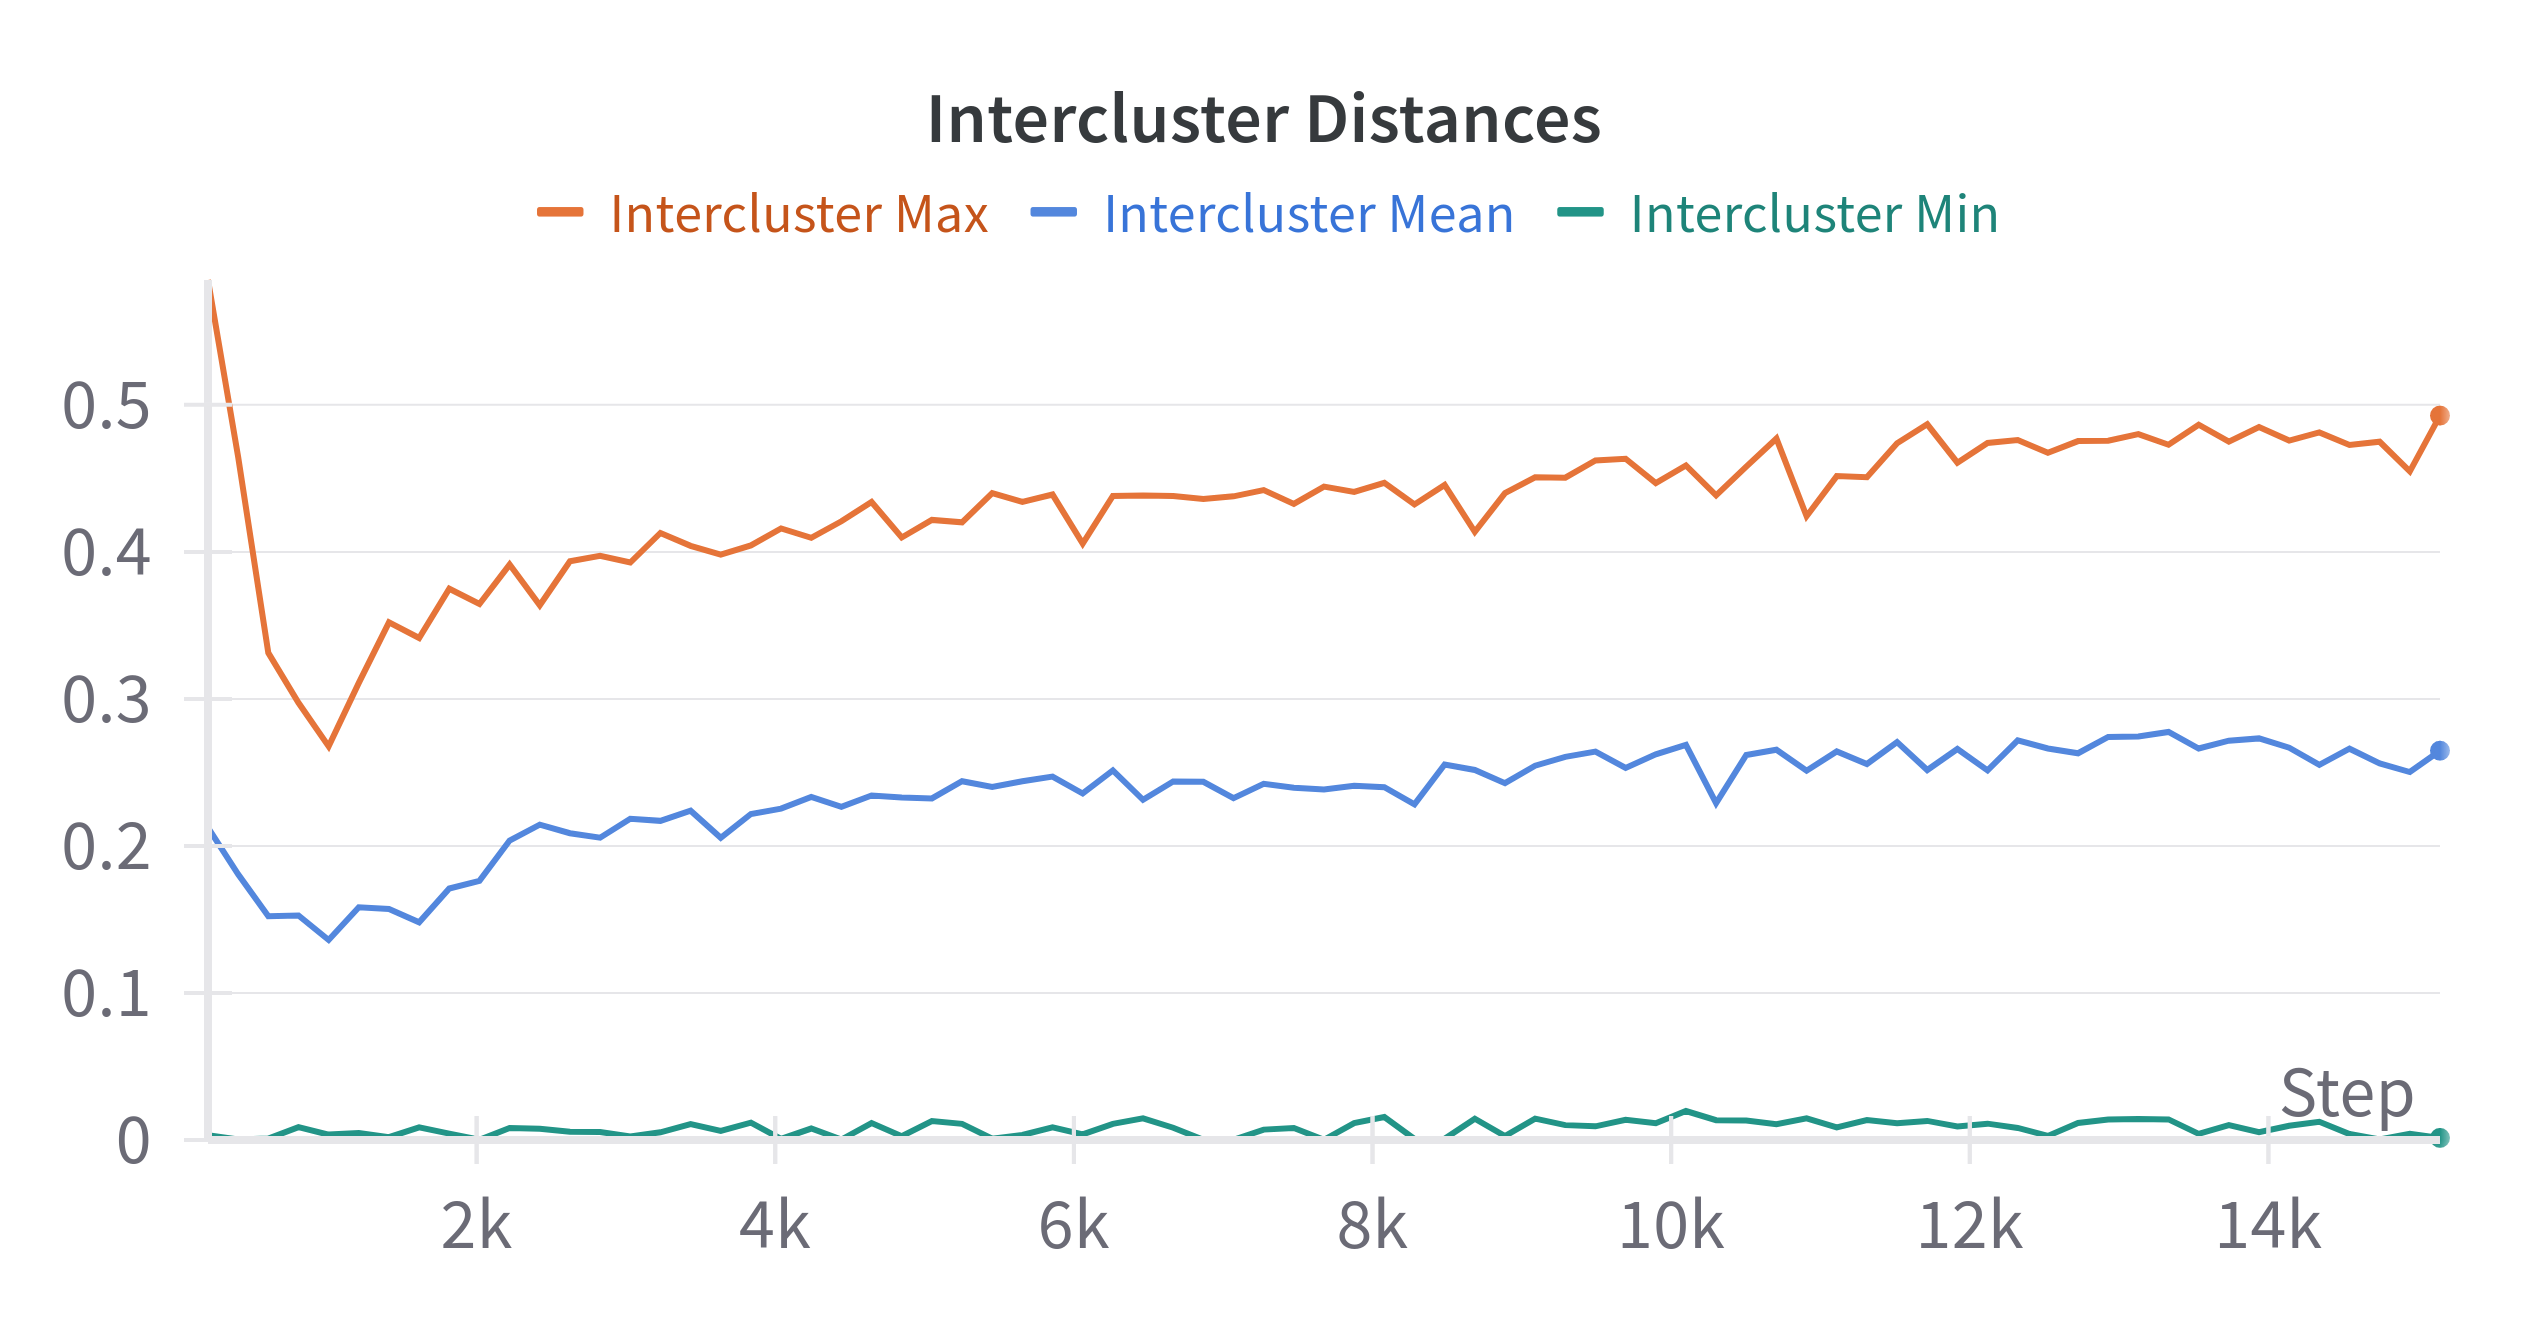
\includegraphics[width=0.8\linewidth]{informatica/wandb/mnist_corregido/batch_all_interclusater.png}
        \caption{Distancias intercluster}
    \end{subfigure}

    \caption{Distintas métricas observadas durante el proceso de entrenamiento. \textit{Batch Hard} se corresponde con las métricas de la izquierda, \textit{Batch All} con las métricas de la derecha.}
    \label{img:procesos_entrenamiento_mnist_corregido}
\end{figure}

\begin{figure}[!hbtp]
\centering
    \begin{subfigure}{.5\textwidth}
        \centering
        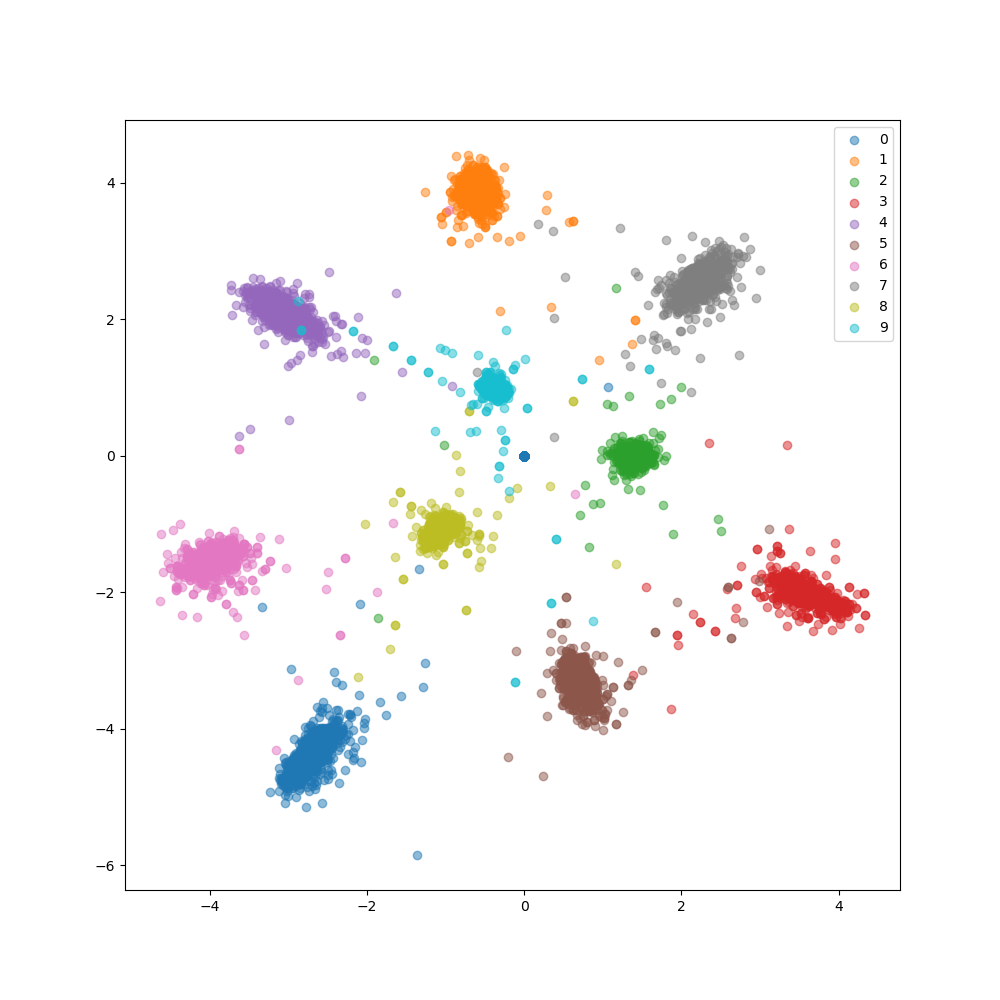
\includegraphics[width=0.8\linewidth]{informatica/wandb/mnist_corregido/batch_hard_2dplot_test.png}
        \caption{\textit{Batch Hard}}
    \end{subfigure}%
    \begin{subfigure}{.5\textwidth}
        \centering
        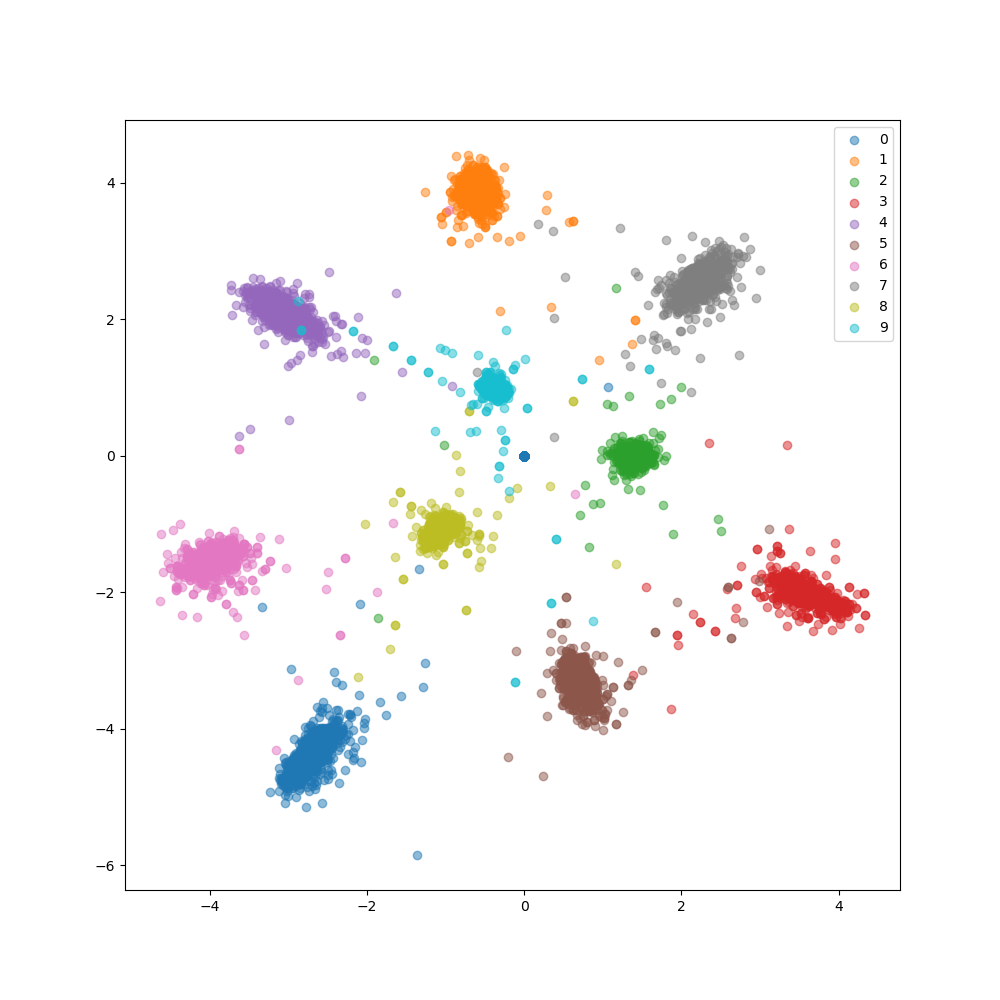
\includegraphics[width=0.8\linewidth]{informatica/wandb/mnist_corregido/batch_all_2dplot_test.png}
        \caption{\textit{Batch All}}
    \end{subfigure}
\caption{\textit{Embeddings} producidos sobre el conjunto de \textit{test}.}
\label{img:mnist_corregido_embeddings_aprendidos}
\end{figure}

\begin{table}[!hbtp]
    \centering
    \begin{tabular}{|l|l|l|l|}
        \hline
        Función de pérdida empleada & Métrica &  Conjunto & Valor \\
        \hline

        \textit{Batch Hard} & \textit{Rank@1 Accuracy} & Entrenamiento & 0.997 \\
        \textit{Batch Hard} & \textit{Rank@1 Accuracy} & Test & 0.992  \\
        \textit{Batch Hard} & \textit{Rank@5 Accuracy} & Entrenamiento & 0.997  \\
        \textit{Batch Hard} & \textit{Rank@5 Accuracy} & Test & 0.991 \\
        \textit{Batch Hard} & \textit{Silhouette} & Entrenamiento & 0.953 \\
        \textit{Batch Hard} & \textit{Silhouette} & Test & 0.922 \\
        \hline
        \textit{Batch All} & \textit{Rank@1 Accuracy} & Entrenamiento & 0.994 \\
        \textit{Batch All} & \textit{Rank@1 Accuracy} & Test & 0.992  \\
        \textit{Batch All} & \textit{Rank@5 Accuracy} & Entrenamiento & 0.994  \\
        \textit{Batch All} & \textit{Rank@5 Accuracy} & Test & 0.969 \\
        \textit{Batch All} & \textit{Silhouette} & Entrenamiento & 0.968 \\
        \textit{Batch All} & \textit{Silhouette} & Test & 0.949 \\


        \hline

    \end{tabular}
    \caption{Métricas de evaluación obtenidas sobre \textit{MNIST}, tras entrenar con la corrección aplicada a \textit{Batch Hard} y \textit{Batch All}.}
    \label{table:resultados_mnist_corregido}
\end{table}

\begin{table}[!hbtp]
    \centering
    \begin{tabular}{|l|l|l|l|l|}
        \hline
        Métrica & Conjunto & Antes & Después & Mejora \\
        \hline
        \textit{Rank@1 Accuracy} & Entrenamiento & 0.0937 & 0.997 & 10.64  \\
        \textit{Rank@1 Accuracy} & Test & 0.085 & 0.992 & 11.67  \\
        \textit{Rank@5 Accuracy} & Entrenamiento & 0.453 & 0.997 & 2.20 \\
        \textit{Rank@5 Accuracy} & Test & 0.414 & 0.991 & 2.39 \\
        \textit{Silhouette} & Entrenamiento & 0.000 & 0.953 & $\infty$ \\
        \textit{Silhouette} & Test & 0.000 & 0.922 & $\infty$ \\
        \hline

    \end{tabular}
    \caption{Comparación de los resultados obtenidos antes y después de aplicar nuestra solución. Los resultados tras aplicar la solución se muestran solo para \textit{Batch Hard}, ya que para el experimento inicial solo mostramos estos.}
    \label{table:comparaciones_mnist_resultados}
\end{table}

Observando la \imgref{img:procesos_entrenamiento_mnist_corregido} lo primero que destacamos es que en ambos casos las funciones de pérdida no se quedan estancadas en el valor del margen. En el caso de \textit{Batch Hard}, la función de pérdida tiende a cero y, en el caso de \textit{Batch All}, pasamos rápidamente a estar por debajo del margen $\alpha = 1.0$. Las normas de los \textit{embeddings} muestran un buen comportamiento, descienden rápidamente hasta estabilizarse y van aumentando ligeramente con el paso de las épocas de entrenamiento. Las distancias intracluster tienden a cero en \textit{Batch All} y se mantienen constantes en \textit{Batch Hard}. En ambos casos, las distancias intercluster crecen ligeramente con el paso de las épocas. Todo esto indica que la solución ha sido efectiva para ambas técnicas. Los resultados que muestran la \tableref{table:resultados_mnist_corregido} son muy contundentes en ambos casos. Tanto las métricas \textit{Rank@k accuracy} como los valores de \textit{Silhouette} son casi perfectos, tanto en entrenamiento como en \textit{test}, que es lo que cabe esperar en este conjunto de datos tan sencillo. Por lo tanto, \textbf{es claro que nuestra solución ha sido efectiva} a la hora de solucionar los problemas que estábamos teniendo. La \tableref{table:comparaciones_mnist_resultados} refuerza aún más esta conclusión. En las métricas originales \textit{Rank@k} estamos obteniendo resultados diez veces mejores. En las variantes locales, por la permisividad de estas, las mejoras bajan hasta algo más del doble. Y no podemos calcular mejoras sobre \textit{Silhouette} por ser nulas, pero cabe destacar que estamos pasando de uno de los peores valores de la métrica a un valor casi perfecto. Y los \textit{embeddings} producidos sobre los conjuntos de \textit{test} que mostramos en la \imgref{img:mnist_corregido_embeddings_aprendidos} muestran visualmente que el modelo está aprendiendo adecuadamente a resolver el problema planteado.

\subsection{Resultados sobre \textit{CACD} con nuestra propuesta de solución} \label{isubsec:experimentacion_cacd_bien}

Repetimos el mismo procedimiento que en el experimento anterior. Realizamos dos experimentos, uno con \textit{Batch Hard} y otro con \textit{Batch All}, tras implementar nuestra propuesta de solución. En este punto nuestro objetivo es lograr una mejora de rendimiento considerable que valide la efectividad de nuestra solución. Sin embargo, por la complejidad del problema, no esperamos obtener resultados competitivos con el estado del arte, ni siquiera resultados que permitan utilizar esta red en una aplicación real. Por lo tanto, usaremos únicamente \textit{CACD}, tanto para entrenar como para validar. Para ello, reservamos un 20\% del conjunto de datos para el \textit{holdout}. Además, lo hacemos de forma disjunta, es decir, en el conjunto de test no existen identidades que hayamos visto durante el entrenamiento.

Los hiperparámetros empleados para los dos experimentos se recogen en la tabla \tableref{table:hp_cacd_corregido}. Esta vez hemos realizado algunos cambios en estos valores. Como hemos comentado, nuestro objetivo ahora no es conseguir los mejores resultados sino validar que la solución es efectiva. Esto, junto con la falta de tiempo para lanzar un proceso de búsqueda de hiperparámetros, hace que escojamos estos valores en base a nuestra experiencia y tras haber realizado una exploración manual con pequeños experimentos. El proceso de entrenamiento puede estudiarse en la \imgref{img:proceso_entrenamiento_cacd_corregido} y los resultados producidos se exponen en la \tableref{table:resultados_cacd_corregido}.

\begin{table}[!hbt]
    \centering
    \begin{tabular}{|l|l|}
        \hline
        Hiperparámetro                                    & Valor escogido        \\
        \hline
        P                                                 & 16                    \\
        K                                                 & 4                     \\
        Arquitectura de la red                            & \textit{CACDResNet18} \\
        Uso de normalización                              & No                    \\
        Dimensión del \textit{embedding}                  & 10                    \\
        \textit{Learning Rate}                            & 0.0001                \\
        Uso de \textit{Softplus}                          & No                    \\
        Penalización en la norma de las salidas           & No                    \\
        Factor de penalización en la norma de las salidas & -                     \\
        Uso de \textit{Gradient Clipping}                 & No                    \\
        Valor máximo del \textit{Gradient Clipping}       & -                     \\
        $\alpha$                                          & 1.0                   \\

        \hline
    \end{tabular}
    \caption{Hiperparámetros empleados en los dos experimentos, uno para \textit{Batch Hard} y otro para \textit{Batch All}.}
    \label{table:hp_cacd_corregido}
\end{table}

\begin{figure}[!hbtp]
    \centering
    \begin{subfigure}{.5\textwidth}
        \centering
        \includegraphics[width=0.8\linewidth]{informatica/wandb/cacd_corregido/batch_hard_running_loss.png}
        \caption{Función de pérdida.}
    \end{subfigure}%
    \begin{subfigure}{.5\textwidth}
        \centering
        \includegraphics[width=0.8\linewidth]{informatica/wandb/cacd_corregido/batch_hard_running_loss.png}
        \caption{Función de pérdida.}
    \end{subfigure}

    \begin{subfigure}{.5\textwidth}
        \centering
        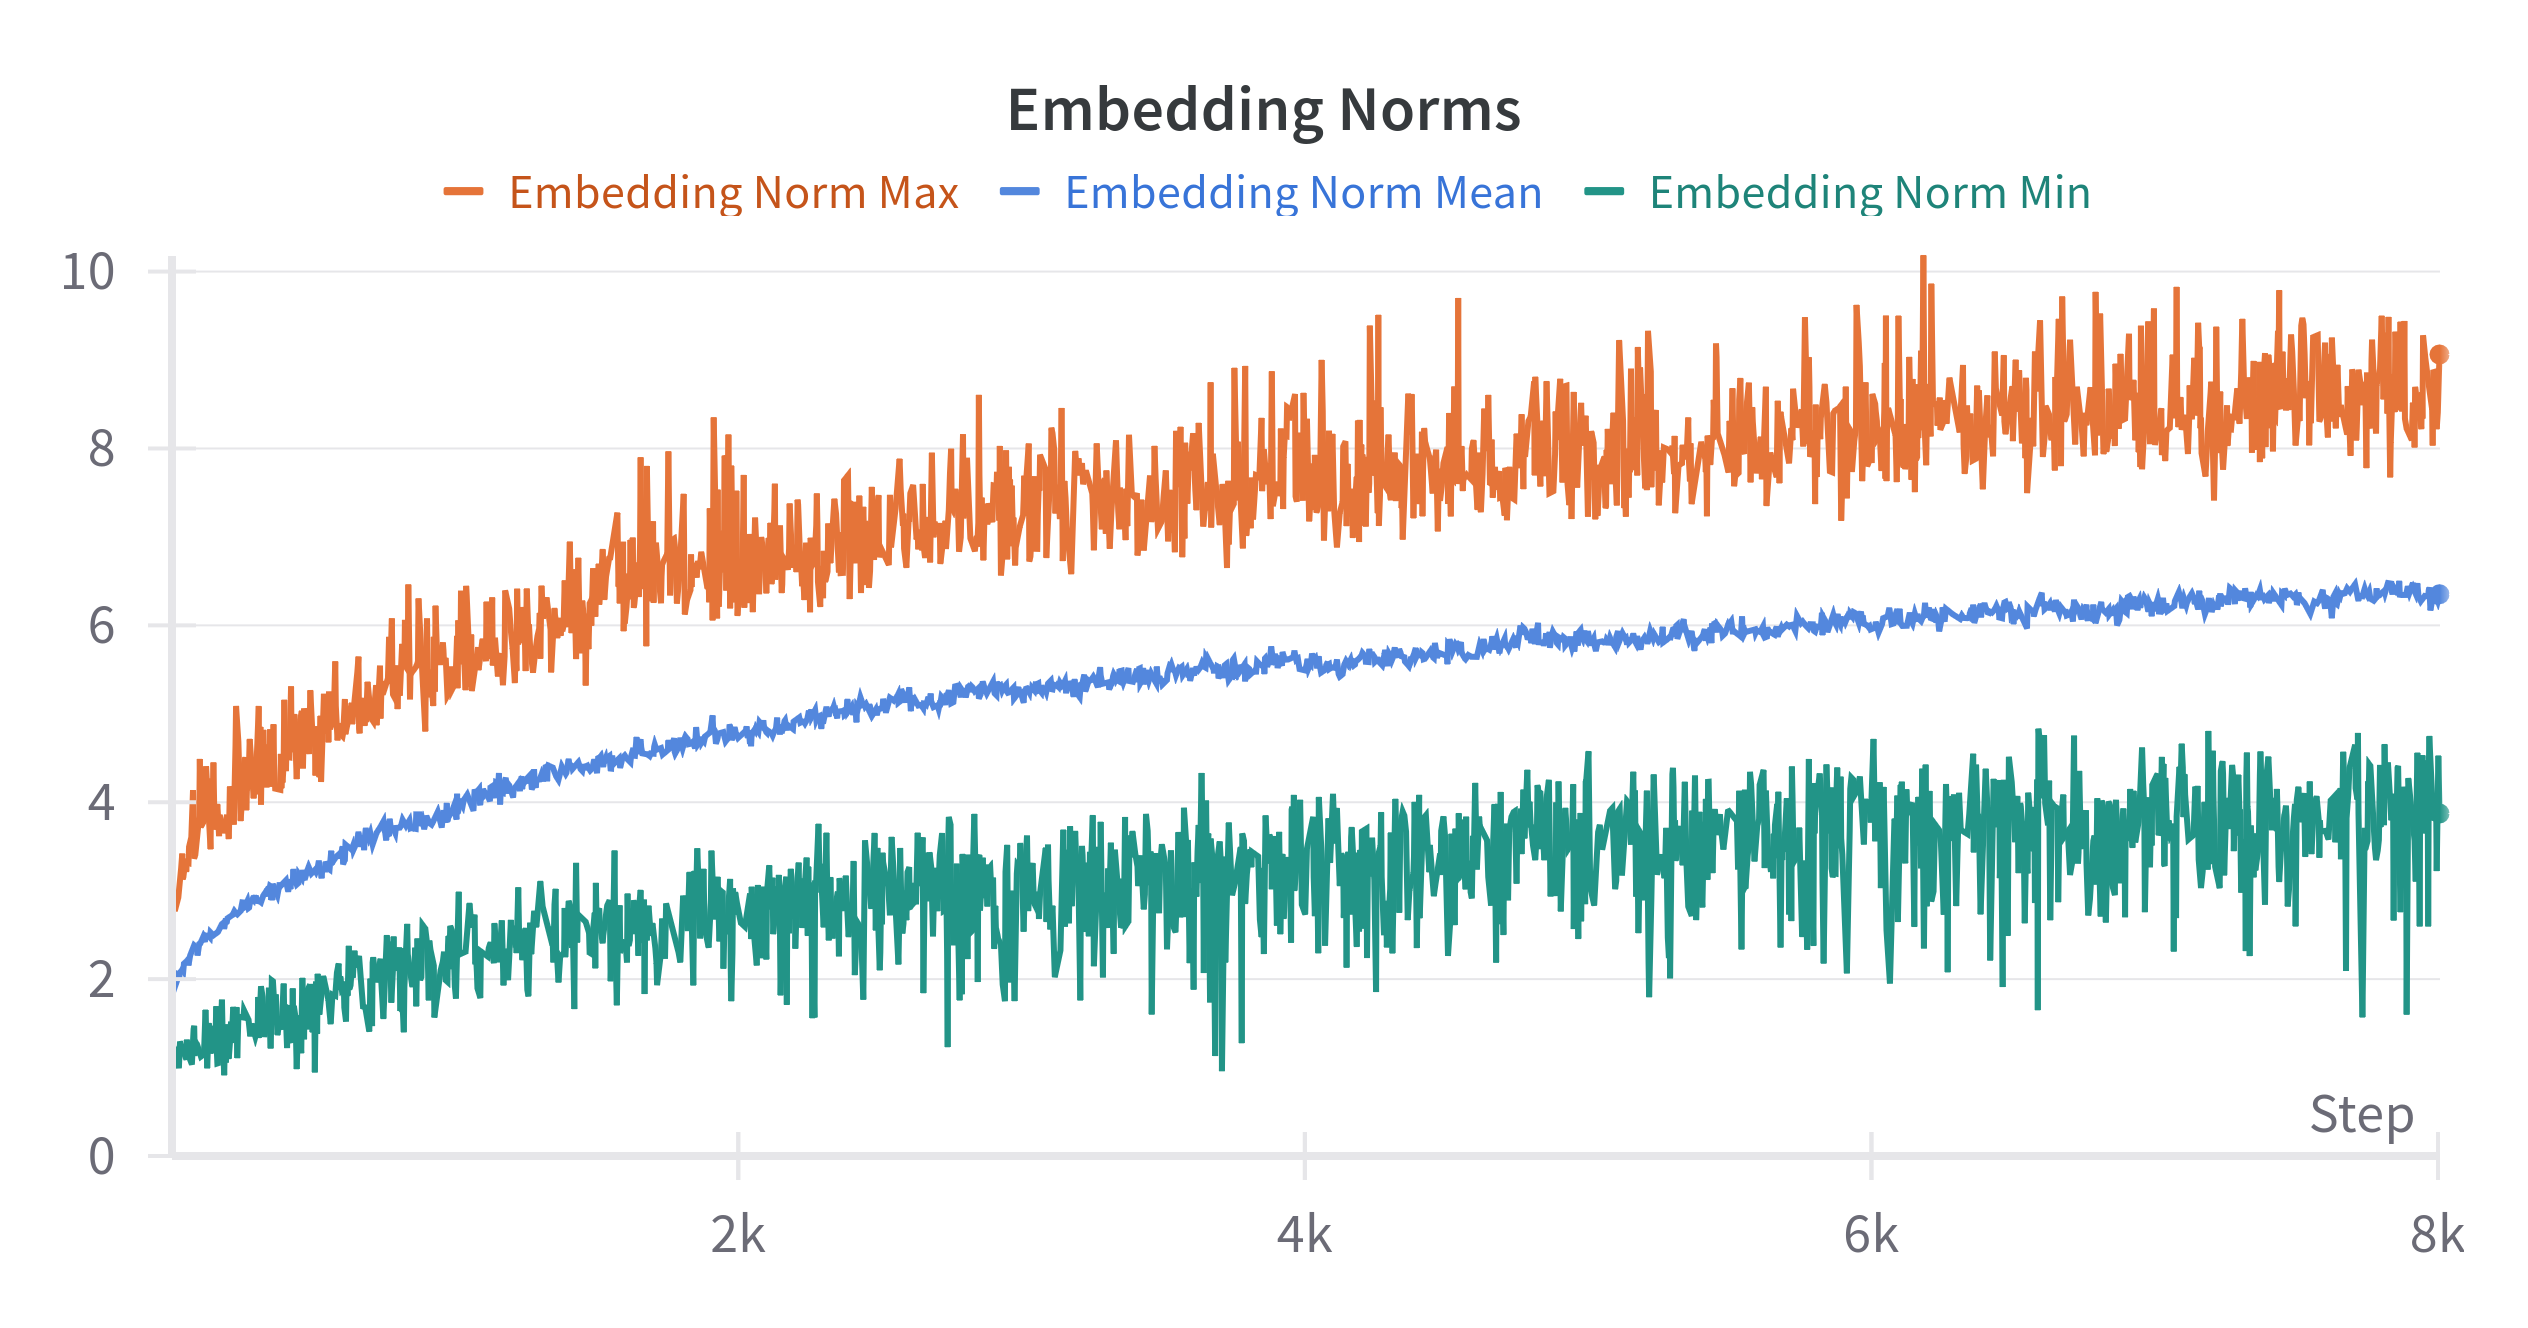
\includegraphics[width=0.8\linewidth]{informatica/wandb/cacd_corregido/batch_hard_embedding_norms.png}
        \caption{Norma de los \textit{embeddings}.}
    \end{subfigure}%
    \begin{subfigure}{.5\textwidth}
        \centering
        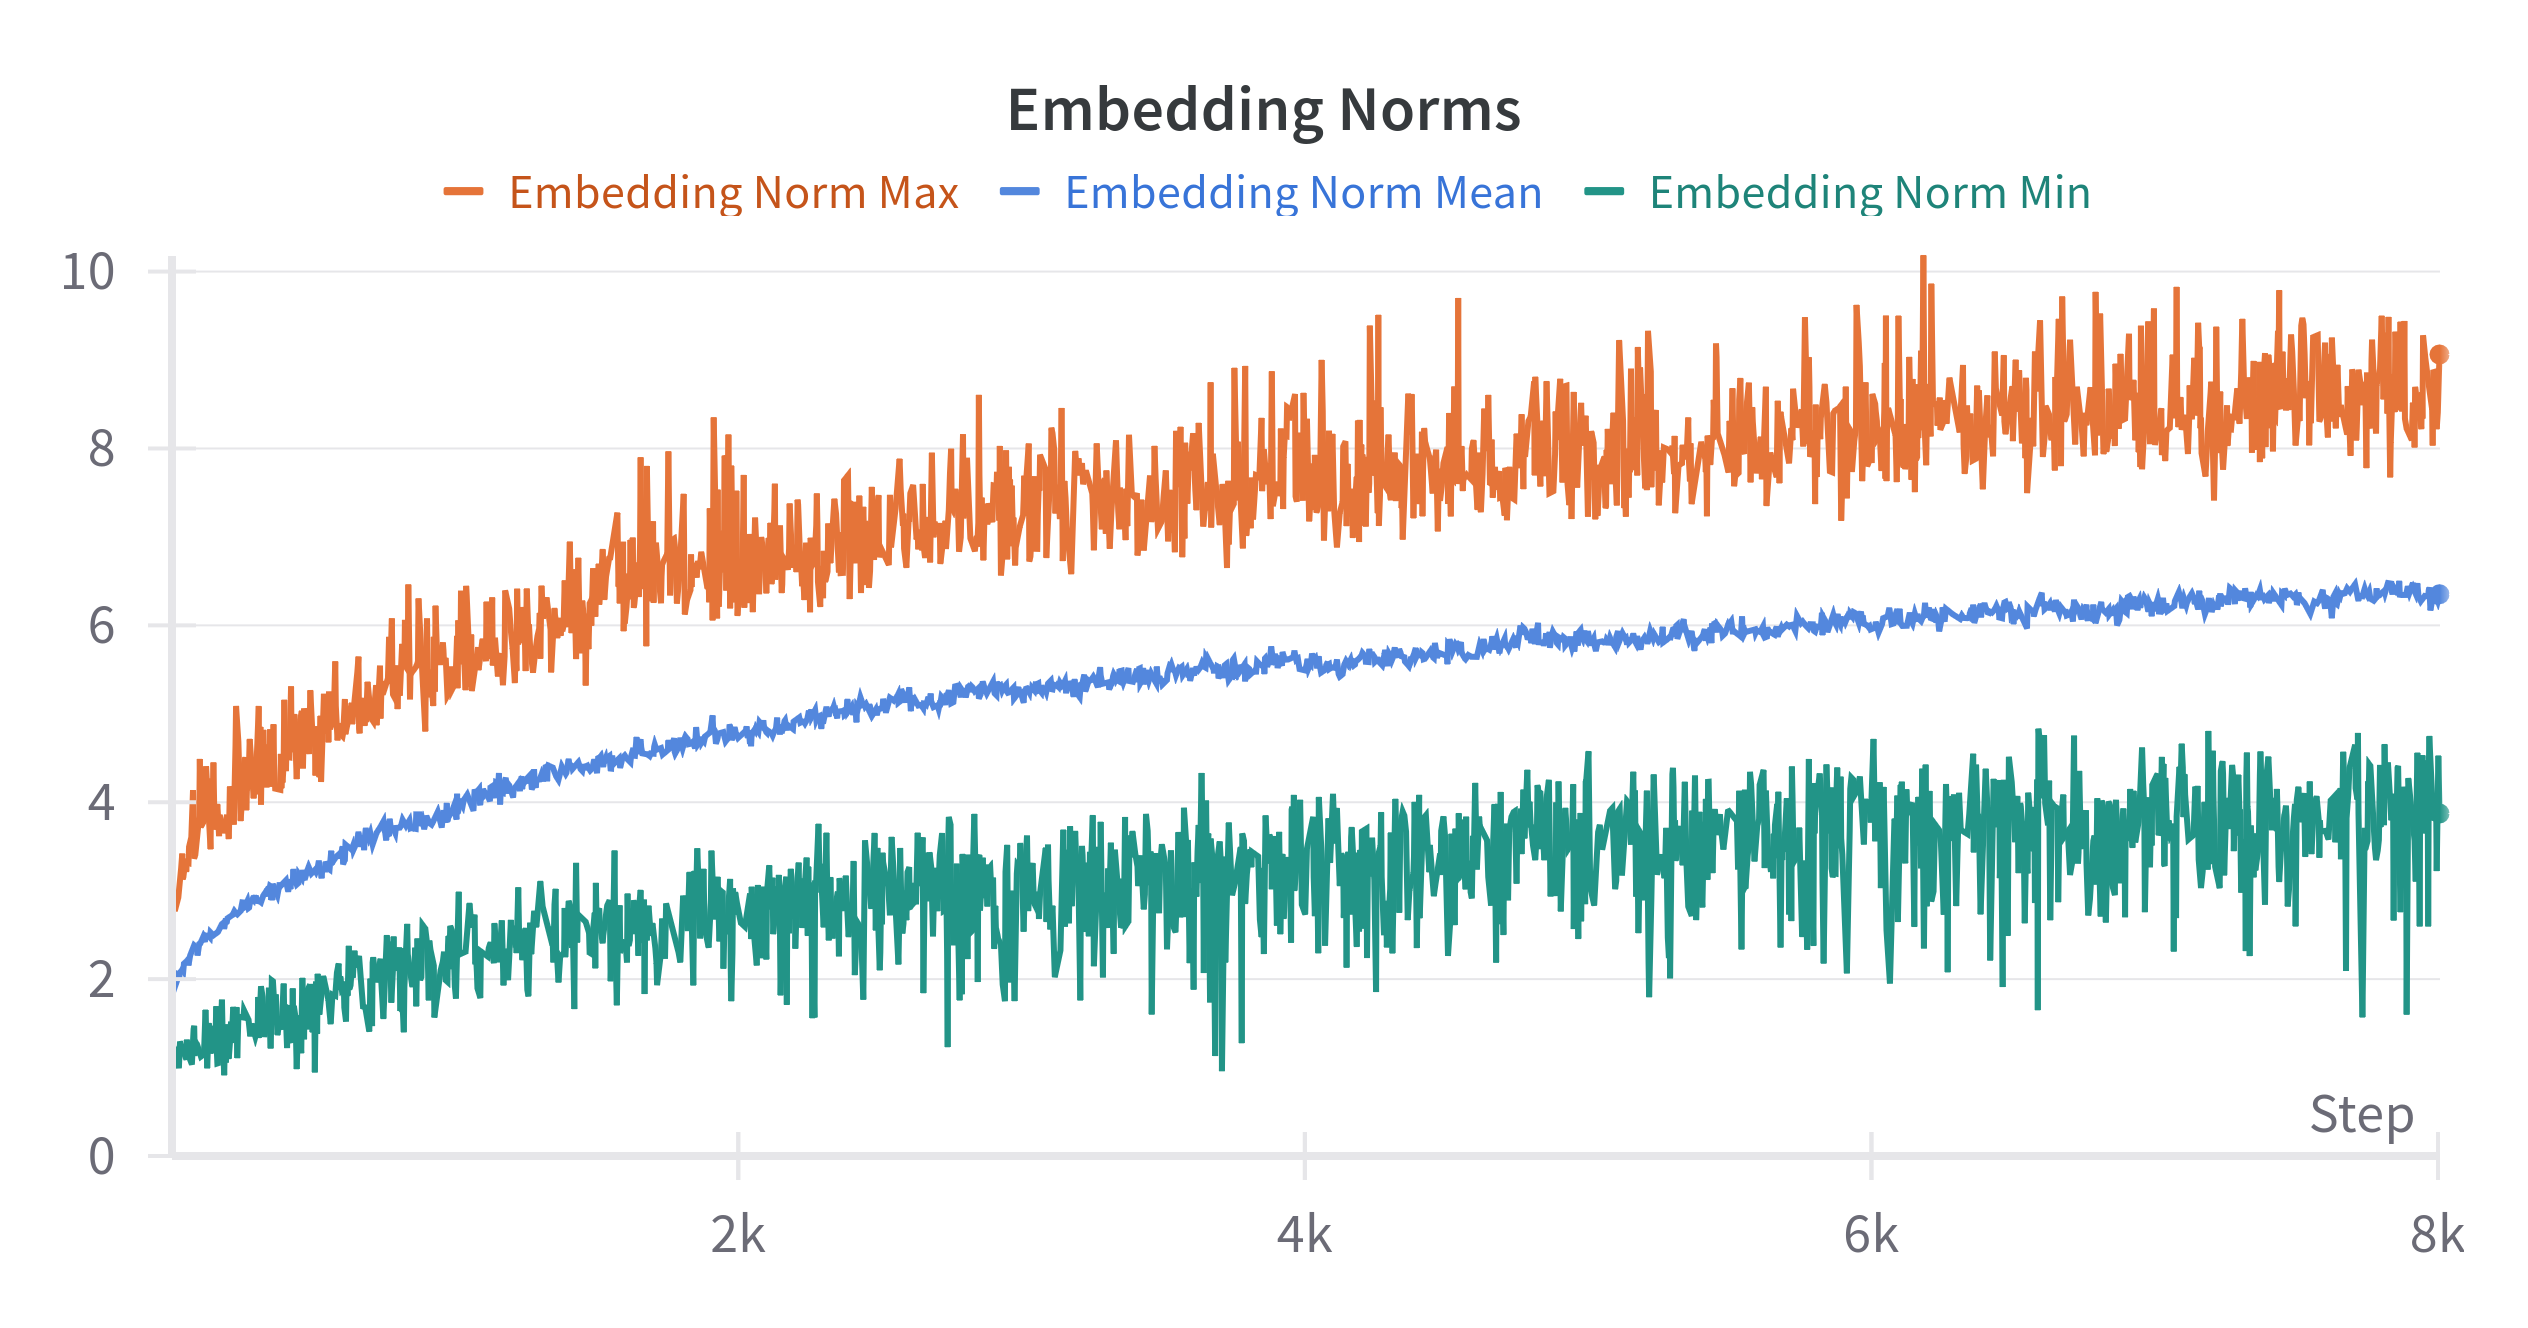
\includegraphics[width=0.8\linewidth]{informatica/wandb/cacd_corregido/batch_hard_embedding_norms.png}
        \caption{Norma de los \textit{embeddings}.}
    \end{subfigure}

    \begin{subfigure}{.5\textwidth}
        \centering
        \includegraphics[width=0.8\linewidth]{informatica/wandb/cacd_corregido/batch_hard_intracluster.png}
        \caption{Distancias intracluster.}
    \end{subfigure}%
    \begin{subfigure}{.5\textwidth}
        \centering
        \includegraphics[width=0.8\linewidth]{informatica/wandb/cacd_corregido/batch_all_intracluster.png}
        \caption{Distancias intracluster.}
    \end{subfigure}

    \begin{subfigure}{.5\textwidth}
        \centering
        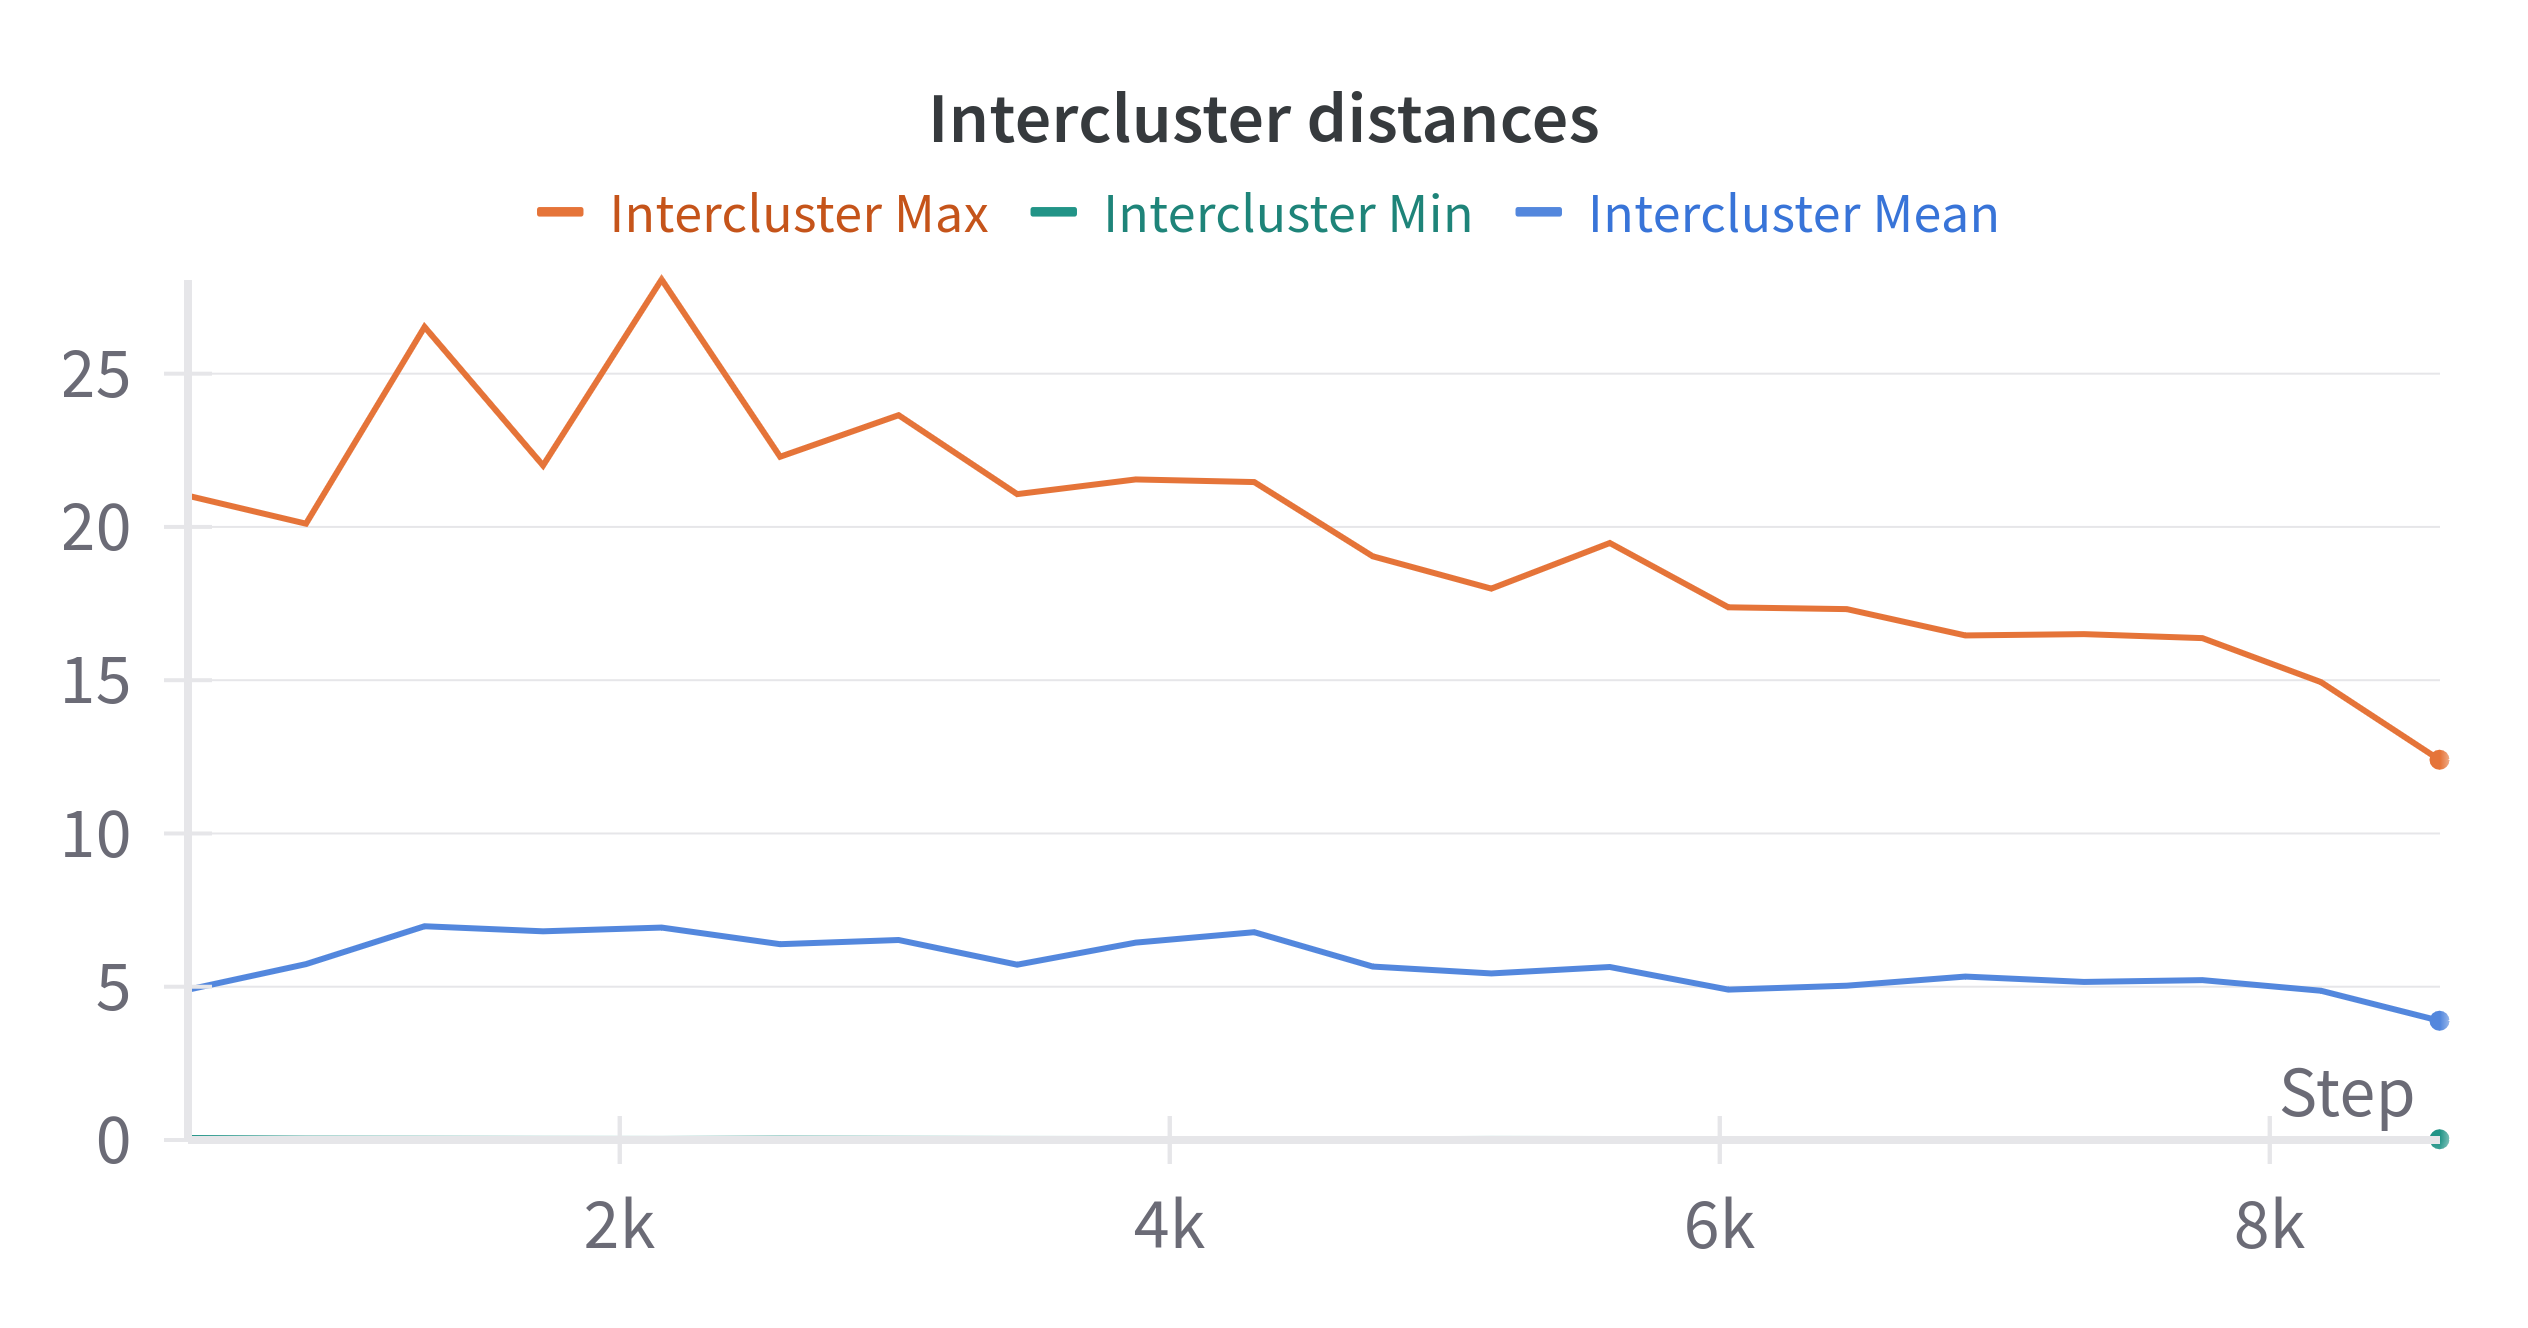
\includegraphics[width=0.8\linewidth]{informatica/wandb/cacd_corregido/batch_hard_intercluster.png}
        \caption{Distancias intercluster.}
    \end{subfigure}%
    \begin{subfigure}{.5\textwidth}
        \centering
        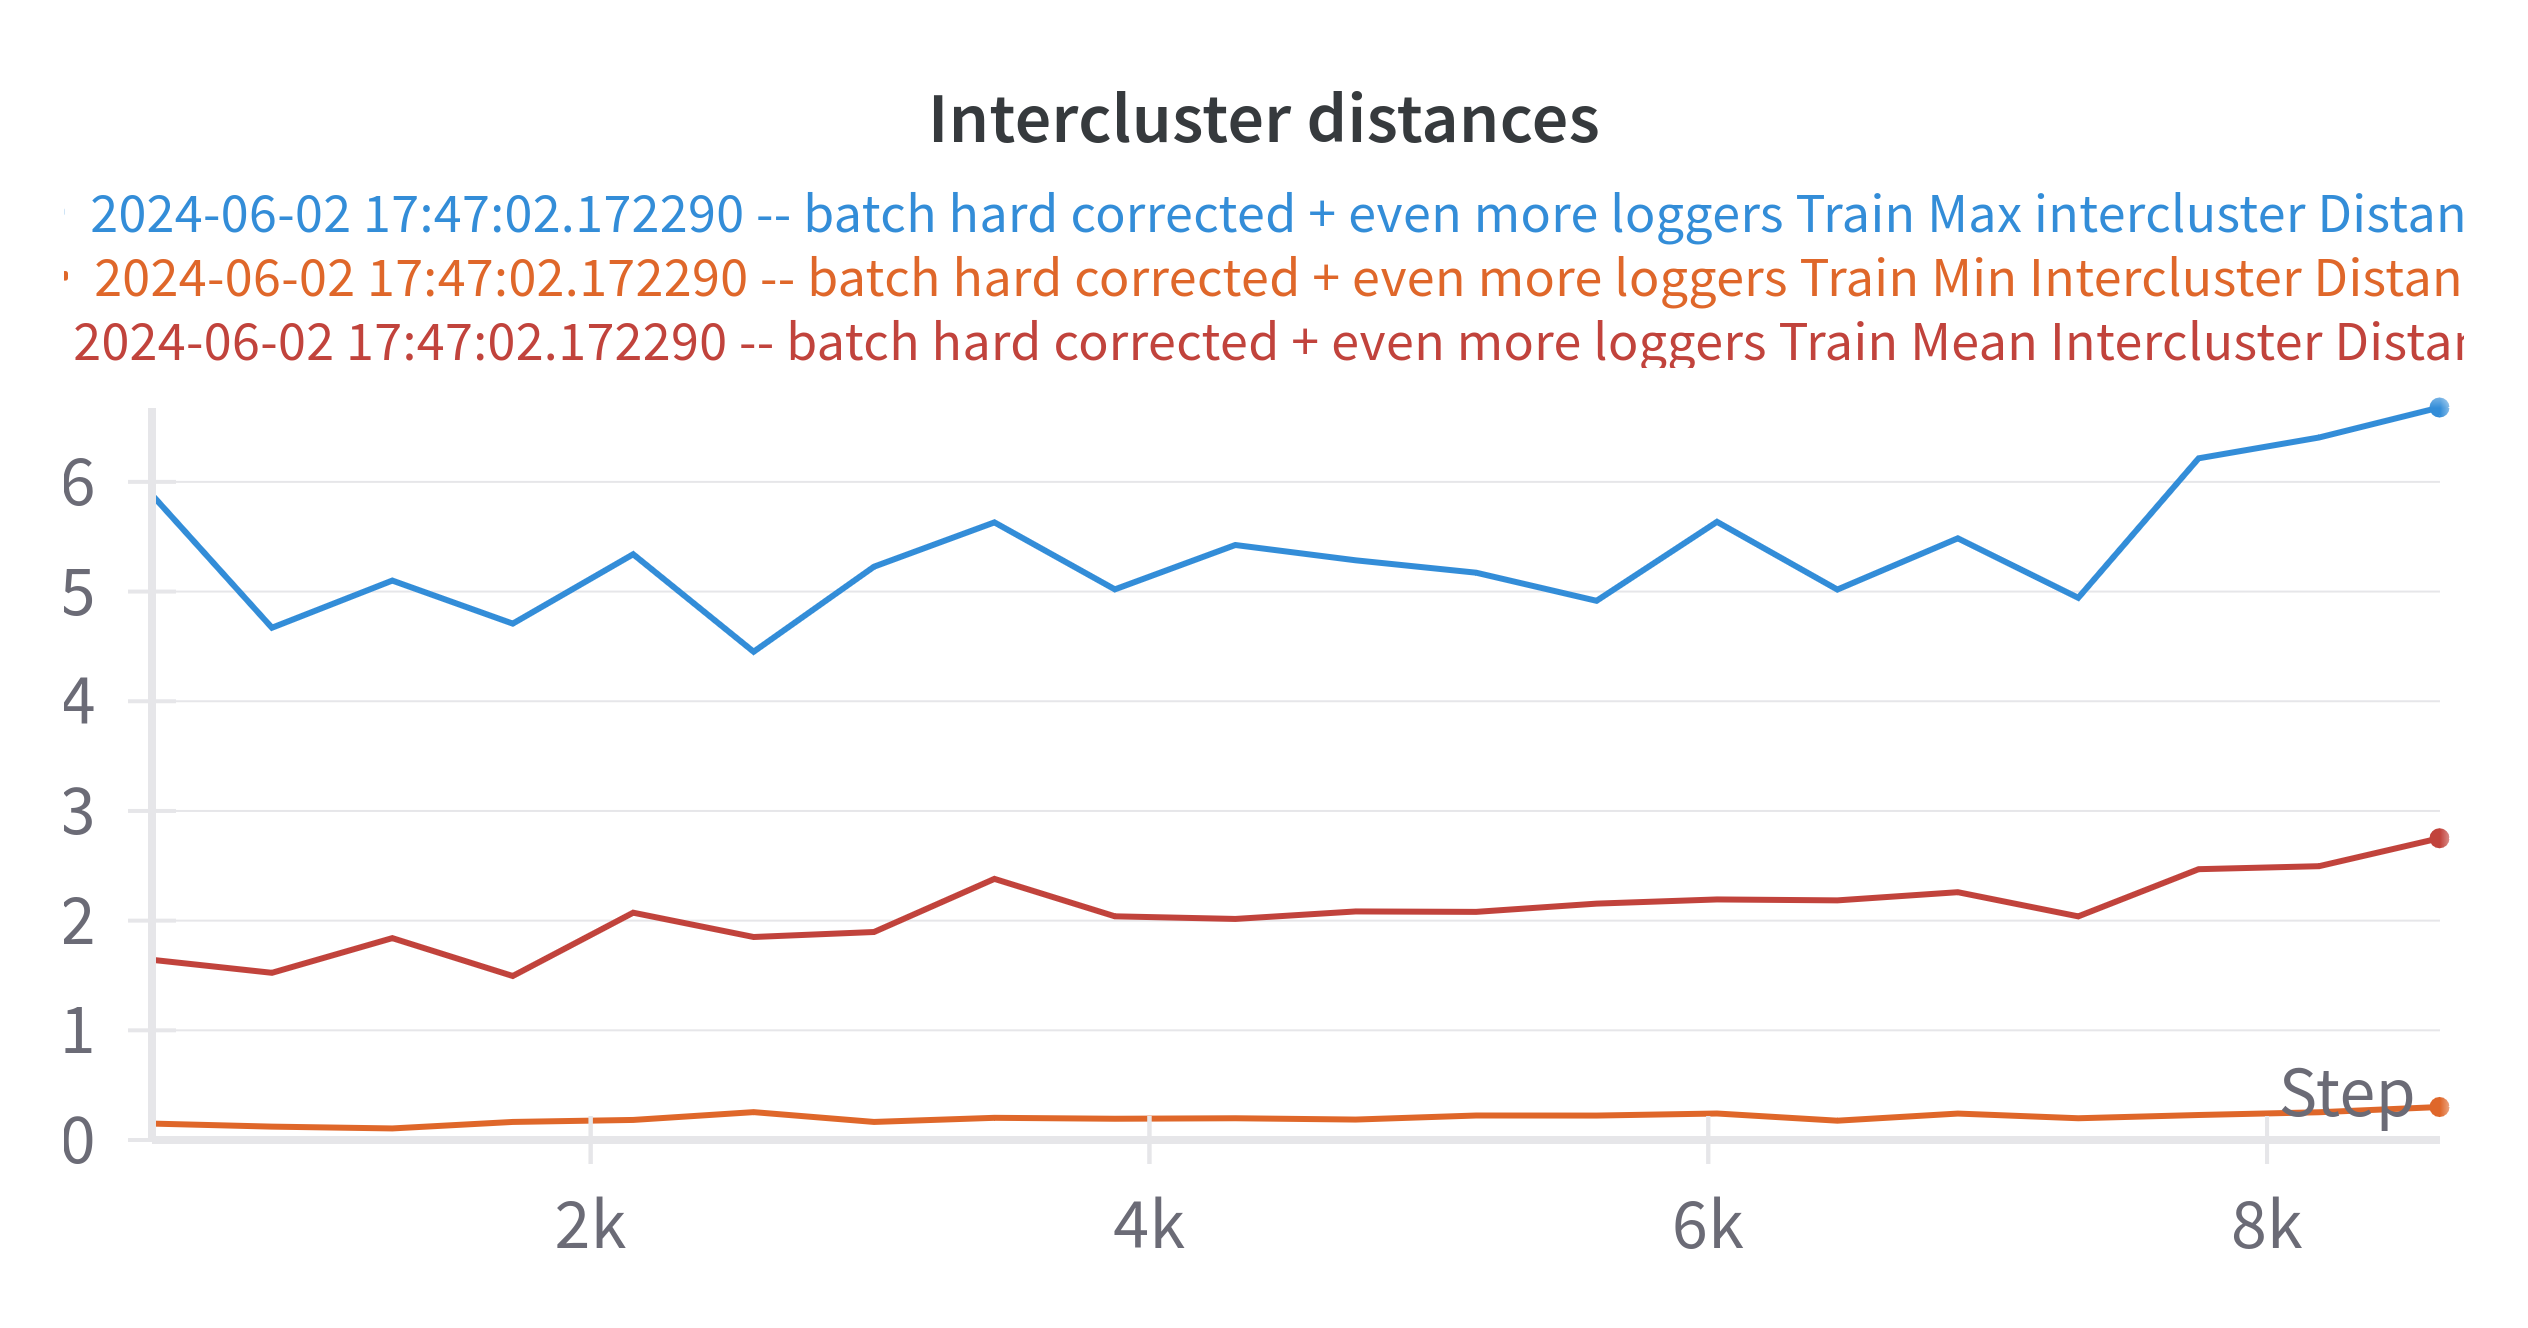
\includegraphics[width=0.8\linewidth]{informatica/wandb/cacd_corregido/batch_all_intercluster.png}
        \caption{Distancias intercluster.}
    \end{subfigure}
    \caption{Métricas observadas durante el proceso de entrenamiento. \textit{Batch Hard} se corresponde con las métricas de la izquierda, \textit{Batch All} con las métricas de la derecha.}
    \label{img:proceso_entrenamiento_cacd_corregido}
\end{figure}

\begin{table}[!hbtp]
\centering
\begin{tabular}{|l|l|l|l|}
    \hline
    Función de pérdida empleada & Métrica &  Conjunto & Valor \\
    \hline

    \textit{Batch Hard} & \textit{Rank@1 Accuracy} & Entrenamiento & 0.2676 \\
    \textit{Batch Hard} & \textit{Rank@1 Accuracy} & Test  & 0.3732  \\
    \textit{Batch Hard} & \textit{Rank@5 Accuracy} & Entrenamiento & 0.4639  \\
    \textit{Batch Hard} & \textit{Rank@5 Accuracy} & Test & 0.6152 \\
    \textit{Batch Hard} & \textit{Silhouette} & Entrenamiento & -0.1648 \\
    \textit{Batch Hard} & \textit{Silhouette} & Test & -0.1832 \\

    \hline

    \textit{Batch All} & \textit{Rank@1 Accuracy} & Entrenamiento & 0.1757 \\
    \textit{Batch All} & \textit{Rank@1 Accuracy} & Test & 0.3125  \\
    \textit{Batch All} & \textit{Rank@5 Accuracy} & Entrenamiento & 0.4126  \\
    \textit{Batch All} & \textit{Rank@5 Accuracy} & Test & 0.5816 \\
    \textit{Batch All} & \textit{Silhouette} & Entrenamiento & -0.1513 \\
    \textit{Batch All} & \textit{Silhouette} & Test & -0.1171 \\

    \hline

\end{tabular}
\caption{Métricas de evaluación obtenidas sobre \textit{CACD} y \textit{FG-Net}, tras entrenar con la corrección aplicada a \textit{Batch Hard} y \textit{Batch All}.}
\label{table:resultados_cacd_corregido}
\end{table}

Se repite la mejora de comportamiento observada en la anterior experimentación sobre \textit{MNIST}, aunque esta vez los resultados no sean tan buenos. En la \imgref{img:proceso_entrenamiento_cacd_corregido} podemos ver que las funciones de pérdida ya no se quedan atascadas en el valor del margen. Sin embargo, esta vez quedan por encima de dicho valor del margen disminuyendo lentamente. Esto nos indica que quizás deberíamos emplear otros hiperparámetros para lograr mejores resultados. Por ejemplo, tiempos de entrenamiento más largos o valores distintos para el \textit{learning rate}. Pero de nuevo, nuestro objetivo ahora no es obtener el mejor modelo posible sino validar la eficacia de nuestra solución. Las normas de los \textit{embeddings} muestran el comportamiento deseado, incrementan con el paso de las épocas de entrenamiento. Las distancias intracluster e intercluster ya no tienden a cero, aunque se mantienen estáticas y no parecen aumentar lo suficiente. Una vez más, esto es compatible con una solución eficaz, pero necesitaríamos realizar un estudio más profundo de otros factores para obtener buenos resultados. Por otro lado, los resultados expuestos en la \tableref{table:resultados_cacd_corregido} son buenos. Aunque estén alejados de ser realmente competentes, son más que suficientes para validar nuestra solución. Los valores de las métricas \textit{Rank@k} han mejorado significativamente en ambos casos. Los valores de \textit{Silhouette} siguen siendo igual de malos, otra vez, esto nos indica que para obtener un modelo con alto rendimiento deberíamos realizar un estudio en profundidad de la arquitectura e hiperparámetros utilizados. Cabe destacar que el rendimiento del modelo entrenado usando \textit{Batch All} es algo menor que el entrenado con \textit{Batch Hard}, pero sigue siendo suficiente para validar la eficacia de nuestra solución.

Para poder comparar adecuadamente respecto a la implementación sin corrección, repetiremos el experimento sin corrección usando los hiperparámetros especificados en la \tableref{table:hp_cacd_corregido}. Además, como ya hemos comentado previamente, usaremos una parte de \textit{CACD} para evaluar el modelo, en vez de usar \textit{FG-Net}. No volvemos a mostrar el proceso de entrenamiento pues los comportamientos que hemos estudiado no cambian con estos nuevos hiperparámetros. Así que únicamente mostramos los resultados en la \tableref{table:resultados_cacd_mal_nueva} y la comparación entre experimentos antes y después de la corrección en la \tableref{table:comparaciones_cacd_resultados}.


\begin{table}[!hbtp]
\centering
\begin{tabular}{|l|l|l|}
    \hline
    Métrica & Conjunto & Valor \\
    \hline
    \textit{Rank@1 Accuracy} & Entrenamiento & 0.0092  \\
    \textit{Rank@1 Accuracy} & Test & 0.0312  \\
    \textit{Rank@5 Accuracy} & Entrenamiento & 0.0136   \\
    \textit{Rank@5 Accuracy} & Test & 0.0781  \\
    \textit{Silhouette} & Entrenamiento & -0.1366 \\
    \textit{Silhouette} & Test & -0.1596 \\
    \hline
\end{tabular}
    \caption{Métricas de evaluación obtenidas tras entrenar usando \textit{Batch Hard} sin corregir empleando los hiperparámetros especificados en \tableref{table:hp_cacd_corregido}. Usamos \textit{CACD} para extraer un subconjunto de \textit{test}.}
\label{table:resultados_cacd_mal_nueva}
\end{table}

\begin{table}[!hbtp]
    \centering
    \begin{tabular}{|l|l|l|l|l|}
        \hline
        Métrica & Conjunto & Antes & Después & Mejora \\
        \hline
        \textit{Rank@1 Accuracy} & Entrenamiento & 0.0092 & 0.2676 & 29.09 \\
        \textit{Rank@1 Accuracy} & Test & 0.0312 & 0.3732 & 11.96  \\
        \textit{Rank@5 Accuracy} & Entrenamiento & 0.0136 & 0.4639 & 34.11 \\
        \textit{Rank@5 Accuracy} & Test & 0.0781 & 0.6152 & 7.88  \\
        \textit{Silhouette} & Entrenamiento & -0.1366 & -0.1648 & -0.02 \\
        \textit{Silhouette} & Test & -0.1596 & -0.1832 & -0.023 \\
        \hline
    \end{tabular}
    \caption{Comparación de los resultados obtenidos antes y después de aplicar nuestra solución, usando los mismos hiperparámetros, usando \textit{Batch Hard}.}
    \label{table:comparaciones_cacd_resultados}
\end{table}

En primer lugar, los resultados recogidos por la \tableref{table:resultados_cacd_mal_nueva} son compatibles con los resultados del experimento original recogidos en la \tableref{table:resultados_mnist_mal}. Por lo tanto, el cambio de hiperparámetros claramente no ha afectado al mal rendimiento de la técnica sin nuestra corrección. En segundo lugar, la comparativa confirma lo que veníamos comentando. Aunque podemos mejorar ampliamente los resultados explorando otras arquitecturas para el modelo base, repitiendo el proceso de búsqueda de hiperparámetros o realizando entrenamientos más largos, esto no es necesario para \textbf{confirmar contundentemente que la solución ha sido efectiva}. En las métricas \textit{Rank@k} obtenemos resultados entre 10 y 29 veces mejores. En el mismo orden de magnitud se encuentran las mejoras sobre las variantes locales de estas métricas. Únicamente los valores de la métrica \textit{Silhouette} no han mejorado. Empeoran ligeramente pero de forma no significativa. Por última vez, esto nos indica que para obtener un modelo realmente competente, hace falta ejecutar los pasos que acabamos de comentar.

\section{Conclusiones extraídas de la experimentación} \label{isec:conclusiones_experimentacion}

El experimento inicial que mostramos en la \imgref{img:metricas_entrenamiento} y la \tableref{table:resultados_sobre_fg_net} deja claro que el entrenamiento a partir de las técnicas que hemos ido desarrollando en este trabajo, no producen un modelo que resuelva la tarea propuesta de forma satisfactoria. En la \tableref{table:estado_del_arte_y_mi_modelo} vemos una comparativa entre algunos modelos del estado del arte y nuestro modelo. Es evidente que nuestro modelo está muy lejos de ser competitivo con los modelos del estado del arte. Es más, está lejos de ser aplicable en ningún escenario práctico. Podríamos haber obtenido un modelo que, aunque no fuera competitivo con el estado del arte, tuviese un rendimiento decente. En cuyo caso tendríamos un modelo aplicable mucho más ligero que los modelos del estado del arte. Pero estamos muy lejos de encontrarnos en esa situación.

\begin{table}[!hbtp]
\centering
\begin{tabular}{|l|l|}
    \hline
    Modelo                    & \textit{Rank@1 Accuracy} en \textit{FG-Net} \\
    \hline

    \textbf{\textit{MTLFace}} & \textbf{94.78}                              \\
    \textit{DAL}              & 0.945                                       \\
    \textit{AIM}              & 0.9320                                      \\
    Nuestro modelo            & 0.0718                                      \\
    \hline

\end{tabular}
\caption{Resultados \textit{Rank@1 Accuracy} de distintos modelos del estado del arte y el modelo inicial que hemos entrenado en este trabajo.}
\label{table:estado_del_arte_y_mi_modelo}
\end{table}

Estos resultados son demasiado malos como para ser defendibles. En base a ello aplicamos las técnicas de estudio al conjunto de datos \textit{MNIST}. Volvemos a obtener malos resultados, como mostramos en la \imgref{img:progreso_entrenamiento_mnist_mal} y en la \tableref{table:resultados_mnist_mal}. Exploramos distintas bases de código en la \sectionref{isubsec:experiemntacion_base_codigo_externa} para descartar la posibilidad de que la raíz del problema sea un fallo por nuestra parte, o bien en la implementación o bien en la ejecución de las distintas técnicas. Estas bases de código exhiben los mismos problemas que los que nosotros estamos enfrentando. Además, la extensa base de \textit{tests}, que explicamos en la \sectionref{isec:test_suite}, respalda el hecho de que el problema no venga por nuestra parte. Una vez descartada esta posibilidad, en \sectionref{isubsec:identificacion_problemas_propuesta_solucion} identificamos la raíz del problema.

A partir de identificar la raíz de los problemas que estamos enfrentando, nuestro objetivo pasa a ser el de proponer una solución a dicho problema y validar su eficacia. Por lo tanto, ya no nos preocupamos tanto de obtener un modelo competente entrenado sobre \textit{CACD} y que funcione adecuadamente sobre \textit{FG-Net}, por lo que pasamos a trabajar exclusivamente sobre \textit{CACD}. En este sentido cumplimos satisfactoriamente estos nuevos objetivos. En la \sectionref{isubsec:experimentacion_mnist_bien} y \sectionref{isubsec:experimentacion_cacd_bien} validamos la eficacia de la solución propuesta. Las mejoras de rendimiento son muy significativas, como muestran la \tableref{table:comparaciones_mnist_resultados} y la \tableref{table:comparaciones_cacd_resultados}, obteniendo mejoras en las distintas métricas que varían entre incrementos de dos a treinta veces.
